\documentclass[11pt, letterpaper]{article}

\usepackage[utf8]{inputenc}
\usepackage[framemethod=TikZ]{mdframed}
\usepackage[hidelinks]{hyperref}
\usepackage{mathtools, amssymb, amsmath, cleveref, fancyhdr, geometry, graphicx, float, subfigure, arydshln, url, setspace, framed, pifont, physics, ntheorem, tcolorbox, utopia}

\geometry{left=2cm, right=2cm, bottom=2cm, top=2cm}

\pagestyle{fancy}
\fancyhead{}
\fancyhead[L]{\leftmark}
\fancyhead[R]{\rightmark}
\fancyfoot{}
\fancyfoot[C]{\thepage}
%\renewcommand{\headrulewidth}{0pt}
\renewcommand{\footrulewidth}{0pt}

\hypersetup{
	colorlinks = true,
	bookmarks = true,
	bookmarksnumbered = true,
	pdfborder = 001,
	linkcolor = blue
}

\newcounter{index}[subsection]
\setcounter{index}{0}
\newenvironment*{df}[1]{\par\noindent\textbf{Definition \thesubsection.\stepcounter{index}\theindex\ (#1).}}{\par}

\newenvironment*{eg}{\begin{framed}\par\noindent\textbf{Example \thesubsection.\stepcounter{index}\theindex}}{\par\end{framed}}

\newenvironment*{thm}[1]{\begin{tcolorbox}\par\noindent\textbf{Theorem \thesubsection.\stepcounter{index}\theindex\ #1} \par}{\par\end{tcolorbox}}

\newenvironment*{cor}[1]{\par\noindent\textbf{Corollary \thesubsection.\stepcounter{index}\theindex\ #1}}{\par}
\newenvironment*{lem}[1]{\par\noindent\textbf{Lemma \thesubsection.\stepcounter{index}\theindex\ #1}}{\par}
\newenvironment*{ax}[1]{\par\noindent\textbf{Axiom \thesubsection.\stepcounter{index}\theindex\ #1}}{\par}
\newenvironment*{prop}[1]{\par\noindent\textbf{Proposition \thesubsection.\stepcounter{index}\theindex\ #1}}{\par}
\newenvironment*{conj}[1]{\par\noindent\textbf{Conjecture \thesubsection.\stepcounter{index}\theindex\ #1}}{\par}
\newenvironment*{nota}{\par\noindent\textbf{Notation \thesubsection.\stepcounter{index}\theindex.}}{\par}

\newcounter{nprf}[subsection]
\setcounter{nprf}{0}
\newenvironment*{prf}{\par\indent\textbf{\textit{Proof \stepcounter{nprf}\thenprf.}}}{\hfill$\blacksquare$\par}
\newenvironment*{dis}{\par\indent\textbf{\textit{Disproof \stepcounter{nprf}\thenprf.}}}{\hfill$\blacksquare$\par}
\newenvironment*{sol}{\par\indent\textbf{\textit{Solution \stepcounter{nprf}\thenprf.}}\par}{\hfill{$\square$}\par}

\newtheorem*{hint}{Hint.}
\newtheorem*{rmk}{Remark.}
\newtheorem*{ext}{Extension.}

\linespread{1.1}

\title{\textbf{Linear Algebra Done Right}}
\author{Jiuru Lyu}
\date{\today}

\def\dsst{\displaystyle}
\def\Z{\mathbb{Z}}
\def\Zp{\mathbb{Z}^+}
\def\N{\mathbb{N}}
\def\Np{\mathbb{N}^+}
\def\R{\mathbb{R}}
\def\C{\mathbb{C}}
\def\Q{\mathbb{Q}}
\def\E{\mathbb{E}}
\def\F{\mathbb{F}}
\def\d{\mathrm{d}}
\def\i{\mathrm{i}}
\def\P{\mathcal{P}}
\def\L{\mathcal{L}}
\def\M{\mathcal{M}}
\def\T{T^{-1}}
\def\At{A^t}
\def\Ct{C^t}
\def\Ua{U^0}
\def\of{\circ}
\def\epsilon{\varepsilon}
\def\phi{\varphi}
\def\emptyset{\varnothing}
\def\st{\emph{ s.t. }}
\def\fs{\emph{ f.s. }}
\def\LI{\mathrm{L.I.}}
\def\FD{\emph{f-d}}
\def\span{\mathrm{span}}
\def\len{\mathrm{len}}
\def\pqde{\qquad\square}
\def\Null{\mathrm{null\ }}
\def\range{\mathrm{range\ }}

\begin{document}
\maketitle
\tableofcontents

\newpage
\section{Vector Spaces}
\subsection{$\R^n$ and $\C^n$}
\begin{df}{Complex Number}
	A \textit{complex number} is an ordered pair $(a,b),$ where $a,b\in\R,$ but we write it as $a+b\i.$
\end{df}
\begin{nota}
	$\C\coloneqq\qty{a+b\i\mid a,b\in\R}$
\end{nota}
\begin{df}{Addition \& Multiplication}
	\[(a+b\i)+(c+d\i)=(a+c)+(b+d)]\i\]
	\[(a+b\i)(c+d\i)=(ac-bd)+(ad+bc)\i\]
\end{df}
\begin{thm}{Properties of Complex Arithmetic}
	\begin{enumerate}
		\item commutativity: $\alpha+\beta=\beta+\alpha;\quad \alpha\beta=\beta\alpha,\quad\forall\alpha,\beta\in\C.$
		\item associativity: $(\alpha+\beta)+\lambda=\alpha+(\beta+\lambda);\quad(\alpha\beta)\lambda=\alpha(\beta\lambda),\quad\forall\alpha,\beta,\lambda\in\C.$
		\item identities: $\lambda+0=\lambda;\quad\lambda\cdot1=\lambda,\forall\lambda\in\C.$
		\item additive inverse: $\forall\alpha\in\C,\exists$ unique $\beta\in\C\st\alpha+\beta=0.$
		\item multiplicative inverse: $\forall\alpha\in\C,\alpha\neq0,\exists$ unique $\beta\in\C\st\alpha\beta=1.$
		\item distributivity: $\lambda(\alpha+\beta)=\lambda\alpha+\lambda\beta,\quad\forall\lambda,\alpha,\beta\in\C.$
	\end{enumerate}
\end{thm}
\begin{df}{Subtraction}
	If $-\alpha$ is the additive inverse of $\alpha,$ \textit{subtraction} on $\C$ is defined by \[\beta-\alpha=\beta+(-\alpha).\]	
\end{df}
\begin{df}{Division}
	For $\alpha\neq0,$ let $\dfrac{1}{\alpha}$ denote the multiplicative inverse of $\alpha.$ Then, \textit{division} on $\C$ is defined by \[\dfrac{\beta}{\alpha}=\beta\cdot\qty(\dfrac{1}{\alpha})\]
\end{df}
\begin{nota}
	$\F$ is either $\R$ or $\C.$	
\end{nota}
\begin{df}{List/Tuple}
	Suppose $n$ is a non-negative integer. A list of length $n$ is an ordered collection of $n$ elements separated by commas and surrounded by parentheses: $(x_1,x_2,x_3,\cdots,x_n).$ Two lists are equal if and only if they have the same length and the same elements in the same order. 
\end{df}
\begin{rmk}
	Lists must have a FINITE length.	
\end{rmk}
\begin{df}{$\F^n$ and Coordinate}
	$\F^n$ is the set of all lists of length $n$ of elements of $\F$: \[\F^n\coloneqq\qty{(x_1,\cdots,x_n)\mid x_i\in\R\forall i=1,\cdots,n},\] where $x_i$ is the $i^\text{th}$ \textit{coordinate} of $(x_1,\cdots,x_n).$
\end{df}
\begin{eg}
	$\R^2=\qty{(x,y)\mid x,y\in\R}$ and $\R^3=\qty{(x,y,z)\mid x,y,z\in\R}.$
\end{eg}
\begin{df}{Addition on $\F^n$}
	\textit{Addition} on $\F^n$ is defined by adding corresponding coordinates: \[(x_1,\cdots,x_n)+(y_1,\cdots,y_n)=(x_1+y_1,\cdots,x_n+y_n).\]	
\end{df}
\begin{thm}{Commutativity of Addition on $\F^n$}
	If $x,y\in\F^n,$ then $x+y=y+x.$
\end{thm}
	\begin{prf}
		Suppose $x=(x_1,\cdots,x_n)$ and $y=(y_1,\cdots,y_n).$ Then \[\begin{aligned}x+y&=(x_1+y_1,\cdots,x_n+y_n)\\&=(y_1+x_1,\cdots,y_n+x_n)=y+x.\end{aligned}\]
	\end{prf}
\begin{df}{Zero}
	Let $0$ denote the list of length $n$ whose coordinates are all $0$: $0\coloneqq(0,\cdots,0).$	
\end{df}
\begin{df}{Additive Inverse on $\F^n$}
	For $x\in\F^n,$ the additive inverse of $x$, denoted $-x,$ is the vector $-x\in\F^n\st x+(-x)=0.$	
\end{df}
\begin{df}{Scalar Multiplication in $\F^n$}
	The product of a number $\lambda\in\F$ and a vector $x\in\F^n$ is computed by multiplying each coordinate of the vector by $\lambda:$ \[\lambda x=\lambda(x_1,\cdots,x_n)=(\lambda x_1,\cdots,\lambda x_n),\] where $x=(x_1,\cdots,x_n)\in\F^n.$
\end{df}
\begin{thm}{Properties of Arithmetic Operations on $\F^n$}
	\begin{enumerate}
		\item $(x+y)+z=x+(y+z)\quad\forall x,y,z\in\F^n$
		\item $(ab)x=a(bx)\quad\forall x\in\F^n$ and $\forall a,b\in\F.$
		\item $1\cdot x=x\quad\forall x\in\F^n$ and $1\in\F.$
		\item $\lambda(x+y)=\lambda x+\lambda y\quad\forall\lambda\in\R$ and $\forall x,y\in\F^n.$
		\item $(a+b)x=ax+bx\quad\forall a,b\in\F$ and $\forall x\in\F^n.$
	\end{enumerate}
\end{thm}

\newpage
\subsection{Definition of Vector Space}
\begin{df}{Addition on $V$}
	An \textit{addition} on $V$ is a function $(u,v)\mapsto u+v$ for all $u,v\in V.$	
\end{df}
\begin{df}{Scalar Multiplication on $V$}
	A \textit{scalar multiplication} on $V$ is a function $(\lambda,v)\mapsto \lambda v$ for all $\lambda\in\F$ and $v\in V.$	
\end{df}
\begin{df}{Vector Space}
	A \textit{vector space} is a set $V$ along with an addition on $V$ and a scalar multiplication$\st$the following properties hold: 
	\begin{enumerate}
		\item commutativity: $u+v=v+u\quad\forall u,v\in V$
		\item associativity: $(u+v)+w=u+(v+w)$ and $(ab)v=a(bv)\quad\forall u,v,w\in V$ and $\forall a,b\in\F.$
		\item additive identity: $\exists0\in V\st v+0=v\quad\forall v\in V.$
		\item additive inverse: $\exists w\in V\st v+w=0\quad\forall v\in V.$
		\item multiplicative identity: $\exists1\in V\st1\cdot v=v\quad\forall v\in V.$
		\item distributive properties: $a(u+v)=au+av$ and $(a+b)v=av+bv\quad\forall u,v\in V$ and $a,b\in\F.$
	\end{enumerate}
\end{df}
\begin{df}{Vector}
	Elements of a vector space are called \textit{vectors} or points.	
\end{df}
\begin{nota}
	$V$ is a vector space over $\F.$	
\end{nota}
\begin{df}{Real and Complex Vector Space}
	A vector space over $\R$ is called a \textit{real vector space}, and a vector space over $\C$ is called a \textit{complex vector space}.	
\end{df}
\begin{thm}{Unique Additive Identity of Vector Spaces}
	A vector space has a unique additive identity. 
\end{thm}
	\begin{prf}
		Suppose $0$ and $0'$ are both additive identities for some vector space $V$. So, \[\begin{aligned}0'&=0'+0&\textit{Since }0\textit{ is an additive identity}\\&=0+0'&\textit{commutativity}\\&=0.&\textit{Since }0'\textit{ is an additive identity}\end{aligned}\]\par Then, $0'=0.$	
	\end{prf}
\begin{thm}{Unique Additive Inverse of Vector Spaces}
	A vector in a vector space has a unique additive inverse.
\end{thm}
	\begin{prf}
		Let $V$ be a vector space. Suppose $w$ and $w'$ are additive inverses of $v$ for some $v\in V$. Note that \[\begin{aligned}w&=w+0\\&=w+(v+w')\\&=(w+v)+w\\&=0+w'=w'.\end{aligned}\]
	\end{prf}
\begin{nota}
	Let $v,w\in V.$ Then, $-v$ denotes the additive inverse of $v$.
\end{nota}
\begin{df}{Subtraction}
	$w-v$ is defined to be $w+(-v).$	
\end{df}
\begin{thm}{}
	$0\cdot v=0\quad\forall v\in V.$
\end{thm}
	\begin{prf}
		Since $v\in V,$ we know \[\begin{aligned}0\cdot v=(0+0)v&=0\cdot v+0\cdot v\\0\cdot v+(-0\cdot v)&=0\cdot+0\cdot+(-0\cdot v)\\0&=0\cdot v\end{aligned}\]	
	\end{prf}
\begin{thm}{}
	$a\cdot0=0\quad\forall a\in\F.$
\end{thm}
	\begin{prf}
		For $a\in\F,$ we have \[\begin{aligned}a\cdot0=a\cdot(0+0)&=a\cdot0+a\cdot0\\a\cdot0+(-a\cdot0)&=a\cdot0+a\cdot0+(-a\cdot0)\\0&=a\cdot0.\end{aligned}\]	
	\end{prf}
\begin{thm}{}
	$(-1)v=-v\quad\forall v\in V.$	
\end{thm}
	\begin{prf}
		For $v\in V,$ we have \[v+(-1)v=1\cdot v+(-1)\cdot v=(1+(-1))\cdot v=0\cdot v=0.\]\par Therefore, by definition, $(-1)v=-v.$	
	\end{prf}
\begin{nota} $\F^S$
	\begin{enumerate}
		\item If $S$ is a set, then $\F^S$ denotes the set of functions from $S$ to $\F$.
		\item For $f,g\in\F^S,$ the \underline{sum} $f+g\in\F^S$ is the function defined by $(f+g)(x)=f(x)+g(x)\quad\forall x\in S.$
		\item For $\lambda\in\F$ and $f\in\F^S,$ the \underline{product} $\lambda f\in\F^S$ is the function defined by $(\lambda f)(x)=\lambda f(x)\quad\forall x\in S.$
	\end{enumerate}
\end{nota}
\begin{thm}{}
	$\F^S$ is a vector space.
\end{thm}

\newpage
\subsection{Subspace}
\begin{df}{Subspace}
	A subset $U$ of $V$ is called a \textit{subspace} of $V$ if $U$ is also a vector space using the same addition and scalar multiplication as on $V$.
\end{df}
\begin{thm}{Conditions for a Subspace}
	A subset $U$ of $V$ is a subspace of $V$ if and only if $U$ satisfies the following conditions: 
	\begin{enumerate}
		\item additive identity: $0\in U;$
		\item closed under addition: $u,w\in U\implies u+w\in U;$
		\item closed under scalar multiplication: $a\in \F$ and $u\in U\implies au\in U.$
	\end{enumerate}
\end{thm}
	\begin{prf}
		\par ($\Rightarrow$) Suppose $U$ is a subspace of $V$. By definition, $U$ is then a vector space, and so those conditions are automatically satisfied. $\qquad\square$\par 
		($\Leftarrow$)	Suppose $U$ satisfies the three conditions. Since $U$ is a subset of $V$, $U$ automatically has \textit{associativity}, \textit{commutativity}, \textit{multiplicative identity}, and \textit{distributivity}. So, we want to check $U$ has additive inverse and additive identities. \par For additive identity, we know $0\in U,$ by assumption.\par For additive inverse, by condition \#3, we know $-u=(-1)u\in U.$\par Then, $U$ is a vector space. 
	\end{prf}
\begin{eg}
	If $b\in\F$, then $\qty{(x_1,x_2,x_3,x_4)\in\F^4\mid x_3=5x_4+b}$ is a subspace of $\F^4$ if and only if $b=0$.	
	\begin{prf}
		\par($\Rightarrow$) Suppose $U=\qty{(x_1,x_2,x_3,x_4)\in\F^4\mid x_3=5x_4+b}$ is a subspace of $\F^4.$ Then, $0=(0,0,0,0)\in U.$ So, $0=5\cdot0+b,$ or $b=0.\qquad\square$\par 
		($\Leftarrow$) Suppose $b=0.$ Then, $x_3=5x_4.$ So, $U=\qty{(x_1,x_2,5x_4,x_4)\in\F^4}$
		\begin{enumerate}
			\item $0=(0,0,0,0)\in U$
			\item Note that \[(x_1,x_2,5x_4,x_4)+(y_1,y_2,5y_4,y_4)=(x_1+y_1,x_2+y_2,5(x_4+y_4),x_4+y_4)\in U\] So, addition is closed under $U$.
			\item $\forall a\in\F,$ we have \[a(x_1,x_2,5x_4,x_4)=(ax_1, ax_2, 5(ax_4), ax_4)\in U\] Then, $U$ is a subspace of $\F^4.$
		\end{enumerate}
	\end{prf}
\end{eg}
\begin{eg}
	The set of continuous real-valued functions on interval $[0,1]$ is a subspace of $\R^{[0,1]}.$
	\begin{prf}
		\begin{enumerate}
			\item $0$ (zero mapping)$\in U$
			\item Set $f$ and $g\in \mathcal{C}[0,1],$ the set of continuous functions on interval $[0,1].$ Then, $f+g\in\mathcal{C}[0,1].$
			\item From Calculus, we know that $\forall a\in\F,\quad af\in\mathcal{C}[0,1].$
		\end{enumerate}
	\end{prf}	
\end{eg}
\begin{df}{Sum of Subspaces}
	Suppose $U_1,\cdots,U_m$ are subspaces of $V$. The \textit{sum} of $U_1,\cdots,U_m,$ denoted as $U_1+\cdots+U_m,$ is the set of all possible sums of elements of $U_1,\cdots,U_m$: \[U_1+\cdots+U_m=\qty{u_1+\cdots+u_m\mid u_i\in U_i\quad\forall i=1,\cdots,m}.\]	
\end{df}
\begin{eg}
	Suppose $U=\qty{(x,0,0)\in\F^3\mid x\in\F}$ and  $W=\qty{(0,y,0)\in\F^3\mid y\in\F},$ then \[U+W=\qty{(x,y,0)\in\F^3\mid x,y\in\F}.\]
\end{eg}
\begin{thm}{}
	Suppose $U_1,\cdots,U_m$ are subspaces of $V.$ Then, $U_1+\cdots+U_m$ is the \textit{smallest subspace} of $V$ containing $U_1,\cdots,U_m.$	
\end{thm}
	\begin{prf}
		Suppose $U_1,\cdots,U_m$ are subspaces of $U$. Let $U_1+\cdots+U_m=\qty{u_1+\cdots+u_m\mid u_j\in U_j, j=1,\cdots m}.$ Suppose $w_j\in U_j,$ then $w_1+\cdots+w_m\in U_1+\cdots+U_m.$
		\begin{enumerate}
			\item $U_1+\cdots+U_m$ is a subspace of $V$.
			\begin{enumerate}
				\item Note that \[(u_1+\cdots+u_m)+(w_1+\cdots+w_m)=(u_1+w_1)+\cdots+(u_m+w_m)\in U_1+\cdots+U_m,\] so $U_1+\cdots+U_m$ is closed under addition.
				\item Similarly, $U_1+\cdots+U_m$ is closed under scalar multiplication.
				\item Note that $U_j$ is a subspace, so $0\in U_j.$ Hence, $(0,\cdots,0)=0\in U_1+\cdots+U_m.\qquad\square$
			\end{enumerate}
			\item Now, we want to show this subspace is the smallest subspace containing $U_1,\cdots,U_m.$ That is, we want to show $\forall\ W\supseteq U_1\cup\cdots\cup U_m,$ we have $W\supseteq U_1+\cdots+U_m$.\par Note that $U_j\subseteq U_1+\cdots+U_m,$ so we have $(U_1\cup U_2\cup\cdots\cup U_m)\subseteq U_1+\cdots+U_m$. This means $U_1+\cdots+U_m$ must contain $U_1,\cdots,U_m.$ Let $W$ be some subspace containing $U_1,\cdots,U_m.$ Then, for $j=1,\cdots,m,$ we have $u_j\in U_j,$ which indicates $u_j\in W.$ Therefore, $u_1+\cdots+u_m\in V$ and thus $U_1+\cdots+U_m\subseteq W.$\par Since $W$ was arbitrary, we've shown $\forall\ W$ that contains $U_1,\cdots,U_m,$ $U_1+\cdots+U_m\subseteq W.$ Therefore, $U_1+\cdots+U_m$ is the smallest. 
		\end{enumerate}
	\end{prf}
\begin{df}{Direct Sum}
	Suppose $U_1,\cdots,U_m$ are subspaces of $V.$ $U_1+\cdots+U_m$ is called a \textit{direct sum} if each element of $U_1+\cdots+U_m$ can be written in only one way as a sum $u_1+\cdots+u_m,$ where $u_j\in U_j.$
\end{df}
\begin{nota}
	If $U_1+\cdots+U_m$ is a direct sum, then we use $U_1\oplus\cdots\oplus U_m$ to denote it.	
\end{nota}
\begin{eg}
	Let $U=\qty{(x,y,0)\in\F^3\mid x,y\in\F}$ and $W=\qty{(0,0,z)\in\F^3\mid z\in\F}.$ Then, $\F^3=U\oplus W.$
	\begin{prf}
		Note that $U+W=\qty{(x,y,z)\mid x,y,z\in\F}=\F^3.$ Suppose \begin{equation}\label{eq1}(x,y,z)=(x,y,0)+(0,0,z),\end{equation} for some $x,y,z\in\F$ and \begin{equation}\label{eq2}(x,y,z)=(x',y',0)+(0,0,z')\end{equation} for some $x',y',z'\in\F.$ Then, (\ref{eq1})$-$(\ref{eq2}): \[(0,0,0)=(x-x',y-y',0)+(0,0,z-z')=(x-x',y-y',z-z').\] Then, $x-x'=y-y'=z-z'=0,$ which indicates $x=x',\ y=y',\ z=z'.$ So, by definition $U+W$ is a direct sum, or $\F^3=U\oplus W.$
	\end{prf}
\end{eg}
\begin{eg}
	Suppose $U_j$ is the subspace of $\F^n\st$\[\begin{aligned}U_1&=\qty{x,0,0,\cdots,0\mid x\in\F}\\U_2&=\qty{0,x,0,\cdots,0\mid x\in\F}\\&\vdots\\U_n&=\qty{0,0,0,\cdots,x\mid x\in\F}\end{aligned}\] Then, $\F^n=U_1\oplus U_2\oplus\cdots\oplus U_n.$
	\begin{prf}
		Note that $\F^n=U_1+U_2+\cdots+U_n$ is evident. Now, we'll prove that $U_1+U_2+\cdots+U_n$ is a direct sum. Consider $x=(x_1,x_2,\cdots,x_n)\in\F^n.$ Assume that \begin{equation}\label{eq3}x=(x_1,0,\cdots,0)+\cdots+(0,\cdots,0,x_n)\end{equation}and \begin{equation}\label{eq4}x=(x_1',0,\cdots,0)+\cdots+(0,\cdots,0,x_n')\end{equation} Then, from (\ref{eq3})-(\ref{eq4}), we know that \[0=(x_1-x_1',\cdots,x_n-x_n')=(0,0,\cdots,0).\] Then, $\forall i=1,\cdots,n$ we have $x_i-x_i'=0,$ or $x_i=x_i'.$ Therefore, by definition, we know $U_1+\cdots+U_n$ is a direct sum. 
	\end{prf}
\end{eg}
\begin{eg}
	Let \[\begin{aligned}U_1&=\qty{(x,y,0)\mid x,y\in\F}\\U_2&=\qty{(0,0,z)\mid z\in\F}\\U_3&=\qty{(0,y,y)\mid y\in\F}\end{aligned}\] Show that $U_1+U_2+U_3$ is not a direct sum.
	\begin{prf}
		Consider $(0,0,0)\in\F^3.$ Note that \[(0,0,0)=(0,0,0)+(0,0,0)+(0,0,0)\] and \[(0,0,0)=(0,1,0)+(0,0,1)+(0,-1,-1).\] Then, $U_1+U_2+U_3$ is not a direct sum by definition. 
	\end{prf}
\end{eg}
\begin{thm}{}
	Suppose	$U_1,\cdots,U_m$ are subspaces of $V$. Then,$U_1+\cdots+U_m$ is a direct sum if and only if the only way to write $0$ as a sum $u_1+\cdots+u_m$ is by taking each $u_j=0.$
\end{thm}
	\begin{prf}
		\par ($\Rightarrow$) Since $U_1+\cdots+U_m$ is a direct sum, by definition, the only way to write $0\in\F^n$ is to write it as \[0=0+\cdots+0\qquad\text{where }0\in U_i\forall i=1,\cdots,m.\qquad\square\]\par 
		($\Leftarrow$) Suppose the only way to write $0$ as a sum $u_1+\cdots+u_m$ is by taking each $u_j=0.$ Assume that for some $v\in V,$ we have \begin{equation}\label{eq5}v=u_1+\cdots+u_m,\quad u_j\in U_j\end{equation}and\begin{equation}\label{eq6}\quad v=u_1'+\cdots+u_m',\quad u_j'\in U_j.\end{equation} Then, by (\ref{eq5})-(\ref{eq6}), and according to the conclusion from Example 1.3.11, we have \[0=(u_1-u_1')+\cdots+(u_m-u_m')=0+\cdots+0.\] So, $\forall i\in 1,\cdots,m,$ we have $u_i-u_i'=0.$ that is, $u_i=u_i'.$ So, $\forall v\in V,$ there is only one way to write $v$ as a sum of $u_1+\cdots_u+m.$ Therefore, by definition, $U_1+\cdots+U_m$ is a direct sum. 
	\end{prf}
\begin{thm}{}
	Suppose	$U$ amd $W$ are subspaces of $V$. Then, $U+W$ is a direct sum if and only if $U\cap W=\qty{0}$.
\end{thm}
	\begin{prf}
		\par ($\Rightarrow$) Suppose $U+W$ is a direct sum. Assume $v\in U\cap W.$ Then, $v\in U$ and $v\in W.$ By definition of subspace, we know $-v\in W$ as well. Note that \[0=v+(-v)\in U\cap W.\] Then, by Theorem 1.3.13, we know that the only representation of $0\in U\cap W$ is $0=0+0$ since $U\cap W$ is a direct sum. Hence, it must be that $v=-v=0,$ and thus $U\cap W=\qty{0}.\qquad\square$\par 
		($\Leftarrow$) Suppose $U\cap W=\qty{0}.$ Let $u\in U$ and $w\in W\st u+w=0.$ Then, we have $u=-w.$ Since $-w\in W,$ we know $u=-w\in W.$ By $u\in U$ and $u\in W,$ we know that $u\in U\cap W=\qty{0}.$ Therefore, $0=0+0$ is the only to represent $0\in U+W.$ By Theorem 1.3.13, we know $U+W$ is a direct sum.
	\end{prf}
\begin{rmk}
	When extending Theorem 1.3.14 to 3 subspaces $U_1,U_2,U_3,$ we cannot conclude $U_1\oplus U_2\oplus U_3$ if we have $U_1\cap U_2=U_1\cap U_3=U_2\cap U_3=\qty{0}.$ See Example 1.3.12 as a counterexample.
\end{rmk}

\newpage
\section{Finite-Dimensional Vector Spaces}
\subsection{Span and Linear Independence}
\begin{nota}
	We usually write list of vectors without using parentheses.	
\end{nota}
\begin{eg}
	$(4,1,6),(9,5,7)$ is a list of vectors of length $2$ in $\R^3.$
\end{eg}
\begin{df}{Linear Combination}
	A \textit{linear combination} of a list $v_1,\cdots,v_m$ of vectors in $V$ is a vector of the form \[a_1v_1+\cdots+a_mv_m,\] where $a_1,\cdots,a_m\in\F.$	
\end{df}
\begin{eg}
	Since $(17,-4,2)=6(2,1,-3)+5(1,-2,4),$ we say $(17,-4,2)$ is a linear combination of $(2,1,-3),(1,-2,4).$	
\end{eg}
\begin{df}{Span}
	\[\span\qty(v_1,\cdots,v_m)=\qty{a_1v_1+\cdots+a_mv_m\mid a_1\cdots a_m\in\F}.\]	
\end{df}
\begin{eg}
	Consider $\span(e_1,e_2,e_3):$ \[\begin{aligned}\span(e_1,e_2,e_3)&=\qty{a_1e_1+a_2e_2+a_3e_3\mid a_1,a_2,a_3\in\F}\\&=\qty{(a_1,a_2,a_3)\mid a_1,a_2,a_3\in\F}=\R^3.\end{aligned}\]	
\end{eg}
\begin{thm}{}
	The span of a list of vectors in $V$ is the smallest subspace of $V$ containing all the vectors in the list. 
\end{thm}
\begin{prf}
	To prove this theorem, we will prove two parts: span is a subspace and span is the smallest subspace. 
	\begin{enumerate}	
		\item Span is a subspace of $V$.
		\begin{enumerate}
			\item By definition of span, we know $\span(v_1,\cdots,v_m)=\qty{a_1v_1+\cdots+a_mv_m\mid a_1,\cdots,a_m\in\F}.$ If we set $a_1,\cdots,a_m=0,$ then we have $0=0v_1+\cdots+0v_m.$ So, $0\in\span{v_1,\cdots,v_m}.$
			\item Let $a_1v_1+\cdots+a_mv_m\in\span(v_1,\cdots,v_m)$ and $b_1v_1+\cdots+b_mv_m\in\span(v_1,\cdots,v_m).$ Then, \[(a_1v_1+\cdots+a_mv_m)+(b_1v_1+\cdots+b_mv_m)=(a_1+b_1)v_1+\cdots+(a_m+b_m)v_m.\] Since $(a_1+b_1),\cdots,(a_m+b_m)\in\F,$ we know $(a_1+b_1)v_1+\cdots+(a_m+b_m)v_m\in\span(v_1,\cdots,v_m).$
			\item Let $\lambda\in\F$ and $a_1v_1+\cdots+a_mv_m\in\span(v_1,\cdots,v_m)$. Then, \[\lambda(a_1v_1+\cdots+a_mv_m)=\lambda a_1v_1+\cdots+\lambda a_mv_m.\] Since $\lambda a_1,\cdots,\lambda a_m\in\F,$ we know that $\lambda(a_1v_1+\cdots+a_mv_m)\in\span(v_1,\cdots,v_m).$
		\end{enumerate}
		Therefore, we have proven that span is a subspace of $V$. $\qquad\square$
		\item Now, we want to show that span is the smallest subspace.\par Let $U$ be a subspace of $V$ containing $v_1,\cdots,v_m$. If we can  show that $\span(v_1,\cdots,v_m)\subseteq U$, we then know span is the smallest subspace containing $v_1,\cdots,v_m.$ Since $U$ is a subspace containing $v_1,\cdots,v_m,$ it is closed under addition and scalar multiplication. So, $a_1v_1+\cdots+a_mv_m\in\span(v_1,\cdots,v_m).$ Therefore, $\span(v_1,\cdots,v_m)\subseteq U.$
	\end{enumerate}	
\end{prf}
\begin{df}{Span as a Verb}
	If $\span(v_1,\cdots,v_m)=V,$ we say $v_1,\cdots,v_m$ \textit{spans} $V$.
\end{df}
\begin{df}{Finite-Dimensional Vector Space}
	A vector space $V$ is called \textit{finite-dimensional} if $\exists$ a list of vectors, say $v_1,\cdots,v_m\st\span(v_1,\cdots,v_m)=V.$ In the following of this notes, we will use $\FD$ as a shortcut for saying ``finite-dimensional.''
\end{df}
\begin{df}{Infinte-Dimensional Vector Space}
	A vector space $V$ is infinite-dimensional if it is not $\FD.$ This is equivalent to say that $\forall$ lists of vectors in $V$, they do not span $V$.
\end{df}
\begin{df}{Polynomial Functions}
	A function $p:\F\to\F$ is called a \textit{polynomial} with coefficients in $\F$ if $\exists\ a_0,\cdots,a_m\in\F\st p(z)=a_0+a_1z+a_2z^2+\cdots+a_mz^m\quad\forall z\in\F.$ 
\end{df}
\begin{nota}
	We use $\P(\F)$ to denote the set of all polynomial with coefficients in $\F.$	
\end{nota}
\begin{thm}{}
	$\P(\F)$ is a vector space over $\F.$
\end{thm}
\begin{prf}
	Recall the definition of $\F^\F.$ We will show $\P(\F)$ is a subspace of $\F^\F.$
	\begin{enumerate}
		\item $0=0+0z+\cdots+0z^m\in\P(\F).$
		\item Suppose $p(z)=a_mz^m+\cdots+a_1z+a_0$ and $q(z)=b_nz^n+\cdots+b_1z+b_0\in\P(\F).$ WLOG, suppose $m>n,$ then we have $p(z)+q(z)=a_mz^m+\cdots+(a_n+b_n)z^n+\cdots+(a_0+b_0)\in\P(\F).$
		\item Suppose $\lambda\in\F.$ Then, $\lambda p(z)=\lambda(a_mz^m+\cdots+a_1z+a_0)=\lambda a_mz^m+\cdots+\lambda a_0\in\P(\F).$
	\end{enumerate}	
	Hence, we've shown $\P(\F)$ is a subspace over $\F.$
\end{prf}
\begin{df}{Degree of a Polynomial}
	A polynomial $p\in\P(\F)$ is said to have \textit{degree} $m$ if $\exists$ scalars $a_0,\cdots,a_m\in\F$ with $a_m\neq0\st p(z)=a_mz^m+\cdots+a_1z+a_0\quad\forall z\in\F.$ We write $\deg p=m.$ Specially, $\deg0\coloneqq-\infty$ and $\deg a_0\coloneqq0$ when $a_0\neq0.$
\end{df}
\begin{df}{$\P_m(\F)$}
	For $m\in\Np,$ $\P_m(\F)$ denotes the set of all polynomial with coefficients in $\F$ and degree$\leq m.$ i.e., \[\P_m(\F)\coloneqq\qty{p\in\P(\F)\mid\deg p\leq m}.\]
\end{df}
\begin{eg}
	For each $m\in\N,$ $\P_m(\F)$ is a $\FD$ vector space. 	
	\begin{prf}
		Note that $\P_m(\F)$ is a vector space because it is a subspace of $\P(\F).$ Suppose $p(z)\in\P_m(\F),$ then $p(z)=a_0+a_1z+\cdots+a_mz^m\in\span(1,z,\cdots,z^m).$ Then, by definition, $\P_m(\F)$ is $\FD$.
	\end{prf}
\end{eg}
\begin{rmk}
	In this proof, we are abusing notation by letting $z^k$ to denote a function.	
\end{rmk}
\begin{eg}
	$\P(\F)$ is infinite-dimensional.
	\begin{prf}
		For any list of vectors in $\P(\F),$ by definition of list, the length of it is finite. Suppose the highest degree in this list is $m$. Consider a polynomial with degree of $m+1:\ z^{m+1}.$ Since $z^{m+1}$ cannot be written as linear combinations of the list of polynomials, we know the list does not span $\P(\F).$ So, $\P(\F)$ is infinite-dimensional. 
	\end{prf}
\end{eg}
\begin{df}{Linear Independence}
	A list $v_1,\cdots,v_m$ of vectors in $V$ is called \textit{linearly independent} ($\LI$) if the only choice of $a_1,\cdots,a_m\in\F$ that makes $a_1v_1+\cdots+a_mv_m=0$ is $a_1=\cdots=a_m=0.$	 Specially, the empty list $()$ is declared to be $\LI.$
\end{df}
\begin{df}{Linear Dependence}
	$v_1,\cdots,v_m$ is called \textit{linearly dependent} if it is not $\LI$. Or, equivalently, $v_1,\cdots,v_m$ is \textit{linearly dependent} if $\exists\ a_1,\cdots, a_m\in\F$ not all $0\st \dsst\sum_{i=0}^ma_iv_i=0.$	
\end{df}
\begin{eg}
	Let $v_1,\cdots,v_m\in V$. If $v_j$ is a linear combination of other $v$'s, then $v_1,\cdots,v_m$ is linearly dependent. 
	\begin{prf}
		By assumption, $v_j=a_1v_1+\cdots+a_{j-1}v_{j-1}+a_{j+1}v_{j+a}+\cdots+a_mv_m$ for some $a_i$ not all $0$. So, $0=a_1v_1+\cdots+a_{j-1}v_{j-1}+a_{j+1}v_{j+1}+\cdots+a_mv_m-v_j,$ a linear combination of $v_1,\cdots,v_m$. Since $-v_j$ has a coefficient of $-1\neq0$, by definition, $v_1,\cdots,v_m$ is not $\LI.$
	\end{prf}
\end{eg}
\begin{lem}{Linear Dependence Lemma}
	Suppose $v_1,\cdots,v_m$ is a linearly dependent list in $V$. Then, $\exists\ j\in\qty{1,\cdots,m}\st$ the following hold: 
	\begin{enumerate}
		\item $v_j\in\span(v_1,\cdots,v_{j-1})$
		\item if the $j^\text{th}$ term is removed from $v_1,\cdots,v_m,$ the span of the remaining list equals $\span(v_1,\cdots,v_m)$.
	\end{enumerate}
\end{lem}
\begin{prf}
	\begin{enumerate}
		\item Since $v_1,\cdots,v_m$ is linearly dependent, $a_1v_1+\cdots+a_mv_m=0,$ for some $a_i\neq0.$ Let $j$ be the maximized index $\st a_j\neq0.$ Then, $a_{j+1}=\cdots=a_m=0$, by this assumption. Hence, \[\begin{aligned}a_jv_j&=-a_1v_1-\cdots-a_{j-1}v_{j-1}-a_{j+1}v_{j+1}-\cdots-a_mv_m\\&=-a_1v_1-\cdots-a_{j-1}v_{j-1}\\v_j&=-\dfrac{a_1}{a_j}v_1-\cdots-\dfrac{a_{j-1}}{a_j}v_{j-1}.\end{aligned}\] Since $-\dfrac{a_1}{a_j},\cdots,-\dfrac{a_{j-1}}{a_j}\in\F,$ we know $v_j\in\span(v_1,\cdots,v_{j-1}).\qquad\square$
		\item Consider \[\begin{aligned}\span(v_1,\cdots,v_j,\cdots,v_m)&=\span(v_1,\cdots,-\dfrac{a_1}{a_j}v_1-\cdots-\dfrac{a_{j-1}}{a_j}v_{j-1},\cdots,v_m)\\&=\span(v_1,\cdots,v_{j-1},v_{j+1},\cdots,v_m).\end{aligned}\]
	\end{enumerate}	
\end{prf}
\begin{rmk}
	By using this Lemma 2.1.21, we can do lots of proofs using the ``step'' strategy. Namely, we start to remove vectors from a list that are linearly dependent to obtain a $\LI$ list. However, this ``step'' strategy can only be used when dealing with FINITE-dimensional vector spaces. 
\end{rmk}
\begin{thm}{}
	Let $V$ be a $\FD$ vector space. Let $\span(w_1,\cdots,w_n)=V.$ Let $u_1,\cdots,u_m$ be $\LI.$ Then, $m\leq n.$
\end{thm}
\begin{prf}
	\par $\boxed{\text{Step }1}$ Note that $u_1,w_1,\cdots,w_n$ is linearly dependent because $u_1\in V=\span(w_1,\cdots,w_n).$ Then, by Lemma 2.1.21, we can remove one of the $w$'s, say $w_{j1}$. Then, the list becomes \[\qty{u_1,w_1,\cdots,w_n}\setminus\qty{w_{j1}}.\]\par 
	$\boxed{\text{Step }2}$ Adjoin $u_2.$ Apply the same reasoning, since $\span\qty(\qty{u_1,w_1,\cdots,w_n}\setminus\qty{w_{j1}})=V,$ we know $\qty{u_1,u_2,w_1,\cdots,w_n}\setminus\qty{w_{j1}}$ is linearly dependent. Since $u_2\notin\span(u_1),$ Lemma 2.1.21 is not applicable to $u_2$. Now, we can remove another $w$ from the list, say $w_{j2}.$ The list becomes \[\qty{u_1,u_2,w_1,\cdots,w_n}\setminus\qty{w_{j1},w_{j2}}.\]\par\indent\indent$\vdots$\par 
	$\boxed{\text{Step }m}$ After $m$ steps, we list will become \[\qty{u_1,\cdots,u_m,w_1,\cdots,w_n}\setminus\qty{w_{j1},\cdots,w_{jm}}.\] Since $\span(\qty{u_1,\cdots,u_m,w_1,\cdots,w_n}\setminus\qty{w_{j1},\cdots,w_{jm}})=V,$ this list is still linearly dependent, so by Lemma 2.1.21, we know $\exists\ w$ to be removed. Therefore, $n\geq m.$
\end{prf}
\begin{thm}{}
	Every subspace of a $\FD$ vector space is $\FD.$
\end{thm}
\begin{prf}
	Suppose $V$ to be a $\FD$ vector space and $U$ to be a subspace of $V$.\par 
	$\boxed{\text{Step }1}$ If $U=\qty{0},$ then $U$ is $\FD.$ If $U\neq\qty{0},$ then choose $v_i\in U\st v_1\neq 0.$\par \indent\indent$\vdots$\par 
	$\boxed{\text{Step }j }$ If $U=\span(v_1,\cdots,v_{j-1}),$ then $U$ is $\FD.$ If $U\neq\span(v_1,\cdots,v_{j-1}),$ then choose $v_j\in U\st v_j\notin\span(v_1,\cdots,v_{j-1})$.\par 
	By Lemma 2.1.21 and Theorem 2.1.22, we know this process will eventually terminate because the vector list that spans $U$ cannot be longer than any spanning list of $V$. Therefore, $U$ is $\FD.$
\end{prf}

\newpage
\subsection{Bases}
\begin{df}{Basis}
	A \textit{basis} of $V$ is a list of vectors in $V$ that is $\LI$ and spans $V$.
\end{df}
\begin{eg}
	\begin{enumerate}
		\item The standard basis of $\F^n$: \[(1,0,\cdots,0),(0,1,0,\cdots,0),\cdots,(0,\cdots,0,1).\]
		\item $(1,1,0),(0,0,1)$ is a basis of $V$, where $V=\qty{(x,x,y)\in\F^3\mid x,y\in\F}.$
		\begin{prf}
		\begin{enumerate}
			\item Suppose $a_1(1,1,0)+a_2(0,0,1)=0,$ we have $(a_1,a_1,a_2)=0.$ So, it must be $a_1=a_2=0.$ Therefore, $(1,1,0),(0,0,1)$ is $\LI.\qquad\square$
			\item Suppose $(x,x,y)\in V.$ Note that $(x,x,y)=x(1,1,0)+y(0,0,1)$, then, $V=\span((1,1,0),(0,0,1)).$ 
		\end{enumerate}
		Therefore, we've proven $(1,1,0),(0,0,1)$ is a basis of $V$ according to the definition of basis.
		\end{prf}
	\end{enumerate}	
\end{eg}
\begin{thm}{Criterion for Basis}
	A list $v_1,\cdots,v_n\in V$ is a basis list of $V$ if and only if every $v\in V$ can be written uniquely in the form $v=a_1v_1+\cdots+a_nv_n,$ where $a_i\in\F.$	
\end{thm}
\begin{prf}
	\par ($\Rightarrow$) Let $v_1,\cdots,v_n$ be a basis of $V$. Let $v\in V.$ By definition of basis, $V=\span(v_1,\cdots,v_n).$ So, $v\in\span(v_1,\cdots,v_n),$ and thus $v=a_1v_1+\cdots+a_nv_n$ for some $a_i\in\F.$ Assume for the sake of contradiction that $v=b_1v_1+\cdots+b_nv_n$ for some $b_i\neq a_i\in\F.$ Then, \[\begin{aligned}v-v&=(a_1-b_1)v_1+\cdots+(a_n-b_n)v_n\\0&=(a_1-b_1)v_1+\cdots+(a_n-b_n)v_n.\end{aligned}\] Since $v_1,\cdots,v_n$ is a basis, it is $\LI.$ So, $0=0v_1+\cdots+0v_n.$ Therefore, we know $a_1-b_1=\cdots=a_n-b_n=0.$ That is, $a_1=b_1,\cdots,a_n=b_n.$ $\divideontimes$ This is a contradiction with the assumption that $\exists\ a_i\neq b_i.$ Hence, it must be that $v=a_1v_1+\cdots+a_nv_n$ is unique.$\qquad\square$\par 
	($\Leftarrow$) Suppose $v=a_1v_1+\cdots+a_nv_n$ is the unique representation $\forall\ v\in V.$ Then, $v\in\span(v_1,\cdots,v_n).$ Since $v\in V,$ then $V\subseteq\span(v_1,\cdots,v_n).$ However, $v_1,\cdots,v_n\in V,$ so $\span(v_1,\cdots,v_n)\subseteq V.$ Therefore, $\span(v_1,\cdots,v_n)=V.$ To show $v_1,\cdots,v_n$ is $\LI,$ further consider $0=a_1v_1+\cdots+a_nv_n.$ Since $0\in V,$ by assumption, $\exists$ a unique way to write $0$ as $a_1v_1+\cdots+a_nv_n,$ and that unique way is to take every $a_i=0.$ Hence, by definition, we know $v_1,\cdots,v_n$ is $\LI$. Since $v_1,\cdots,v_n$ is $\LI$ and $\span(v_1,\cdots,v_n)=V,$ we know $v_1,\cdots,v_n$ is a basis list of $V$.
\end{prf}
\begin{thm}{}
	Every spanning list can be reduced to a basis of the vector space. 	
\end{thm}
\begin{prf}
	Suppose $V=\span(v_1,\cdots,v_n).$ If $v_i=0,$ we just remove $v_i.$ So, let's suppose $v_i\neq0.$\par 
	$\boxed{\text{Step }1}$ If $v_2\in\span(v_1),$ delete it. If $v_2\notin\span(v_2),$ keep it.\par\indent\indent$\vdots$\par 
	$\boxed{\text{Step }j}$ If $v_j\in\span(v_1,\cdots,v_{j-1}),$ delete it. If $v_j\notin\span(v_1,\cdots,v_{j-1}),$ keep it.\par\indent\indent$\vdots$\par 
	$\boxed{\text{Step }n}$ After $n$ steps, we will have a ``sub-list'' from the original list $\st$ it spans $V$ and is $\LI.$ Therefore, the basis list is contained in the spanning list. 
\end{prf}
\begin{cor}
	Every $\FD$ vector space has a basis. 	
\end{cor}
\begin{prf}
	By definition, $\FD$ vector space always has a spanning list. By Theorem 2.2.4, a spanning list contain a basis.
\end{prf}
\begin{thm}{}
	Every linearly independent list of vectors in a $\FD$ vector space can be extended to a basis of the vector space. 
\end{thm}
\begin{prf}
	Suppose $u_1,\cdots,u_m$ is $\LI$ in a $\FD$ vector space of $V$. Let $w_1,\cdots,w_n$ be a basis of $V$. Then, $u_1,\cdots,u_m,w_1,\cdots,w_n$ spans $V$. According to Lemma 2.1.21 and Theorem 2.1.22, we can reduce $u_1,\cdots,u_m,w_1,\cdots,w_m$ to some list of $u_1,\cdots,u_m$ and some $w$'s.
\end{prf}
\begin{thm}{}
	Suppose $V$ is $\FD$ and $U$ is a subspace of $V$. Then, there is a subspace $W$ of $V\st V=U\oplus W.$ 
\end{thm}
\begin{prf}
	Since $V$ is $\FD,$ $U$, as $V$'s subspace, is also $\FD.$ So, $\exists$ a basis of $U$, say $u_1,\cdots,u_m.$ Then, $u_1,\cdots,u_m$ is $\LI$ and $\in V.$ By Theorem 2.2.6, this list can be extended to a basis \[u_1,\cdots,u_m,w_1,\cdots,w_n\text{ of }V.\] Let $W=\span(w_1,\cdots,w_n).$ We'll show $V=U\oplus W.$
	\begin{enumerate}
		\item WTS: $V=U+W.$ Suppose $v\in V.$ Then, \[v=\underbrace{a_1u_1+\cdots+a_mu_m}_{\in U}+\underbrace{b_1w_1+\cdots+b_nw_n}_{\in W}.\] So, $v\in U+W,$ or $V=U+W.\qquad\square$
		\item WTS: $U\cap W=\qty{0}.$ Suppose $v\in U\cap W.$ Then, $v\in U$ and $v\in W.$ So, \[v=a_1u_1+\cdots+a_mv_m=b_1w_1+\cdots+b_nw_n.\] Hence, \begin{equation}\label{eq7}a_1u_1+\cdots+a_mu_m-b_1w_1-\cdots-b_nw_n=0.\end{equation} Since by assumption, $u_1,\cdots,u_m,w_1,\cdots,w_n$ is a basis of $V$, so $u_1,\cdots,u_m,w_1,\cdots,w_n$ is $\LI.$ Therefore, the only way for Equation (\ref{eq7}) to hold is when $a_1=\cdots=a_m=b_1=\cdots=b_n=0.$ Hence, $v=0u_1+\cdots+u_m=0.$ That is, $U\cap W=\qty{0}.$
	\end{enumerate}
	Therefore, we've shown that $V=U\oplus W.$
\end{prf}

\newpage
\subsection{Dimension}
\begin{thm}{}
	Let $B_1$ and $B_2$ be two bases of $V$, then $B_1$ and $B_2$ have the same length. 	
\end{thm}
\begin{prf}
	Since $B_1$ is $\LI$ in $V$ and $B_2$ spans $V$, by Theorem 2.1.22, we know $\len(B_1)\leq\len(B_2).$ Interchanging the roles of $B_1$ and $B_2,$ we have $\len(B_2)\leq\len(B_1).$ So, we have $\len(B_1)=\len(B_2).$
\end{prf}
\begin{df}{Dimension}
	The \textit{dimension} of a $\FD$ vector space $V$ is the length of any basis of $V$.	
\end{df}
\begin{nota}
	We use $\dim V$ to denote the dimension of a $\FD$ vector space $V$.	
\end{nota}
\begin{eg}
	$\dim\F^n=n$ and $\dim\P_m(\F)=m+1\ (1,z,z^2,\cdots,z^m).$
\end{eg}
\begin{thm}{}
	If $V$ is $\FD$ and $U$ is a subspace of $V$, then $\dim U\leq\dim V.$	
\end{thm}
\begin{prf}
	Let $B_1$ be a basis of $U$ and $B_2$ be a basis of $V$. Then, $B_1$ is a $\LI$ list of $V$ and $B_2$ spans $V$. Then, By Theorem 2.1.22, we know that $\len(B_1)\leq\len(B_2).$ So, by definition of dimension, we know $\dim U\leq\dim V.$
\end{prf}
\begin{ext}
	If $V$ is $\FD$ and $U$ is a subspace of $V$, given $U\subsetneq V,$ then $\dim U<\dim V.$
\end{ext}
\begin{prf}
	Let $u_1,\cdots,u_m$ be a basis of $U$. Since $U\subsetneq V,$ we know $V-U\neq\emptyset$. So, choose $v\in V-U.$ Then, $v\notin\span(u_1,\cdots,u_m).$ Therefore, $u_1,\cdots,u_m,v$ is $\LI$ in $V$. That is \[\begin{aligned}\dim V&\geq\dim(\span(u_1,\cdots,u_m,v))\\&>\dim(\span(u_1,\cdots,u_m))\\&=\dim U.\end{aligned}\]	
\end{prf}
\begin{thm}{}
	Let $V$ be $\FD,$ then every $\LI$ list of vectors in $V$ with length $\dim V$ is a basis of $V$.	
\end{thm}
\begin{prf}
	Let $v_1,\cdots,v_n\in V$ be $\LI.$ Let $n=\dim V.$ When extending the list to basis, we get \[\qty{v_1,m\cdots,v_n}\cup\emptyset\] as a basis of $V$. That is, $v_1,\cdots,v_n$ has already been a basis of $V$.
\end{prf}
\begin{rmk} The proof given above is not that straight-forward, so we are giving an easier-understanding proof as follows.\end{rmk}
\begin{prf}
	Suppose for the sake of contradiction that $\exists v_1,\cdots,v_n\in V$ not a basis of $V$ for $n=\dim V.$ Then, $\span(v_1,\cdots,v_n)\neq V.$ That is, $\exists\ v_{n+1}\st v_{n+1}\notin\span(v_1,\cdots,v_n).$ Adding $v_{n+1}$ to the vector list, we have $v_1,\cdots,v_n,v_{n+1}$ is $\LI.$ By Theorem 2.3.5, we know $\len(v_1,\cdots,v_{n+1})=n+1\leq\dim V.$ $\divideontimes$ This contradicts with the fact that $\dim V=n<n+1.$ So, our assumption is incorrect, and it must be that $v_1,\cdots,v_n$ is a basis of $V$.
\end{prf}
\begin{thm}{}
	Suppose $V$ is $\FD$. Then, every spanning list of vectors in $V$ with length $\dim V$ is a basis of $V$.
\end{thm}
\begin{eg}
	Show that $1,(x-5)^2,(x-5)^3$ is a basis of the subspace $U$ of $\P_3(\R)$ defined by \[U=\qty{p\in\P_3(\R)\mid p'(5)=0}.\]	
	\begin{prf}
		Consider $a_1+a_2(x-5)^2+a_3(x-5)^3=0,$ we will get $a_1=a_2=a_3=0$ easily from the equation. Then, $1,(x-5)^2,(x-5)^3$ is $\LI.$ So, by Theorem 2.3.5, we know $\dim U\geq3.$ Since $U\subsetneq\P_3(\R),$ we have $\dim U<\dim\P_3(\R)=4.$ Therefore, $\dim U=3=\len(1,(x-5)^2,(x-5)^3).$ By Theorem 2.3.6, we know $1,(x-5)^2,(x-5)^3$ is a basis of $U$.
	\end{prf}
\end{eg}
\begin{thm}{}
	If $U_1$ and $U_2$ are subspaces of a $\FD$ vector space, then \[\dim(U_1+U_2)=\dim(U_1)+\dim(U_2)-\dim(U_1\cap U_2).\]	
\end{thm}
\begin{prf}
	Let $u_1,\cdots,u_m$ be a basis of $U_1\cap U_2,$ then $\dim(U_1\cap U_2)=m.$ Also, $u_1,\cdots,u_m$ is $\LI$ in $U_1,$ so we can extend it to a basis of $U_1$ as $u_1,\cdots,u_m,v_1,\cdots,v_j.$ Then, $\dim(U_1)=m+j.$ Similarly, extending $u_1,\cdots,u_m$ to a basis of $U_2$, we will get $u_1,\cdots,u_m,w_1,\cdots,w_k.$ So, $\dim(U_2)=m+k.$ Now, we want to show $u_1,\cdots,u_m,v_1,\cdots,v_j,w_1,\cdots,w_k$ is a basis of $U_1+U_2.$
	\begin{enumerate}
		\item Since $U_1,U_2\subseteq\span(u_1,\cdots,u_m,v_1,\cdots,v_j,w_1,\cdots,w_k),$ we know that \[\span(u_1,\cdots,u_m,v_1,\cdots,v_j,w_1,\cdots,w_k)=U_1+U_2.\qquad\square\]
		\item Suppose $a_1u_1+\cdots+a_mu_m+b_1v_1+\cdots+b_jv_j+c_1w_1+\cdots+c_kw_k=0.$ Then we know that \[c_1w_1+\cdots+c_kw_k=-a_1u_1-\cdots-a_mu_m-b_1v_1-\cdots-b_jv_j.\] Since $c_1w_1+\cdots+c_kw_k\in U_2,$ and $-a_1u_1-\cdots-a_mu_m-b_1v_1-\cdots-b_jv_j\in U_1,$ we know that $c_1w_1+\cdots+c_kw_k\in U_1\cap U_2.$ Therefore, $c_1w_1+\cdots+c_kw_k=d_1u_1+\cdots+d_mu_m.$ Since $u_1,\cdots,u_m,w_1,\cdots,w_k$ is $\LI,$ we know $c_1=\cdots=c_k=0.$ So, $-a_1u_1-\cdots-a_mu_m-b_1v_1-\cdots-b_jv_j=0.$ Since $u_1,\cdots,u_m,v_1,\cdots,v_j$ is $\LI,$ we have $a_1=\cdots=a_m=b_1=\cdots=b_j=0.$ Therefore, we've proven $u_1,\cdots,u_m,v_1,\cdots,v_j,w_1,\cdots,w_k$ is $\LI$ and thus is a basis of $U_1+U_2.\qquad\square$
	\end{enumerate}
	Since $u_1,\cdots,u_m,v_1,\cdots,v_j,w_1,\cdots,w_k$ is a basis of $U_1+U_2,$ we know $\dim(U_1+U_2)=m+j+k.$ Further note that \[\begin{aligned}\dim(U_1)+\dim(U_2)-\dim(U_1\cap U_2)&=(m+j)+(m+k)-m\\&=m+j+k\\&=\dim(U_1+U_2).\end{aligned}\]
\end{prf}

\newpage
\section{Linear Maps}
\begin{nota}
	In this section, we use $V$ and $W$ to denote vector spaces over $\F$.
\end{nota}

\subsection{The Vector Space of Linear Maps}
\begin{df}{Linear Map}
	A \textit{linear map} from $V$ to $W$ is a function $T:V\to W$ with the following properties: 
	\begin{itemize}
		\item additivity: $T(u+v)=Tu+Tv\qquad\forall u,v\in V.$
		\item homogeneity: $T(\lambda v)=\lambda(Tv)\qquad\forall\lambda\in\F\text{ and }\forall v\in V.$
	\end{itemize}
\end{df}
\begin{nota}
	The set of all linear maps from $V$ to $W$ is denoted by $\L(V,W).$	
\end{nota}
\begin{eg}
	\begin{enumerate}
		\item Zero-mapping: $0\in\L(V,W)$ is defined by $0v=0.$
		\item Identity-mapping: $I\in\L(V,V)$ is defined by $Iv=v.$
		\item Differentiation: $D\in\L(\P(\R),\P(\R))$ is defined by $Dp=p'.$
		\begin{prf}
			Note that $(f+g)'=f'+g'$ and $(\lambda f)'=\lambda f'.$	
		\end{prf}
		\item Integration: $T\in\L(\P(\R),\R)$ is defined by $Tp=\dsst\int_0^1p(x)\ \d{x}$
		\begin{prf}
			Note that $\dsst\int_0^1(f+g)=\int_0^1f+\int_0^1g$ and $\dsst\int_0^1\lambda f=\lambda\int_0^1f.$	
		\end{prf}
		\item Backward shift: $T\in\L(\F^\infty,\F^\infty)$ as $T(x_1,x_2,x_3,\cdots)=(x_2,x_3,\cdots).$
		\begin{prf}
			Note that \[\begin{aligned}T(x_1,x_2,x_3,\cdots)+T(y_1,y_2,y_3,\cdots)&=(x_2,x_3,\cdots)+(y_2,y_3,\cdots)\\&=(x_2+y_2,x_3+y_3,\cdots)\\&=T(x_1+y_1,x_2+y_2,x_3+y_3,\cdots).\end{aligned}\] Therefore, $T$ is additive. Homogeneity of $T$ is travial and thus omitted here. 
		\end{prf}
		\item From $\F^n$ to $\F^m$, we define $T\in\L(\F^n,\F^m)$ as \[T(x_1,\cdots,x_n)=(A_{1,1}x_1+\cdots+A_{1,n}x_n,\cdots,A_{m,1}x_1+\cdots+A_{m,n}x_n),\] where $A_{j,k}\in\F\quad\forall j=1,\cdots,m$ and $k=1,\cdots,n.$
	\end{enumerate}	
\end{eg}
\begin{thm}{}
	Suppose $v_1,\cdots,v_n$ is a basis of $V$ and $w_1,\cdots,w_n\in W.$ Then, $\exists$ a unique linear map $T:V\to W\st$ $Tv_j=w_j\quad\forall j=1,\cdots,n.$
\end{thm}
\begin{rmk}
	If $T$ in Theorem 3.1.1 is a linear mapping, we should have 
	\begin{enumerate}
		\item $T(v_1+\cdots+v_n)=Tv_1+\cdots+Tv_n=w_1+\cdots+w_n,$ by additivity of $T$, and
		\item $T(\lambda_jv_j)=\lambda_jTv_j,$ by homogeneity of $T.$
	\end{enumerate}
	Combine the two properties, we should have \[T(\lambda_1v_1+\cdots+\lambda_nv_n)=\lambda_1Tv_1+\cdots=\lambda_nTv_n=\lambda_1w_1+\cdots+\lambda_nw_n.\]
	This remark will be very helpful in our following proof of the theorem.
\end{rmk}
\begin{prf}
	Let's define $T:V\to W$ by $T(c_1v_1+\cdots+c_nv_n)=c_1w_1+\cdots+c_nw_n,$ where $c_1,\cdots,c_n$ are arbitrary elements of $\F.$ Now, we want to show that $T$ is a linear mapping.\par 
	Suppose $u,v\in V$,  $u=a_1v_1+\cdots+a_nv_n$, and $v=c_1v_1+\cdots+c_nv_n.$ Then, we have \[\begin{aligned}T(u+v)&=T((a_1+c_1)v_1+\cdots+(a_n+c_n)v_n)\\&=(a_1+c_1)w_1+\cdots+(a_n+c_n)w_n\\&=(a_1w_1+\cdots+a_nw_n)+(c_1w_1+\cdots+c_nw_n)\\&=Tu+Tv.\qquad\square\end{aligned}\]\par 
	Now, we want to show $T$ has homogeneity. Suppose $\lambda\in\F.$ Then, we know \[\begin{aligned}T(\lambda v)&=T(\lambda c_1v_1+\cdots+\lambda c_nv_n)\\&=\lambda c_1w_1+\cdots+\lambda c_nw_n\\&=\lambda(c_1w_1+\cdots+c_nw_n)\\&=\lambda Tv.\qquad\square\end{aligned}\]\par 
	Also, we want to show that this $T$ satisfy the condition the theorem is asking (i.e., $Tv_j=w_j$). Note that when $c_j=0$ and other $c$'s equal $0$, we will get $Tv_j=w_j.\qquad\square$\par 
	Finally, we will prove the uniqueness of this $T$. Suppose that $T'\in\L(V,W)$ and $T'v_j=w_j.$ Let $c_1,\cdots,c_n\in\F.$ Then, $T'(c_jv_j)=c_jw_j.$ So, we know that $T'(c_1v_1+\cdots+c_nv_n)=c_1w_1+\cdots+c_nw_n.$ However, by definition, we know $c_1w_1+\cdots+c_nw_n=T(c_1w_1+\cdots+c_nv_n).$ So, we can conclude that $T'(c_1v_1+\cdots+c_nv_n)=T(c_1w_1+\cdots+c_nv_n).$ Thus, $T'=T,$ and thus the $T$ we defined above is unique in $\L(V,W).$
\end{prf}
\begin{df}{Addition and Scalar Multiplication on $\L(V,W)$}
	Suppose $S,T\in\L(V,W)$ and $\lambda\in\F.$ Then, the \textit{addition} is defined as $(S+T)(v)\coloneqq Sv+Tv,$ and the \textit{scalar multiplication} is defined as $(\lambda T)(v)\coloneqq\lambda(Tv)\quad\forall v\in V$.	
\end{df}
\begin{thm}{}
	$\L(V,W)$ is a vector space.
\end{thm}
\begin{prf}
	\begin{enumerate}
		\item additive identity: Note that the zero-mapping $0\in\L(V,W)$ satisfies the following equation: \[(0+T)(v)=0v+Tv=0+Tv=Tv.\qquad\square\]
		\item commutativity: Note that \[(S+T)(v)=Sv+Tv=Tv+Sv=(T+S)(v).\qquad\square\]
		\item associativity: Let $S,T,R\in\L(V,W).$ Then, \[\begin{aligned}((S+T)+R)(v)=(S+T)(v)+Rv&=Sv+Tv+Rv\\&=Sv+(Tv+Rv)\\&=Sv+(T+R)(v)\\&=(S+(T+R))(v).\end{aligned}\] Let $a,b\in\F.$ Then, \[((ab)T)(v)=T(abv)=T(a(bv))=aT(bv)=(a(bT))(v).\pqde\]
		\item multiplicative identity: Note we have $1\in\F\st$\[(1\cdot T)(v)=T(1\cdot v)=Tv.\pqde\]
		\item additive inverse: Note that \[(T+(-T))(v)=Tv+(-T)(v)=Tv+T(-v)=T(v-v)=T0=0.\pqde\]
		\item distributivity: Note that \[a(T+S)(v)=a(Tv+Sv)=aTv+aSv,\] and \[(a+b)Tv=T((a+b)v)=T(av+bv)=T(av)+T(bv)=aTv+bTv.\]
	\end{enumerate}
\end{prf}
\begin{df}{Product of Linear Maps}
	If $T\in\L(U,V)$ and $S\in\L(V,W),$ then the \textit{product} $ST\in\L(U,W)$ is defined by $(ST)(u)=S(Tu)\quad\forall u\in U.$	
\end{df}
\begin{rmk}
	Compare this definition with composite functions. $ST$ is only defined when $T$ maps into the domain of $S$.	
\end{rmk}
\begin{thm}{Algebraic Properties of Products of Linear Maps}
	\begin{enumerate}
		\item associativity: $(T_1T_2)T_3=T_1(T_2T_3)$.
		\item identity: $TI=IT=T,$ where $I$ is the identity mapping
		\item distributive properties: $(S_1+S_2)T=S_1T+S_2T$ and $S(T_1+T_2)=ST_1+ST_2$.
	\end{enumerate}
\end{thm}
\begin{prf}
	First, we want to show the associativity. Note that \[[(T_1T_2)T_3](v)=(T_1T_2)(T_3v)=(T_1)(T_2(T_3v))=(T_1)[(T_2T_3)(v)].\pqde\] Then, we want to show the identity. This proof can be done using the following diagram: \begin{center}\tikzset{every picture/.style={line width=0.75pt}}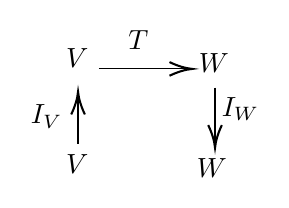
\begin{tikzpicture}[x=0.75pt,y=0.75pt,yscale=-1,xscale=1]\draw    (129,193.27) -- (129,170.27) ;\draw [shift={(129,168.27)}, rotate = 90] [color={rgb, 255:red, 0; green, 0; blue, 0 }  ][line width=0.75]    (10.93,-3.29) .. controls (6.95,-1.4) and (3.31,-0.3) .. (0,0) .. controls (3.31,0.3) and (6.95,1.4) .. (10.93,3.29)   ;\draw    (195,166.27) -- (195,193.27) ;\draw [shift={(195,195.27)}, rotate = 270] [color={rgb, 255:red, 0; green, 0; blue, 0 }  ][line width=0.75]    (10.93,-3.29) .. controls (6.95,-1.4) and (3.31,-0.3) .. (0,0) .. controls (3.31,0.3) and (6.95,1.4) .. (10.93,3.29)   ;\draw    (139,157.27) -- (182,157.27) ;\draw [shift={(184,157.27)}, rotate = 180] [color={rgb, 255:red, 0; green, 0; blue, 0 }  ][line width=0.75]    (10.93,-3.29) .. controls (6.95,-1.4) and (3.31,-0.3) .. (0,0) .. controls (3.31,0.3) and (6.95,1.4) .. (10.93,3.29)   ;\draw (122,146.4) node [anchor=north west][inner sep=0.75pt]    {$V$};\draw (122,197.4) node [anchor=north west][inner sep=0.75pt]    {$V$};\draw (186,148.4) node [anchor=north west][inner sep=0.75pt]    {$W$};\draw (185,199.4) node [anchor=north west][inner sep=0.75pt]    {$W$};\draw (105,173.4) node [anchor=north west][inner sep=0.75pt]    {$I_{V}$};\draw (197,169.67) node [anchor=north west][inner sep=0.75pt]    {$I_{W}$};\draw (152,137.67) node [anchor=north west][inner sep=0.75pt]    {$T$};\end{tikzpicture}$\pqde$\end{center} Finally, we will show the distributive properties. Note that \[\begin{aligned} [(S_1+S_2)T](v)=(S_1+S_2)(Tv)&=S_1(Tv)+S_2(Tv)\\&=(S_1T)(v)+(S_2T)(v)\\&=(S_1T+S_2T)(v).\end{aligned}\] Similarly, we can show \[\begin{aligned} [S(T_1+T_2)](v)=S[(T_1+T_2)(v)]&=S(T_1v+T_2v)\\&=S(T_1v)+S(T_2v)\\&=(ST_1)(v)+(ST_2)(v)\\&=(ST_1+ST_2)(v).\end{aligned}\]
\end{prf}
\begin{eg}
	Suppose $D\in\L(\P(\R),\P(\R))$ is the differentiation map, and $T\in\L(\P(\R),\P(\R))$ be defined by $(Tp)(x)=x^2p(x).$ Show that $DT\neq TD$.
	\begin{prf}
		Note that $(DT)p=D(Tp)=D(x^2p(x))=2xp(x)+x^2p'(x)$. Similarly, we can compute a general formula for $TD$: $(TD)p=T(Dp)=T(p')=x^2p'(x).$ Since $2xp(x)+x^2p'(x)\neq x^2p'(x)$, we know $DT\neq TD$.
	\end{prf}
\end{eg}
\begin{thm}{}
	Let $T\in\L(V,W),$ then $T(0)=0$.
\end{thm}
\begin{prf}
	Since $T(0)=T(0+0)=T(0)+T(0)$, we know $0=T(0),$ or $T(0)=0$.	
\end{prf}
\begin{cor}
	If $T(0)\neq0,$ then $T\notin\L(V,W)$.	
\end{cor}

\newpage
\subsection{Null Spaces and Ranges}
\begin{df}{Null Space/Kernel}
	For $T\in\L(V,W),$ the \textit{null space} of $T$, denoted $\Null T$, is the subset of $V$ consisting of those vectors that $T$ maps to $0$: $\Null T=\qty{v\in V\mid Tv=0}.$
\end{df}
\begin{rmk}
	Sometimes, null space of $T$ is also called the kernal of $T$, denoted as $\ker T.$	
\end{rmk}
\begin{eg}
	\begin{enumerate}
		\item Null space of zero-mapping: Let $T$ be the zero mapping from $V$ to $W$. Since $Tv=0\quad\forall v\in V,$ we know $\Null T=V.$
		\item $D\in\L(\P(\R),\P(\R))$ as $Dp=p'$: $\Null D=\qty{a\mid a\in\R}.$
		\item $T\in\L(\F^\infty,\F^\infty)$ as $T(x_1,x_2,x_3,\cdots)=(x_2,x_3,\cdots)$: $\Null T=\qty{(a,0,0,\cdots)\mid a\in\F}.$
	\end{enumerate}	
\end{eg}
\begin{thm}{}
	Suppose $T\in\L(V,W)$. Then, $\Null T$ is a subspace of $V$.
\end{thm}
\begin{prf}
	\begin{enumerate}
		\item Note that $T(0)=0,$ so $0\in\Null T.\pqde$
		\item Suppose $u,v\in\Null T.$ Then, $Tu=Tv=0$. So, $T(u+v)=Tu+Tv=0+0=0.$ Hence, $u+v\in\Null T.\pqde$
		\item Suppose $u\in\Null T$ and $\lambda\in\F$. Then, $Tu=0$. So, $T(\lambda u)=\lambda Tu=\lambda\cdot0=0$. Therefore, $\lambda u\in\Null T.$
	\end{enumerate}	
\end{prf}
\begin{df}{Injective/Injection}
	A function $T:V\to W$ is called \textit{injective} of $Tu=Tv$ implies $u=v$.	
\end{df}
\begin{rmk}
	Sometimes, the contrapositive will be much more helpful: $T$ is injective if $u\neq v$, then $Tu\neq v$.
\end{rmk}
\begin{thm}{}
	Let	$T\in\L(V,W)$. Then, $T$ is injective if and only if $\Null T=\qty{0}.$
\end{thm}
\begin{prf}
	\par ($\Rightarrow$) Suppose $T$ is an injective. We've already known that $\qty{0}\subseteq\Null T$. Then, we need to show $\Null T\subseteq\qty{0}$. Suppose $v\in\Null T$, then $Tv=0$. However, since $T$ is an injection, and $Tv=T0=0,$ then we have $v=0.$ So, $\Null T\subseteq\qty{0}$. Therefore, it's sufficient to say $\Null T=\qty{0}.\pqde$
	\par ($\Leftarrow$) Suppose $\Null T=\qty{0}$. Suppose $u,v\in V$ and $Tu=Tv.$ Then, $Tu-Tv=T(u-v)=0.$ Hence, $u-v\in\Null T$. By $\Null T=\qty{0},$ we know $u-v=0,$ so $u=v.$ Then, $T$ is an injection.
\end{prf}
\begin{df}{Range/Image}
	For $T\in\L(V,W)$, the range of $T$ is the subset of $W$ consisting of those vectors that are of the form $Tv$ for some $v\in V$: $\range T=\qty{Tv\mid v\in V}.$
\end{df}
\begin{thm}{}
	If $T\in\L(V,W)$, then $\range T$ is a subspace of $W$.	
\end{thm}
\begin{prf}
	\begin{enumerate}
		\item Since $T(0)=0,$ we know $0\in\range T.\pqde$
		\item Suppose $w_1,w_2\in\range T$. Then, $\exists v_1,v_2\in V\st Tv_1=w_1$ and $Tv_2=w_2$. Then, $w_1+w_2=Tv_1+Tv_2=T(v_1+v_2)$. Since $v_1+v_2\in V,$ we have $w_1+w_2=T(v_1+v_2)\in\range T.\pqde$
		\item Suppose $w\in\range T$ and $\lambda\in\F$. Then, $\exists v\in V\st w=Tv$. So, $\lambda w=\lambda (Tv)=T(\lambda v).$ Since $\lambda v\in V,$ $\lambda w=T(\lambda v)\in\range T.$
	\end{enumerate}	
\end{prf}
\begin{df}{Surjective/Surjection}
	A function $T:V\to W$ is called \textit{surjective} if $\range T=W$.	
\end{df}
\begin{rmk}
	A function $T:V\to W$ is called a \emph{bijection}, or is bijective, if it is both injective and surjective.	
\end{rmk}
\begin{thm}{Fundamental Theorem of Linear Maps}
	Suppose $V$ is $\FD$ and $T\in\L(V,W)$. Then, $\range T$ is $\FD$ and \[\dim V=\dim\Null T+\dim\range T.\]
\end{thm}
\begin{prf}
	Let $u_1,\cdots,u_m$ be a basis of $\Null T.$ Then, $\dim\Null T=m.$ By Theorem 3.2.3, we know $\Null T$ is a basis of $V$, so we can extend the basis to a basis of $V$: $u_1,\cdots,u_m,v_1,\cdots,v_n$. Thus, $\dim V=m+n$. \textit{WTS: $\dim\range T=n$. Further WTS: $Tv_1,\cdots,Tv_n$ is a basis of $\range T$.}\par 
	Suppose $v\in V.$ Then \[v=a_1u_1+\cdots+a_mu_m+b_1v_1+\cdots+b_nv_n.\] Since $u_1,\cdots,u_m\in\Null T,$ we know $Tu_1,\cdots,Tu_m=0.$ Therefore, \[Tv=a_1Tu_1+\cdots+a_mTu_m+b_1Tv_1+\cdots+b_nTv_n=b_1Tv_1+\cdots+b_nTv_n.\] Hence, $\span(Tv_1,\cdots,Tv_n)=\range T,$ and thus range $T$ is $\FD$. \textit{Now, WTS: $Tv_1,\cdots,Tv_n$ is $\LI$.}\par 
	Consider $c_1Tv_1+\cdots+c_nTv_n=0.$ Then, $T(c_1v_1+\cdots+c_nv_n)=0.$ Hence, $c_1v_1+\cdots+c_nv_n\in\Null T.$ Since $u_1,\cdots,u_m$ is a basis of $\Null T,$ we know \[c_1v_1+\cdots+c_nv_n=d_1u_1+\cdots+d_mu_m\quad\fs d_i\in\F.\] So, \begin{equation}\label{eq8}c_1v_1+\cdots+c_nv_n-d_1u_1-\cdots-d_mu_m=0.\end{equation} However, by assumption, we know $v_1,\cdots,v_n,u_1,\cdots,u_m$ is a basis of $V$, and thus it is $\LI.$ So, the only way to make Equation (\ref{eq8}) hold is by taking $c_1=\cdots=c_n=-d_1=\cdots=-d_m=0.$ Therefore, we've shown $Tv_1,\cdots,Tv_n$ is $\LI$, and thus is a basis of $\range T.$ Then, $\dim\range T=n.$\par 
	So, we've shown that $\dim\Null T+\dim\range T=m+n=\dim V.$
\end{prf}
\begin{thm}{}
	Suppose $V$ and $W$ are $\FD$ vector spaces $\st$ $\dim V>\dim W.$ Then, no linear map from $V$ to $W$ is injective.
\end{thm}
\begin{prf}
	Let $T\in\L(V,W)$. By the Fundamental Theorem of Linear Maps, we have $\dim V=\dim\Null T+\dim\range T$. Then, we know \[\begin{aligned}\dim\Null T&=\dim V-\dim\range T\\&\geq\dim V-\dim W>0&[\dim\range T\leq\dim W]\end{aligned}\] This implies that $\Null T\neq\qty{0}.$ So, $T$ is not injective by Theorem 3.2.5.
\end{prf}
\begin{thm}{}
	Suppose $V$ and $W$ are $\FD$ vector space $\st \dim V<\dim W$. Then, no linear map from $V$ to $W$ is surjective.	
\end{thm}
\begin{prf}
	We know \[\begin{aligned}\dim\range T&=\dim V-\dim\Null T\\&\leq\dim V<\dim W\end{aligned}\]	Then, $T$ cannot be surjective by definition. 
\end{prf}
\begin{eg} Solving Linear Systems Using Linear Maps I\par 
	For a homogenous system of linear equations, \[\begin{cases}A_{1,1}x_1+\cdots+A_{1,n}x_n=0\\\qquad\qquad\vdots\\A_{m,1}x_1+\cdots+A_{m,n}x_n=0\end{cases},\] where $A_{j,k}\in\F$ and $(x_1,\cdots,x_n)\in\F^n,$ we can defined a linear map $T:\F^n\to\F^m$ as \[T(x_1,\cdots,x_n)=\qty(\sum_{k=1}^nA_{1,k}x_k,\cdots,\sum_{k=1}^nA_{m,k}x_k).\] 	Apparently, $(x_1,\cdots,x_n)=0$ is a solution to the system, but the question is ``If there are any non-zero solutions for this linear system?''
\end{eg}
\begin{thm}{}
	A homogeneous system of linear equations with more variables than equations has non-zero solutions.
\end{thm}
\begin{prf}
	Suppose $T\in\L(V,W)$. Then, $\dim V=n$ and $\dim W=m$. Suppose $n>m.$ So, $\dim V>\dim W.$ By the Theorem 3.2.5, we know $T$ is not injective.
\end{prf}
\begin{eg} Solving Linear Systems Using Linear Maps II\par 
	For an inhomogeneous system of linear equations \[\begin{cases}\dsst\sum_{k=1}^nA_{1,k}x_k=c_1\\\qquad\vdots\\\dsst\sum_{k=1}^nA_{m,k}x_k=c_m\end{cases},\] where $A_{j,k}\in\F$ and $(c_1,\cdots,c_m)\in\F^m$ and $(x_1,\cdots,x_n)\in\F^n,$ we can define $T:\F^n\to\F^m$ by \[T(x_1,\cdots,x_m)=\qty(\dsst\sum_{k=1}^nA_{1,k}x_k,\cdots,\dsst\sum_{k=1}^nA_{m,k}x_k=c_1).\] However, in this case, $(x_1,\cdots,x_n)=0$ may not be a solution to the system.
\end{eg}
\begin{thm}{}
	An inhomogeneous system of linear equations with more equations than variables has no solution for some choice of the constant terms.
\end{thm}
\begin{prf}
	Suppose	$T\in\L(V,W)$. So, $\dim V=n$ and $\dim W=m.$ Suppose $n<m.$ Then, $\dim V<\dim W.$ By Theorem 3.2.11, we know $T$ is not surjective.
\end{prf}

\newpage
\subsection{Matrices}
\begin{df}{Matrix}
	Let $m,n\in\Zp$. An \textit{$m$-by-$n$ matrix $A$} is a rectangular array of elements of $\F$ with $m$ rows and $n$ columns: \[A=\mqty(A_{1,1}&\cdots&A_{1,n}\\\vdots&&\vdots\\A_{m,1}&\cdots&A_{m,n}).\] The notation $A_{j,k}$ denotes the entry in row $j$, column $k$ of $A$.
\end{df}
\begin{df}{Matrix of a Linear Map}
	Suppose $T\in\L(V,W)$	 and $v_1,\cdots,v_n$ is a basis of $V$ and $w_1,\cdots,w_m$ is a basis of $W$. The \textit{matrix of $T$} with respect to these bases is the $m\times n$ matrix $\M(T)$ whose $A_{j,k}$ are defined by \[Tv_k=A_{1,k}w_1+\cdots+A_{m,k}w_m.\] If the bases are not clear from the context, then the notation $\M(T,(v_1,\cdots,v_n),(w_1,\cdots,w_m))$ is used.
\end{df}
\begin{eg}
	Suppose $T\in\L(\F^2,\F^3)$ is defined by $T(x,y)=(x+3y,2x+5y,7x+9y).$ Find the matrix of $T$ with respect to the standard bases of $\F^2$ and $\F^3.$
	\begin{sol}
		Note that $T(1,0)=(1,2,7)$ and $T(0,1)=(3,5,9)$. Then, \[\M(T)=\mqty(1&3\\2&5\\7&9).\]
	\end{sol}
\end{eg}
\begin{eg}
	Suppose $D\in\L(\P_3(\R),\P_2(\R))$ is the differentiation map defined by $Dp=p'$. Find the matrix of $D$ with respect to the standard bases of $\P_3(\R)$ and $\P_2(\R)$.
	\begin{sol}
		Standard bases of $\P_3(\R):$ $1,x,x^2,x^3.$ Standard bases of $\P_2(\R):$ $1,x,x^2.$ Since $(x^n)'=nx^{n-1},$ so we have \[\begin{aligned}D(1)&=0=0\cdot1+0\cdot x+0\cdot x^2\\D(x)&=1=1\cdot1+0\cdot x+0\cdot x^2\\D(x^2)&=2x=0\cdot1+2\cdot x+0\cdot x^2\\D(x^3)&=3x^2=0\cdot1+0\cdot x+3\cdot x^2\end{aligned}\] So, we have \[\M(D)=\mqty(0&1&0&0\\0&0&2&0\\0&0&0&3).\]
	\end{sol}
\end{eg}
\begin{df}{Matrix Addition}
	The \textit{sum of two matrices of the same size} is the matrix obtained by adding corresponding entries in the matrices: \[\mqty(A_{1,1}&\cdots&A_{1,n}\\\vdots&&\vdots\\A_{m,1}&\cdots&A_{m,n})+\mqty(C_{1,1}&\cdots&C_{1,n}\\\vdots&&\vdots\\C_{m,1}&\cdots&C_{m,n})=\mqty(A_{1,1}+C_{1,1}&\cdots&A_{1,n}+C_{1,n}\\\vdots&&\vdots\\A_{m,1}+C_{m,1}&\cdots&A_{m,n}+C_{m,n}).\]	
\end{df}
\begin{thm}{}
	Suppose $S,T\in\L(V,W).$ Then, $\M(S+T)=\M(S)+\M(T).$
\end{thm}
\begin{prf}
	Let $v_1,\cdots,v_n$ be a basis of V and $w_1,\cdots,w_n$ be a basis of $W$. Suppose $\M(S)=A$ and $\M(T)=C.$ Then, if $1\leq k\leq n,$ we have\[\begin{aligned}(S+T)v_k&=Sv_k+Tv_k\\&=(A_{1,k}w_1+\cdots+A_{m,k}w_m)+(C_{1,k}w_1+\cdots+C_{m,k}w_m)\\&=(A_{1,k}+C_{1,k})w_1+\cdots+(A_{m,k}+C_{m,k})w_m.\end{aligned}\]	Hence, we have $\M(S+T)=\M(S)+\M(T).$
\end{prf}
\begin{df}{Scalar Multiplication of a Matrix}
	The \textit{product of a scalar and a matrix} is the matrix obtained by multiplying each entry in the matrix by the scalar: \[\lambda\mqty(A_{1,1}&\cdots&A_{1,n}\\\vdots&&\vdots\\A_{m,1}&\cdots&A_{m,n})=\mqty(\lambda A_{1,1}&\cdots&\lambda A_{1,n}\\\vdots&&\vdots\\\lambda A_{m,1}&\cdots&\lambda A_{m,n}).\] In other words, $(\lambda A)_{j,k}=\lambda A_{j,k}.$
\end{df}
\begin{thm}{}
	Suppose	$\lambda\in\F$ and $T\in\L(V,W)$. Then, $\M(\lambda T)=\lambda\M(T).$
\end{thm}
\begin{prf}
	Let $v_1,\cdots,v_n$ be a basis of V and $\M(T)=A.$ When $1\leq k\leq v$, note that \[\begin{aligned}(\lambda T)v_k&=\lambda(Tv_k)\\&=\lambda(A_{1,k}w_1+\cdots+A_{m,k}w_m)\\&=(\lambda A_{1,k})w_1+\cdots+(\lambda A_{m,k})w_m.\end{aligned}\] So, $\M(\lambda T)=\lambda\M(T).$
\end{prf}
\begin{nota}
	$\F^{m,n}\coloneqq$ the set of all $m\times n$ matrices with entries in $\F$.	
\end{nota}
\begin{thm}{}
	Suppose $m,n\in\Zp.$ With addition and scalar multiplication defined above, $\F^{m,n}$ is a vector space and $\dim\F^{m,n}=mn.$
\end{thm}
\begin{prf}
	It is trivial to prove $\F^{m,n}$ is a vector space.$\pqde$\par Define $A_{j,k}$ as the matrix with $1$ on its $j^\text{th}$ row, $k^\text{th}$ column and $0$ elsewhere. Then, we can see that $A_{j,k}$ for $j=1,\cdots,m$ and $k=1,\cdots,n$ is a basis for $\F^{m,n}.$ So, $\dim\F^{m,n}=m\cdot n.$	
\end{prf}
\begin{df}{Matrix Multiplication}
	Suppose $A$ is an $m\times n$ matrix and $C$ is an $n\times p$ matrix. Then, $AC$ is defined to be the $m\times p$ matrix whose entry in row $j$. column $k$ is given by \[(AC)_{j,k}=\sum_{r=1}^nA_{j,r}C_{r,k}.\]	
\end{df}
\begin{rmk}
	Matrix multiplication is not commutative. i.e., $AC\neq CA$. However, it is distributive and associative.	
\end{rmk}
\begin{thm}{}
	If $T\in\L(U,V)$ and $S\in\L(V,W),$ then $\M(ST)=\M(S)\M(T)$.
\end{thm}
\begin{nota}
	Suppose $A$ is an $m\times n$ matrix.
	\begin{enumerate}
		\item If $1\leq j\leq m,$ then $A_{j,\cdot}$ denotes the $1\times n$ matrix consisting of row $j$ of $A$.
		\item If $1\leq k\leq n$, then $A_{\cdot,k}$ denotes the $m\times1$ matrix consisting of column $k$ of $A$.
	\end{enumerate}	
	In other words, \[A=\mqty(A_{1,1}&\cdots&A_{1,n}\\\vdots&&\vdots\\A_{m,1}&\cdots&A_{m,n});\qquad A_{j,\cdot}=\mqty(A_{j,1}&\cdots&A_{j,n})\in\F^{1,n};\qquad A_{\cdot,k}=\mqty(A_{1,k}\\\vdots\\A_{m,k})\in\F^{m,1}.\]
\end{nota}
\begin{thm}{Practical Interpretations of Matrix Multiplication}
	\begin{enumerate}
		\item Suppose $A$ is an $m\times n$ matrix and $C$ is an $n\times p$ matrix. Then, $(AC)_{j,k}=A_{j,\cdot}C_{\cdot,k}$ for $1\leq j\leq m$ and $1\leq k\leq p.$
		\item Suppose $A$ is an $m\times n$ matrix and $C$ is an $n\times p$ matrix. Then, $(AC)_{\cdot,k}=AC_{\cdot,k}$ for $1\leq k\leq p.$
		\item Suppose $A$ is an $m\times n$ matrix and $C=\mqty(c_1\\\vdots\\c_n)$ is an $n\times1$ matrix. Then, \[AC=c_1A_{\cdot,1}+\cdots+c_nA_{\cdot,n}.\] In other words, $AC$ is a linear combination of the columns of $A$, with the scalars that multiply the columns coming from $C$.
	\end{enumerate}	
\end{thm}
\begin{eg}
	\[\mqty(1&2\\3&4\\5&6)\mqty(5\\1)=5\mqty(1\\3\\5)+1\mqty(2\\4\\6)=\mqty(7\\19\\31).\]	
\end{eg}

\newpage
\subsection{Invertibility and Isomorphic Vector Spaces}
\begin{df}{Invertible}
	A linear map $T\in\L(V,W)$ is called \textit{invertible} if $\exists$ a linear map $S\in\L(W,V)\st ST$ equals the identity map on $I$ and $TS$ equals the identity map on $W$.	
\end{df}
\begin{df}{Inverse}
	A linear map $S\in\L(W,V)$ satisfying $ST=I$ and $TS=I$ is called an \textit{inverse} of $T$.	
\end{df}
\begin{thm}{}
	An invertible linear map has a unique inverse.	
\end{thm}
\begin{prf}
	Suppose $T\in\L(V,W)$ is invertible. Let $S_1$ and $S_2$ be inverses of $T$.Then, \[S_1=S_1I=S_1(TS_2)=(S_1T)S_2=IS_2=S_2.\] Thus, $S_1=S_2,$ and so inverse is unique.
\end{prf}
\begin{nota}
	If $T$ is invertible, then its inverse is denoted by $\T.$	
\end{nota}
\begin{thm}{}
	A linear map is invertible if and only if it is injective and surjective.
\end{thm}
\begin{prf}
	\par ($\Rightarrow$) Let $T\in\L(V,W)$ be invertible. Then, $T\T=I_W$ and $\T T=T_V$. Let $Tv=0$. Note that $(\T T)v=0,$ so $Iv=0$ and thus $v=0$. Therefore, $\Null T=\qty{0}$, and so $T$ is an injection. 
	\par To show $T$ is surjective, suppose $w\in W.$ Note that since $\T\in\L(W,V),$ $\T w\in V.$ So, \[T(\T w)=(T\T)w=T_Ww=w\in W.\] Therefore, $\T w$ is the $v\in V$ we intend to find. Hence, $T$ is also a surjection. $\pqde$
	\par ($\Leftarrow$) Let $T$ be surjective and injective. For $w\in W,$ define $Sw\in V\st T(Sw)=w.$ So, we know $Sw$ is unique. Since $(T\of S)w=w,$ we know $(T\of S)=I_W.$ Consider $(S\of T)v=S(Tv),$ we have $T(S(Tv))=Tv,$ by definition of $S$. Since $T$ is injective, we know $S(Tv)=V.$ So, $(S\of T)v=v,$ and thus $ST=T_V.$ Therefore $T$ is invertible.
	\par Now, we want to show $S$ is a linear map. Let $w_1,w_2\in W,$ then \[T(S(w_1+w_2))=(TS)(w_1+w_2)=I_W(w_1+w_2)=w_1+w_2.\] By definition, $w_1+w_2=T(Sw_1)+T(Sw_3)=T(Sw_1+Sw_2).$ So, $T(S(w_1+w_2))=T(Sw_1+Sw_2).$ By $T$ is an injection, we have $S(w_1+w_2)=Sw_1+Sw_2.$ So, $S$ is additive. Further consider \[T(S(\lambda w))=\lambda w=\lambda(T(Sw))=T(\lambda Sw)\] for some $w\in W.$ Again, since $T$ is injective, $S(\lambda w)=\lambda Sw.$ So, $S$ has homogeneity. Then, $S$ is a linear map.
\end{prf}
\begin{df}{Isomorphism}
	An \textit{isomorphism} is an invertible linear map. 	
\end{df}
\begin{df}{Isomorphic}
	Two vector spaces are called \textit{isomorphic} if there is an isomorphism from one vector space onto the other one.	
\end{df}
\begin{nota}
	If two vector spaces $V$ and $W$ are isomorphic, we denote them as $V\cong W.$	
\end{nota}
\begin{thm}{}
	Suppose $V$ and $W$ are $\FD$ vector spaces, then $V\cong W$ if and only if $\dim V=\dim W.$	
\end{thm}
\begin{prf}
	\par ($\Rightarrow$) Suppose $V\cong W.$ By Fundamental Theorem of Linear Maps, we know \[\dim V=\dim\Null T+\dim\range T.\] Since $V\cong W,$ $T$ is invertible and thus is injective and surjective. So, $\dim\Null T=0$ and $\dim\range T=\dim W.$ Therefore, $\dim V=0+\dim W=\dim W.\pqde$
	\par ($\Leftarrow$)	Suppose $\dim V=\dim W.$ Suppose $v_1,\cdots,v_n$ and $w_1,\cdots,w_n$ are bases of $V$ and $W$, respectively. Then, $\dim V=\dim W=n.$ Here, we want to define a bijection between $V$ and $W$. Let $T$ be defined as $Tv_i=wi\quad(i=1,\cdots,n).$\par 
	Let $Tv=0$. Then, $T(a_1v_1+\cdots+a_nv_n)=0$. So, by definition, $a_1w_1+\cdots+a_nw_n=0.$ Since $w_1,\cdots,w_n$ is a basis, we have $a_1=\cdots=a_n=0$. So, $\Null T=\qty{0},$ and thus $T$ is an injection.\par 
	Let $w\in W$ be any vector. Then, we know $w=c_1w_1+\cdots+c_nw_n$. Note that, by definition of $T$, we have $T(c_1v_1+\cdots+c_nv_n)=c_1w_1+\cdots+c_nw_n$. Hence, $\forall w\in W,\exists v=c_1v_1+\cdots+c_nv_n\in V\st Tv=w.$ Therefore, $T$ is a surjection.\par 
	Finally, it is trivial to show that $T$ is indeed a linear map, and so the proof is complete.
\end{prf}
\begin{thm}{}
	Suppose $v_1,\cdots,v_n$ is a basis of $V$ and $w_1,\cdots,w_m$ is a basis of $W$. then, $\M$ is an isomorphism between $\L(V,W)$ and $\F^{m,n}.$	
\end{thm}
\begin{prf}
	We already know $\M$ is linear, so we just need to show $\M$ is a bijection. \par 
	To prove $\M$ is injective, consider $\M(T)=0$ for some $T\in\L(V,W)$. So, we get $Tv_k=0$. Since $v_1,\cdots,v_n$ is a basis of $V$, we know $Tv=0\quad\forall v\in V$. Then, $T$ is the zero-mapping, or $T=0$. Therefore, $\Null\M=\qty{0}$.\par 
	To show $\M$ is surjective, suppose $A\in\F^{m,n}$. Let $T$ be a linear map from $V$ to $W\st$ \[Tv_k=\dsst\sum_{j=1}^mA_{j,k}w_j,\quad k=1,\cdots,n.\] Obviously, $\M(T)=A$, and thus $\range\M=\F^{m,n}$. So, $\M$ is also a surjection.
\end{prf}
\begin{thm}{}
	Suppose $V$ and $W$ are $\FD$. Then, $\L(V,W)$ is $\FD$ and $\dim\L(V,W)=(\dim V)(\dim W).$	
\end{thm}
\begin{prf}
	By Theorem 3.4.10 and Theorem 3.4.9, we know $\dim\L(V,W)=\dim\F^{m,n}.$ Further by Theorem 3.3.10, we know $\dim\F^{m,n}=(m)(n).$ As $\dim V=n$ and $\dim W=m$, so we have \[\dim\L(V,W)=(\dim V)(\dim W).\]	
\end{prf}
\begin{df}{Matrix of a Vector, $\M(v)$}
	Suppose $v\in V$ and $v_1,\cdots,v_n$ is a basis of $V$. The \textit{matrix of $v$} with respect to this basis is the $n\times1$ matrix \[\M(v)=\mqty(c_1\\\vdots\\c_n),\] where $c_1,\cdots,c_n$ are scalars $\st v=c_1v_1+\cdots+c_nv_n$.
\end{df}
\begin{thm}{$\M(T)_{\cdot,k}=\M(v_k)$}
	Suppose $T\in\L(V,W)$ and $v_1,\cdots,v_n$ is a basis of $V$ and $w_1,\cdots,w_m$ is a basis of $W$. Let $1\leq k\leq n$. Then, the $k^\text{th}$ column of $\M(T)$, which is denoted by $\M(T)_{\cdot,k}$, equals $\M(v_k)$.
\end{thm}
\begin{prf}
	This theorem is an immediate result by definitions of matrix of a linear mapping and a vector. 	
\end{prf}
\begin{thm}{}
	Suppose $T\in\L(V,W)$ and $v\in V$. Suppose $v_1,\cdots,v_n$ is a basis of $V$ and $w_1,\cdots,w_m$ is a basis of $W$. Then, $\M(Tv)=\M(T)\M(v).$	
\end{thm}
\begin{prf}
	Note that $v=c_1v_1+\cdots+c_nv_n,$ so we have $Tv=c_1Tv_1+\cdots+c_nTv_n$. So, by Theorem 3.4.13, we know \[\begin{aligned}\M(Tv)&=c_1\M(Tv_1)+\cdots+c_n\M(Tv_n)\\&=c_1\M(T)_{\cdot,1}+\cdots+c_n\M(T)_{\cdot,n}\\&=\M(T)\M(v).\end{aligned}\] The final equality holds due to our interpretation of matrix multiplication as column linear combinations (Theorem 3.3.14(3))
\end{prf}
\begin{rmk}
	$\M:\F^n\to\F^{n,1}$ is an isomorphism: \[v=c_1v_1+\cdots+c_nv_n\longmapsto\mqty(c_1\\\vdots\\c_n).\]	
\end{rmk}
\begin{prf}
	Suppose $\M(v)=0:\ \M(c_1v_1+\cdots+c_nv_n)=0$. So, we have $c_1w_1+\cdots+c_nw_n=0$. Since $w_1,\cdots,w_n$ is a basis, $c_1=\cdots=c_n=0$. So, $v=0$. Therefore, $\Null\M=\qty{0}$, and so $\M$ is injective.$\pqde$\par 
	Now, prove $\M$ is surjective. Note that $\forall\mqty(c_1\\\vdots\\c_n)$, we have $\M(c_1v_1+\cdots+c_nv_n)=\mqty(c_1\\\vdots\\c_n)$. So, $\M$ is a surjection. $\pqde$\par 
	Finally, its' trivial to prove $\M$ is a linear map. $\pqde$\par 
	Since $\M$ is both surjective and injective, $\M$ is an isomorphism. 	
\end{prf}
\begin{df}{Operator}
	A linear map from a vector space to itself is called an \textit{operator}.
\end{df}
\begin{nota}
	The notation $\L(V)$ denotes the set of all operators on $V$. So, $\L(v)=\L(V,V)$.	
\end{nota}
\begin{thm}{}
	Suppose $V$ is $\FD$ and $T\in\L(V)$. Then, the following are equivalent: (a) $T$ is invertible; (b) $T$ is injective; and (c) $T$ is surjective. 
\end{thm}
\begin{prf}
	\begin{enumerate}
		\item Clearly (a) implies (b). $\pqde$
		\item Suppose (b): $T$ is injective. So, $\Null T=\qty{0}$. Then, by Fundamental Theorem of Linear Maps, we know \[\dim V=\dim\Null T+\dim\range T=0+\dim\range T.\] Since $\dim\range T=\dim V,$ we know $T$ is surjective. $\pqde$
		\item Suppose (c): $T$ is surjective. So, $\range T=V$. Then, by Fundamental Theorem of Linear maps, we have \[\dim\Null T=\dim V-\dim\range T=0.\] So, $\Null T=\qty{0},$ and thus $T$ is injective. Since $T$ is surjective and injective, $T$ is invertible. 
	\end{enumerate}	
\end{prf}
\begin{eg}
	Show that for each polynomial $q\in\P(\R),$ there exists a polynomial $p\in\P(\F)$ such that $((x^2+5x+7)p)''=q$.
\end{eg}
\begin{prf}
	We know that every non-zero polynomial must have a degree of $m$. So, we can think of this problem under $\P_m(\R)$. Note that \[((x^2+5x+7)p)''=2p+(4x+10)p'+(x^2+5x+7)p''=q.\] Therefore, the degree of $p$ and $q$ should be the same. Define $T:\P_m(\R)\to\P_m(\R)$ as \[Tp=((x^2+5x+7)p)''.\] Then, $T$ is an operator on $\P_m(\R)$. Consider $Tp=0$. We have $ax+b=(x^2+5x+7)p$. Note that only when $p=0$, the equation above holds. So, it must be that $p=0$ when $Tp=0$. That is, $\Null T=\qty{0}$, and so $T$ is injective. By Theorem 3.4.18, we know $T$ is also surjective, and so our proof is complete.
\end{prf}

\newpage
\subsection{Duality}
\begin{df}{Linear Functional}
	A \textit{linear functional} on $V$ is a linear map from $V$ to $\F$. That is, a linear functional is an element of $\L(V,\F)$.	
\end{df}
\begin{eg}
	\begin{enumerate}
		\item Fix $(c_1,\cdots,c_n)\in\F^n$. Define $\phi:\F^n\to\F$ by $\phi(x_1,\cdots,x_n)=c_1x_1+\cdots+c_nx_n$. Then, $\phi$ is a linear functional on $\F^n$.
		\item Define $\phi:\P(\R)\to\R$ as $\phi(p)=3p''(5)+7p(4)$.
		\item Define $\phi:\P(\R)\to\R$ as $\phi(p)=\dsst\int_0^1p(x) \d x$.
	\end{enumerate}	
\end{eg}
\begin{df}{Dual Space/$V'$/$V^*$}
	The \textit{dual space} of $V$, denoted as $V'$, is the vector space of all linear functionals on $V$. In other words, $V'=\L(V,\F)$.
\end{df}
\begin{thm}{}
	Suppose $V$ is $\FD$. Then, $V'$ is also $\FD$ and $\dim V'=\dim V$.	
\end{thm}
\begin{prf}
	Note that for a general linear map, $\L(V,W)\cong\F^{m,n}$. So, $\L(V,\F)=V'\cong\F^{1,n}$. Hence, \[\dim V'=\dim\F^{1,n}=1\cdot n=n=\dim V.\]	
\end{prf}
\begin{df}{Dual Basis}
	If $v_1,\cdots,v_n$ is a basis of $V$, then the \textit{dual basis} of $v_1,\cdots,v_n$ is the list $\phi_1,\cdots,\phi_n$ of elements of $V'$, where each $\phi_j$ is the linear functional on $V\st$ \[\phi_j(v_k)=\begin{cases}1\quad\text{if }k=j\\0\quad\text{if }k\neq j\end{cases}.\]
\end{df}
\begin{eg}
	Find the dual basis of $e_1,\cdots,e_n\in\F^n$	
\end{eg}
\begin{sol}
	\begin{center}
	\begin{tabular}{cccc}
		$\phi_1(e_1)=1$&$\phi_2(e_1)=0$&$\cdots$&$\phi_n(e_1)=0$\\
		$\phi_1(e_2)=0$&$\phi_2(e_2)=1$&$\cdots$&$\phi_n(e_2)=0$\\
		$\vdots$&$\vdots$&$\ddots$&$\vdots$\\
		$\phi_1(e_n)=1$&$\phi_2(e_n)=0$&$\cdots$&$\phi_n(e_n)=1$
	\end{tabular}
	\end{center}
	Define $\phi_j$ as \[\phi_j(x)=\phi_j(x_1,\cdots,x_n)=x_1\phi_j(e_1)+\cdots+x_j\phi_j(e_j)+\cdots+x_n\phi_j(e_n)=x_j.\]
\end{sol}
\begin{thm}{}
	Suppose $V$ is $\FD$. Then, the dual basis of a basis of $V$ is a basis of $V'$.	
\end{thm}
\begin{prf}
	Suppose $v_1,\cdots,v_n$ is a basis of $V$ and $\phi_1,\cdots,\phi_n$ denotes the dual basis. Since we've shown $\dim V=\dim V'$ in Theorem 3.5.4, we only need to show $\phi_1,\cdots,\phi_n$ is $\LI.$	Select $c_1\phi_1+\cdots+c_n\phi_n=0$. Then, \[(c_1\phi_1+\cdots+c_n\phi_n)(v)=0\quad\forall\ v\in V.\] Suppose $v=v_1+\cdots+v_n$, then \[(c_1\phi_1+\cdots+c_n\phi_n)(v_j)=c_j\quad\text{for }j=1,\cdots,n.\] So, $(c_1\phi_1+\cdots+c_n\phi_n)(v)=c_1+\cdots+c_n=0$. So, it must be that $c_1=\cdots=c_n=0$. Therefore, $\phi_1,\cdots,\phi_n$ is $\LI$ and our proof is complete. 
\end{prf}
\begin{df}{Dual Map}
	If $T\in\L(V,W)$, then the \textit{dual map} of $T$ is the linear map $T'\in\L(W',V')$ defined by $T'(\phi)=\phi\of T$ for $\phi\in W'$.	
\end{df}
\begin{rmk}	The following diagram represents dual map (but not an exact representation).
	\begin{center}
		\tikzset{every picture/.style={line width=0.75pt}}
		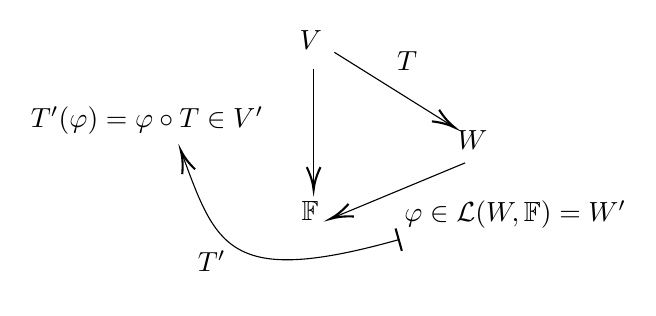
\begin{tikzpicture}[x=0.75pt,y=0.75pt,yscale=-1,xscale=1]
		\draw    (201,75) -- (257.31,110.21) ;
		\draw [shift={(259,111.27)}, rotate = 212.02] [color={rgb, 255:red, 0; green, 0; blue, 0 }  ][line width=0.75]    (10.93,-3.29) .. controls (6.95,-1.4) and (3.31,-0.3) .. (0,0) .. controls (3.31,0.3) and (6.95,1.4) .. (10.93,3.29)   ;
		\draw    (191,83.27) -- (191,139.27) ;
		\draw [shift={(191,141.27)}, rotate = 270] [color={rgb, 255:red, 0; green, 0; blue, 0 }  ][line width=0.75]    (10.93,-3.29) .. controls (6.95,-1.4) and (3.31,-0.3) .. (0,0) .. controls (3.31,0.3) and (6.95,1.4) .. (10.93,3.29)   ;
		\draw    (264,128.27) -- (200.85,154.51) ;
		\draw [shift={(199,155.27)}, rotate = 337.44] [color={rgb, 255:red, 0; green, 0; blue, 0 }  ][line width=0.75]    (10.93,-3.29) .. controls (6.95,-1.4) and (3.31,-0.3) .. (0,0) .. controls (3.31,0.3) and (6.95,1.4) .. (10.93,3.29)   ;
		\draw    (232,165.27) .. controls (149.84,188.31) and (144.11,168.67) .. (127.51,123.64) ;
		\draw [shift={(127,122.27)}, rotate = 69.72] [color={rgb, 255:red, 0; green, 0; blue, 0 }  ][line width=0.75]    (10.93,-3.29) .. controls (6.95,-1.4) and (3.31,-0.3) .. (0,0) .. controls (3.31,0.3) and (6.95,1.4) .. (10.93,3.29)   ;
		\draw [shift={(232,165.27)}, rotate = 344.34] [color={rgb, 255:red, 0; green, 0; blue, 0 }  ][line width=0.75]    (0,5.59) -- (0,-5.59)   ;
		\draw (183,63.4) node [anchor=north west][inner sep=0.75pt]    {$V$};
		\draw (259,111.4) node [anchor=north west][inner sep=0.75pt]    {$W$};
		\draw (184,145.4) node [anchor=north west][inner sep=0.75pt]    {$\mathbb{F}$};
		\draw (230,73.4) node [anchor=north west][inner sep=0.75pt]    {$T$};
		\draw (233.5,145.17) node [anchor=north west][inner sep=0.75pt]    {$\varphi \in \mathcal{L}( W,\mathbb{F}) =W'$};
		\draw (53.5,100.17) node [anchor=north west][inner sep=0.75pt]    {$T'( \varphi ) =\varphi \circ T\in V'$};
		\draw (134,169.4) node [anchor=north west][inner sep=0.75pt]    {$T'$};
		\end{tikzpicture}
	\end{center}
	Also, dual map is a linear map, so it is additive and homogeneous.
	\begin{enumerate}
		\item $T'(\phi+\psi)=(\phi+\psi)\of T=\phi\of T+\psi\of T=T'(\phi)+T'(\psi)$.
		\item $T'(\lambda\phi)=(\lambda\phi)\of T=\lambda(\phi\of T)=\lambda T'(\phi)$.
	\end{enumerate}	
\end{rmk}
\begin{eg}
	Suppose $D:\P(\R)\to\P(\R)$ as $Dp=p'$.
	\begin{enumerate}
		\item Define a linear functional $\phi:\P(\R)\to\R$ as $\phi(p)=p(3)$. Find $D'(\phi)$. \begin{sol}\[(D'(\phi))(p)=(\phi\of D)(p)=\phi(Dp)=\phi(p')=p'(3).\]\end{sol}
		\item Define $\phi:\P(\R)\to\R$, a linear functional, as $\phi(p)=\dsst\int_0^1p(x)\ \d x$. Find $D'(\phi)$.\begin{sol}\[(D'(\phi))(p)=(\phi\of D)(p)=\phi(Dp)=\phi(p')=\int_0^1p'(x)\ \d x=p(1)-p(0).\]\end{sol}
	\end{enumerate}	
\end{eg}
\begin{thm}{Algebraic Properties of Dual Maps}
	\begin{enumerate}
		\item $(S+T)'=S'+T'\quad\forall\ S,T\in\L(V,W)$
		\item $(\lambda T)'=\lambda T'\quad\forall\ T\in\L(V,W)$
		\item $(ST)'=T'S'\quad\forall\ T\in\L(U,V)$ and $S\in\L(V,W)$
	\end{enumerate}
\end{thm}
\begin{prf}
	\begin{enumerate}
		\item $(S+T)'\in\L(W',V')$. Let $\phi\in W'$. Then, \[(S+T)'(\phi)=\phi\of(S+T)=\phi\of S+\phi\of T=S'(\phi)+T'(\phi)=(S'+T')(\phi).\pqde\]
		\item $(\lambda T)'\in\L(W',V')$. Let $\phi\in W'$. Then, \[(\lambda T)'(\phi)=\phi\of(\lambda T)=\lambda(\phi\of T)=\lambda T'(\phi)=(\lambda T')(\phi).\pqde\]
		\item $(ST)'\in\L(W',U')$. Let $\phi\in W'$. Then, \[(ST)'(\phi)=\phi\of(ST)=\phi\of(S\of T)=(\phi\of S)\of T=(S'(\phi))\of T=T'(S'(\phi))=(T'S')(\phi).\]
	\end{enumerate}	
\end{prf}
\begin{df}{Transpose/$A^t$}
	The transpose of a matrix $A$, denoted $A^t$, is the matrix obtained from $A$ by interchanging the rows and columns. i.e., $(A^t)_{k,j}=A_{j,k}.$
\end{df}
\begin{rmk}
	Transpose is additive and homogeneous. That is, $(A+C)^t=A^t+C^t$ and $(\lambda A)^t=\lambda A^t$.	
\end{rmk}
\begin{thm}{}
	If $A$ is an $m\times n$ matrix and $C$ is an $n\times p$ matrix, then $(AC)^t=C^tA^t$.
\end{thm}
\begin{prf}
	Note that \[(AC)^t_{k,j}=(AC)_{j,k}=\sum_{r=1}^nA_{j,r}C_{r,k}=\sum_{r=1}^n(C^t)_{k,r}(A^t)_{r,j}=(C^tA^t)_{k,j}\]	
\end{prf}
\begin{thm}{}
	Suppose $T\in\L(V,W)$. Then, $\M(T')=(\M(T))^t$.	
\end{thm}
\begin{prf}
	Suppose $v_1,\cdots,v_n$ is a basis of $V$, $w_1,\cdots,w_m$ is a basis of $W$, $\phi_1,\cdots,\phi_n$ is a basis of $V'$, and $\psi_1,\cdots,\psi_m$ is a basis of $W'$. Let $A=\M(T)$ and $C=\M(T')$. Since $T'(\psi_j)=C_{1,j}\phi_1+\cdots+C_{n,j}\phi_n$ and $T'(\psi_j)=\psi_j\of T$, we have $\psi_j\of T=C_{1,j}\phi_1+\cdots+C_{n,j}\phi_n$. Consider \[\begin{aligned}(\psi_j\of T)(v_k)=(C_{1,j}\phi_1+\cdots+C_{n,j}\phi_n)(v_k)=C_{k,j}\phi_k(v_k)=C_{k,j}.\end{aligned}\]	Also, we have \[(\psi_j\of T)(v_k)=\psi_j(Tv_k)=\psi_j(A_{1,k}w_1+\cdots+A_{m,k}w_m)=\psi_j(A_{j,k}w_j)=A_{j,k}(\phi_j(w_j))=A_{j,k}.\] Therefore, we have $A_{j,k}=C_{k,j}$, and thus $A=C^t$. So, $\M(T)=(\M(T'))^t$.
\end{prf}
\begin{df}{Annihilator/$U^0$}
	For $U\subseteq V,$ the \textit{annihilator} of $U$, denoted as $\Ua$, is defined by \[\Ua=\qty{\phi\in V'\mid \phi(u)=0\quad\forall u\in U}.\]
\end{df}
\begin{thm}{}
	Suppose $U\subseteq V$. Then $\Ua$ is a subspace of $V'$.	
\end{thm}
\begin{prf}
	\begin{enumerate}
		\item $0\in\Ua$: Since $0(u)=0\quad\forall u\in U,$ then $0\in\Ua.\pqde$
		\item Let $\phi,\psi\in\Ua$. Then, \[(\phi+\psi)(u)=\phi(u)+\psi(u)=0.\] So, $\phi+\psi\in\Ua.\pqde$
		\item Let $\lambda\in\F$ and $\phi\in\Ua$. Then \[(\lambda\phi)(u)=\lambda\phi(u)=\lambda\cdot0=0.\] So, $\lambda\phi\in\Ua.$
	\end{enumerate}	
\end{prf}
\begin{lem}{}
	Suppose $V$ is $\FD$ vector space. If $U$ is a subspace of $V$ and $S\in\L(U,W)$, then there exists $T\in\L(V,W)\st Tu=Su\quad\forall u\in U$.	
\end{lem}
\begin{prf}
	Suppose $u_1,\cdots,u_m$ is a basis of $U$. Then, we can extend it to a basis of $V$ as $u_1,\cdots,u_m,v_{m+1},\cdots,v_n$. Define $T\in\L(V,W)$ as $Tu_i=Su_i$, $Tv_j=0$, where $i=1,\cdots,m$ and $j=m+1,\cdots,n$. Note that \[\begin{aligned}Tu&=T(a_1u_1+\cdots+a_mu_m)\\&=a_1Tu_1+\cdots+a_mTu_m\\&=a_1Su_1+\cdots+a_mSu_m\\&=S(a_1u_1+\cdots+a_mu_m)=Su.\end{aligned}\] Therefore, we've found such a $T$.
\end{prf}
\begin{thm}{}
	Let $V$ be $\FD$ and $U$ be a subspace of $V$, then $\dim U+\dim\Ua=\dim V.$	
\end{thm}
\begin{prf}
	Let $i\in\L(U,V)$ as $i(u)=u\quad\forall u\in U$. Then, $i'\in\L(V',U')$. So, by Fundamental Theorem of Linear Map, we know \begin{equation}\label{eq9}\dim V'=\dim\Null i'+\dim\range i'.\end{equation} By Theorem 3.5.4, we know $\dim V=\dim V'$ Note that $\Ua=\qty{\phi\in V'\mid\phi(u)=0\quad\forall u\in U}$ and \[\begin{aligned}\Null i'&=\qty{\phi\in V'\mid i'(\phi)=0}\\&=\qty{\phi\in V'\mid\phi\of i=0}\\&=\qty{\phi\in V'\mid(\phi\of i)(u)=0\quad\forall u\in U}\\&=\qty{\phi\in V'\mid\phi(u)=0\quad\forall u\in U}\end{aligned}\] So, $\Ua=\Null i'$, and thus $\dim\Null i'=\dim\Ua$.\par 
	Further, if $\phi\in U'$, then $\phi: U\to\F$. By Lemma 3.5.16, $\phi$ can be extended to $\psi\in V'$ with $\psi(u)=\phi(u)\quad\forall u\in U$. Note that $i'(\psi)=\psi\of i$, so $(\psi\of i)(u)=\psi(u)=\phi(u)\quad\forall u\in U.$ Then, $\exists\psi\in V'\st i'(\psi)=\phi$. So, $\phi\in\range U'$. So, $\dim\range i'=\dim U'=\dim U$.\par 
	Substitute $\dim V'=\dim V$, $\dim\Null i'=\dim\Ua$, and $\dim\range i'=\dim U$ to Equation (\ref{eq9}), we get \[\dim V=\dim\Ua+\dim U.\]
\end{prf}
\begin{thm}{The Null Space of $T'$}
	Suppose $V$ and $W$ are $\FD$ and $T\in\L(V,W)$. Then, 
	\begin{enumerate}
		\item $\Null T'=(\range T)^0$
		\item $\dim\Null T'=\dim\Null T+\dim W-\dim V$
	\end{enumerate}	
\end{thm}
\begin{prf}
	\begin{enumerate}
		\item ($\subseteq$) Suppose $\phi\in\Null T'\subseteq W'$. Then, $T'(\phi)=\phi\of T=0\in V'$. So, we know \[(\phi\of T)(v)=0\quad\forall v\in V.\quad\text{i.e., }\phi(Tv)=0.\] Note that $Tv\in\range T$. By definition, we have $\phi\in(\range T)^0\pqde$\par 
		($\supseteq$) Suppose $\phi\in(\range T)^0$. Then, $\phi(w)=0\quad\forall w\in\range T$. That is, $\phi(Tv)=0\quad\forall v\in V$. So, $(\phi\of T)(v)=0\quad\forall v\in V$. Hence, we know $\phi\of T=T'(\phi)=0\in V'$. Thus, $\phi\in\Null T'$\hfill{}$\blacksquare$
		\item \[\begin{aligned}\dim\Null T'&=\dim(\range T)^0\\&=\dim W-\dim\range T\\&=\dim W-(\dim V-\dim\Null T)\\&=\dim W-\dim V+\dim\Null T.\end{aligned}\]
	\end{enumerate}	
\end{prf}
\begin{thm}{}
	Suppose $V$ and $W$ are $\FD$ and $T\in\L(V,W)$. Then, $T$ is surjective if and only if $T'$ is injective.	
\end{thm}
\begin{prf}
	\par ($\Rightarrow$) Suppose $T$ is surjective. Then, $\dim\range T=W$. So, $(\range T)^0=\qty{0}$. Hence, \[\dim\Null T'=\dim(\range T)^0=0.\] Thus, $T'$ is injective. $\pqde$
	\par ($\Leftarrow$) Suppose $T'$ is injective. Then, \[\dim\Null T'=0.\] So, $\dim(\range T)^0=\dim\Null T'=0$. Then, $(\range T)^0=\qty{0}.$ So, $\dim\range T=W$, and thus $T$ is surjective. 
\end{prf}
\begin{thm}{The Range of $T'$}
	Suppose $V$ and $W$ are $\FD$ and $T\in\L(V,W)$. Then, 	
	\begin{enumerate}
		\item $\dim\range T'=\dim\range T$
		\item $\range T'=(\Null T)^0$
	\end{enumerate}
\end{thm}
\begin{prf}
	\begin{enumerate}
		\item By Fundamental Theorem of Linear Map, we have \[\begin{aligned}\dim\range T'&=\dim W'-\dim\Null T'\\&=\dim W'-\dim(\range T)^0\\&=\dim W'-\dim W'+\dim\range T\\&=\dim\range T.\end{aligned}\]\hfill{}$\blacksquare$
		\item Suppose $\phi\in\range T'\subseteq V'$. Then, $\exists\psi\in W'\st T'(\psi)=\psi\of T=\phi$. Let $v\in\Null T$. Then, \[\phi(v)=(\psi\of T)(v)=\psi(Tv)=\psi(0)=0.\] Then, $\phi\in(\Null T)^0$. So, $\range T'\subseteq(\Null T)^0.\pqde$\par Note that \[\dim\range T'=\dim\range T=\dim V-\dim\Null T=\dim(\Null T)^0.\] Then, $\range T'\subseteq(\Null T)^0$ and $\dim\range T'=\dim(\Null T)^0$, so it must be that $\range T'=(\Null T)^0$.
	\end{enumerate}	
\end{prf}
\begin{thm}{}
	Suppose $V$ and $W$ are $\FD$ and $T\in\L(V,W)$. Then, $T$ is injective if and only if $T'$ is surjective.	
\end{thm}
\begin{prf}
	\par ($\Rightarrow$) If $T$ is injective, $\Null T=\qty{0}$. So, \[\dim\Null T=\dim V-\dim(\Null T)^0=\dim V-\dim\range T'=0.\] So, $\dim\range T'=\dim V=\dim V'$. Then, $T'$ is surjective. $\pqde$
	\par ($\Leftarrow$)	If $T'$ is surjective, $\dim\range T'=\dim V'=\dim V$. So, \[\dim\Null T=\dim V-\dim(\Null T)^0=\dim V-\dim\range T'=0.\] Then, $\Null T=\qty{0}$, and so $T$ is injective. 
\end{prf}
\begin{df}{Row Rank \& Column Rank}
	Suppose $A$ is an $m\times n$ matrix with entries in $\F$.
	\begin{enumerate}
		\item The \textit{row rank} of $A$ is the dimension of the span of the rows of $A$ in $\F^{1,n}$.
		\item The \textit{column rank} of $A$ is the dimension of the span of the columns of $A$ in $\F^{m,1}$.
	\end{enumerate}	
\end{df}
\begin{thm}{}
	Suppose $V$ and $W$ are $\FD$ and $T\in\L(V,W)$. Then, $\dim\range T$ equals the column rank of $\M(T)$.
\end{thm}
\begin{prf}
	Suppose $v_1,\cdots,v_n$ is a basis of $V$ and $w_1,\cdots,w_m$ is a basis of $W$. Then, \[Tv_k=A_{1,k}w_1+\cdots+A_{m,k}w_m\] and thus \[\M(Tv_k)=\mqty(A_{1,k}\\\vdots\\A_{m,k})\in\F^{m,1}\] Therefore, $\M(T)=\mqty(\M(Tv_1)&\cdots&\M(Tv_n)).$ Note that $\range T=\span(Tv_1,\cdots,Tv_n)$.\par
	 Define $\M:\span(Tv_1,\cdots,Tv_n)\to\span(\M(Tv_1),\cdots,\M(Tv_n))$ as $w\mapsto\M(w)$.
	 \begin{enumerate}
	 	\item $\M$ is surjective: Note that \[c_1\M(Tv_1)+\cdots+c_n\M(Tv_n)=\M(c_1Tv_1+\cdots+c_nTv_n).\] Since $c_1Tv_1+\cdots+c_nTv_n\in\range T,$ we know $\M$ is surjective. $\pqde$
	 	\item $\M$ is injective: Let \begin{equation}\label{eq10}\M(c_1Tv_1+\cdots+c_nTv_n)=0.\end{equation} We can reduce $c_1Tv_1+\cdots+c_nTv_n$ to a basis $Tv_{j_1},\cdots,Tv_{j_m}$. Then, Equation (\ref{eq10}) becomes $\M(a_1Tv_{j_1}+\cdots+a_mTv_{j_m})=0$. By definition of matrix, we know $\mqty(a_1\\\vdots\\a_m)=0.$ So, $a_1=\cdots=a_m=0$ and $a_1Tv_{j_1}+\cdots+a_mTv_{j_m}=0.$ So, $\M$ is injective. $\pqde$
	 \end{enumerate}
	 Since $\M$ is both surjective and injective, $\M$ is a bijection. Thus, $\M$ is an isomorphism between $\span(Tv_1,\cdots,Tv_n)$ and $\span(\M(Tv_1),\cdots,\M(Tv_n))$. In other words, \[\span(Tv_1,\cdots,Tv_n)\cong\span(\M(Tv_1),\cdots,\M(Tv_n)).\] Then, $\dim\span(Tv_1,\cdots,Tv_n)=\dim\span(\M(Tv_1),\cdots,\M(Tv_n))$. That is, \[\dim\range T=\mathrm{column\ }\rank\mathrm{\ of\ }T.\]
\end{prf}
\begin{thm}{Row Rank Equals Column Rank}
	Suppose $A\in\F^{m,n}$. Then, the row rank of $A$ equals the column rank of $A$. 
\end{thm}
\begin{prf}
	Define $T:\F^{n,1}\to\F^{m,1}$ by $Tx=Ax$.	Then, $\M(T)=A$, where $\M(T)$ is computed with respect to the standard basis of $\F^{n,1}$ and $\F^{m,1}$. Note that \[\begin{aligned}\mathrm{column\ }\rank\mathrm{\ of\ }A&=\mathrm{column\ }\rank\mathrm{\ of\ }\M(T)\\&=\dim\range T&\text{Theorem 3.5.23}\\&=\dim\range T'&\text{Theorem 3.5.20(1)}\\&=\mathrm{column\ }\rank\mathrm{\ of\ }\M(T')\\&=\mathrm{column\ }\rank\mathrm{\ of\ }A^t&\text{Theorem 3.5.13}\\&=\mathrm{row\ }\rank\mathrm{\ of\ }A\end{aligned}\]
\end{prf}
\begin{df}{Rank}
	The \textit{rank} of a matrix $A\in\F^{m,n}$ is the column rank of $A$, denoted as $\rank A$.
\end{df}

\newpage
\subsection{Quotients of Vector Spaces}
\begin{df}{$v+U$/Affine Subset}
	Suppose $v\in V$ and $U$ is a subspace of $V$. Then \[v+U\coloneqq\qty{v+u\mid u\in U}.\] An \textit{affine subset} of $V$ is a subset of $V$ of the form $v+U$ for some $v\in V$ and some subspace $U$ of $V$. The affine subset is said to be \textit{parallel} to $U$.
\end{df}
\begin{df}{Quotient Space, $V/U$}
	Suppose $U$ is a subspace of $V$. Then the quotient space $V/U$ is the set of all affine subsets of $V$ parallel to $U$. In other words, \[V/U\coloneqq\qty{v+U\mid v\in V}.\]	
\end{df}
\begin{eg}
	If $U=\qty{(x,2x)\in\R^2\mid x\in\R}$, then $\R^2/U$ is the set of all lines in $\R^2$ with slope of $2$.	
\end{eg}
\begin{thm}{}
	Suppose $U$ is a subspace of $V$ and $v,w\in V$. Then, the following are equivalent: 
	\begin{enumerate}
		\item $v-w\in U$
		\item $v+U=w+U$
		\item $(v+U)\cap(w+U)\neq\emptyset$
	\end{enumerate}	
\end{thm}
\begin{prf}
	\begin{enumerate}
	\item We want to show (1) $\implies (2).$ Suppose $v-w\in U$. Note that $v+u=w+((v-w)+u)$. Since $v-u$ and $u \in U$, we have $(v-w)+u\in U$. So, $v+u\in w+U$. Similarly, we can show that $w+u\in v+U.$ Then, we have $v+U=w+U.\pqde$
	\item Now, we want to show (2) $\implies$ (3): Suppose $v+U=w+U$. Then, we have $(v+U)\cap(w+U)\neq\emptyset,$ which is evident from the assumption. $\pqde$
	\item Finally, we will show (3) $\implies$ (1). Suppose $(v+U)\cap(w+U)\neq\emptyset$. Then, $\exists u_1,u_2\in U\st v+u_1=w+u_2$. So we have $v-w=u_2-u_1\in U.$
	\end{enumerate}	
\end{prf}
\begin{df}{Addition \& Scalar Multiplication on $V/U$}
	Suppose $U$ is a subspace of $V$. Then, \textit{addition} and \textit{scalar multiplication} is defined on $V/U$ by \[(v+U)+(w+U)=(v+w)+U\] and \[\lambda(v+U)=(\lambda v)+U\] for $v,w\in U$ and $\lambda\in\F$.
\end{df}
\begin{thm}{}
	Suppose $U$ is a subspace of $V$. Then, $V/U$, with the operations of addition and scalar multiplication defined above, is a vector space.	
\end{thm}
\begin{prf}
	\begin{enumerate}
		\item Addition on $V/U$ makes sense.\par Note the addition can be written in the language of mapping as $+:V/U\times V/U\to V/U$. So, we have $(v+U,w+U)\mapsto(v+w)+U$. Suppose $\exists\ \hat{v}.\hat{w}\in V\st v+U=\hat{v}+U$ and $w+U=\hat{w}+U$. Note that $v-\hat{v}\in U$ and $w-\hat{w}\in U$ by Theorem 3.6.4. Then, $(v-\hat{v})+(w-\hat{w})\in U$. So, we have $(v+w)-(\hat{v}+\hat{w})in U$. Further, by Theorem 3.6.4, we have \[(v+w)+U=(\hat{v}+\hat{w})+U.\pqde\]
		\item Scalar multiplication on $V/U$ makes sense.\par We can write the scalar multiplication on $V/U$ as a mapping: $\cdot: \F\times V/U\to V/U$ defined as $(\lambda,v+U)\mapsto\lambda v+U$. Suppose $\exists\ \hat{v}\in V\st v+U=\hat{v}+U$. So we know $v-\hat{v}\in U$, and thus $\lambda(v-\hat{v})=\lambda v-\lambda\hat{v}\in U$. By Theorem 3.6.4, we then have $(\lambda v)+U=(\lambda\hat{v})+ U$. Thus, the scalar multiplication makes sense. $\pqde$
		\item additive identity: $0+U=U.\pqde$
		\item additive inverse: $(-v)+U.\pqde$
		\item commutativity: \[\begin{aligned}(v+U)+(w+U)=(v+w)+U&=(w+v)+U\\&=(w+U)+(v+U).\pqde\end{aligned}\]
		\item associativity: \[\begin{aligned} [(v+U)+(w+U)]+(x+U)&=[(v+w)+U]+(x+U)\\&=[(v+w)+x]+U\\&=[v+(w+x)]+U\\&=(v+U)+[(w+x)+U]\\&=(v+U)+[(x+U)+(x+U)].\pqde\end{aligned}\]
		\item multiplicative identity: $1\cdot(v+U)=(1\cdot v)+U=v+U.\pqde$
		\item distributivity: \[\begin{aligned}a[(v+U)+(w+U)]&=a[(v+w)+U]\\&=a(v+w)+U\\&=(av+aw)+U\\&=(av+U)+(aw+U)\\&=a(v+U)+a(w+U).\end{aligned}\]\[\begin{aligned}(a+b)(v+U)&=(a+b)v+U\\&=(av+bv)+U\\&=(av+U)+(bv+U)\\&=a(v+U)+b(v+U)\end{aligned}\]
	\end{enumerate}	
\end{prf}
\begin{df}{Quotient Map}
	Suppose $U$ is a subspace of $V$. The \textit{quotient map} $\pi$ is the linear map $\pi:V\to V/U$ defined by $\pi(v)\coloneqq v+U\quad\forall v\in V$.
\end{df}
\begin{rmk}
	Here are some properties of the quotient map: 
	\begin{enumerate}
		\item $\pi(v)$ is defined $\forall v\in V$. Thus, $\pi$ is surjective.
		\item $\Null\pi=\qty{v\in V\mid\pi(v)=0}$. If $\pi(v)=0,$ then $v+U=U=0+U$. So, $v-0\in U$ by Theorem 3.6.4. Then, $v\in U$. So, $\Null\pi\subseteq U$. Further, $\forall v\in U$, if $\pi(v)=0$, then $v\in\Null \pi$, then $U\subseteq\Null\pi$. So, $U=\Null\pi$.
		\item $\pi(v+w)=(v+w)+U=(v+U)+(w+U)=\pi(v)+\pi(w).$
		\item $\pi(\lambda v)=(\lambda v)+U=\lambda(v+U)=\lambda\pi(v).$
	\end{enumerate}	
\end{rmk}
\begin{thm}{}
	Suppose $V$ is $\FD$ and $U$ is a subspace of $V$. Then \[\dim V/U=\dim V-\dim U.\]	
\end{thm}
\begin{prf}
	By Fundamental Theorem of Linear Map, we have \begin{equation}
\label{eq11}\dim V=\dim\Null\pi+\dim\range\pi.\end{equation} Since $\Null\pi=U$ from the Remark, we have $\dim\Null\pi=\dim U.$ Further, since $\pi$ is surjective as mentioned in the Remark, $\range\pi=V/U$. Hence, $\dim\range\pi=\dim V/U$. Therefore, Equation (\ref{eq11}) becomes \[\dim V=\dim U+\dim V/U,\] or we have \[\dim V/U=\dim V-\dim U\]
\end{prf}
\begin{df}{$\tilde{T}$}
	Suppose $T\in\L(V,W)$. Define $\tilde{T}:V/(\Null T)\to W$ by $\tilde{T}(v+\Null T)-Tv.$
\end{df}
\begin{prf}
	\begin{enumerate}
		\item This definition makes sense\par Suppose $u,v\in V\st u+\Null T=v+\Null T$. By Theorem 3.6.4, we know $u-v\in\Null T$. Then, $T(u-v)=0$, or $Tu=Tv.\pqde$
		\item $\tilde{T}$ is a linear map. \[\begin{aligned}\tilde{T}[(u+\Null T)+(v+\Null T)]&=\tilde{T}[(u+v)+\Null T]\\&=T(u+v)\\&=Tu+Tv=\tilde{T}(u+\Null T)+\tilde{T}(v+\Null T).\pqde\end{aligned}\] \[\begin{aligned}\tilde{T}[\lambda(u+\Null T)]&=\tilde{T}(\lambda u+\Null T)\\&=T(\lambda u)\\&=\lambda Tu\\&=\lambda T(u+\Null T).\end{aligned}\]
	\end{enumerate}	
\end{prf}
\begin{thm}{}
	Suppose $T\in\L(V,W)$. Then, 
	\begin{enumerate}
		\item $\tilde{T}$ is injective.
		\item $\range\tilde{T}=\range T$.
		\item $V/(\Null T)\cong\range T$.
	\end{enumerate}	
\end{thm}
\begin{prf}
	\begin{enumerate}
		\item Suppose $v\in V$ and $\tilde{T}(v+\Null T)=0$. Then, $Tv=0$. So, $v\in\Null T$, or $v-0\in\Null T$. By Theorem 3.6.4, we then have $v+\Null T=0+\Null T$. Then, it implies $\Null\tilde{T}=0.$ So, $\tilde{T}$ is injective.$\pqde$
		\item By definition of $\tilde{T}$, it must be $\range\tilde{T}=\range T.\pqde$
		\item Note that $\dim V/(\Null T)=\dim\Null\tilde{T}+\dim\range\tilde{T}=0+\dim\range T$. Then, by Theorem 3.4.9, we know two vector spaces are isomorphic if and only if their dimensions are equal. Then, \[V(\Null T)\cong\range T.\]
	\end{enumerate}	
\end{prf}


\newpage
\section{Eigenvectors and Invariant Subspaces}
\subsection{Invariant Subspaces}
\begin{thm}{}
	Suppose $V$ is $\FD$ with $\dim V=n\geq1$. Then, $\exists\ 1-$dimensional subspaces $U_1,\cdots,U_n$ of $V\st$\[V=U_1\oplus\cdots\oplus U_n.\]
\end{thm}
\begin{prf}
	Choose a basis $v_1,\cdots,v_n$ of $V$. Then, we know $V=\span(v_1)+\cdots+\span(v_n)$. Also, $\forall v\in V$, we have $v=a_1v_1+\cdots+a_nv_n$ with $a_jv_j\in\span(v_j)$. Set $a_1v_1+\cdots+a_nv_n=0$. Since $v_1,\cdots,v_n$ is a basis, it must be $a_1=\cdots=a_n=0.$ Then, \[V=\span(v_1)\oplus\cdots\oplus\span(v_n).\]	
\end{prf}
\begin{thm}{}
	Suppose $U_1,\cdots,U_m$ are $\FD$ subspaces of $V\st U_1+\cdots+U_m$ is a direct sum. Then, $U_1\oplus\cdots\oplus U_m$ is $\FD$ and \[\dim U_1\oplus\cdots\oplus U_m=\dim U_1+\cdots+\dim U_m.\]
\end{thm}
\begin{prf}
	Suppose $u_{k,1},\cdots,u_{k.j_k}$ is a basis of the subspace $U_k$. Then, any vector in $\dsst\bigoplus_{i=1}^mU_i$ is in the form of $u_1+\cdots+u_m,\quad u_j\in U_j$. Also, \[u_i=\sum_{k=1}^{j_i}a_{i,k}u_{i,k}.\] So, \[u_1+\cdots+u_m=\sum_{k=1}^{j_1}a_{1,k}u_{1,k}+\cdots+\sum_{k=1}^{j_m}a_{m,k}u_{m,k}.\] Then, $u_1+\cdots+u_m$ is a linear combination of $u_{1,1},\cdots,u_{j,m}$. So, the direct sum is $\FD.\pqde$\par 
	Further, suppose \[\sum_{k=1}^{j_1}a_{1,k}u_{1,k}+\cdots+\sum_{k=1}^{j_m}a_{m,k}u_{m,k}=0.\] Since $U_1+\cdots+U_m$ is a direct sum, it must be \[\sum_{k=1}^{j_1}a_{1,k}u_{1,k}=\cdots=\sum_{k=1}^{j_m}a_{a,k}u_{m,k}=0.\] Since we selected bases, $a_{1,k}=\cdots=a_{m,k}=0.$ So, $u_{1,1},\cdots,u_{m,j_m}$ is a basis of $U_1\oplus\cdots\oplus U_m$. Then, \[\dim U_1\oplus\cdots\oplus U_m=\dim U_1+\cdots+\dim U_m.\]
\end{prf}
\begin{df}{Invariant Subspace}
	Suppose $T\in\L(V)$. A subspace $U$ of $V$ is called \textit{invariant} under $T$ if $u\in U$ implies $Tu\in U$.	
\end{df}
\begin{eg}
	Suppose $T\in\L(V)$. Show that each of the following subspaces of $V$ is invariant under $T$: 
	\begin{enumerate}
		\item $\qty{0}$
		\begin{prf} $T0=0\in\qty{0}$\end{prf}
		\item $V$
		\begin{prf} $u\in V\implies Tu\in V$\end{prf}
		\item $\Null T$
		\begin{prf} $u\in\Null T\implies Tu=0\in\range T$\end{prf}
		\item $\range T$
		\begin{prf} $u\in\range T\implies Tu\in\range T$\end{prf}
	\end{enumerate}	
\end{eg}
\begin{eg}
	Suppose $T\in\L(\P(\R))$ is defined by $Tp=p'$. Then, $\P_4(\R)$ is invariant under $T$.
	\begin{prf}
		Note that $T p_4)\in\P_4(\R)$. Then, $\P_4(\R)$ is invariant under $T$.	
	\end{prf}
\end{eg}
\begin{df}{Eigenvalue}
	Suppose $T\in\L(V)$. A number $\lambda\in\F$ is called an \textit{eigenvalue} of $T$ if $\exists\ v\in V\st v\neq0$ and $Tv=\lambda v$.	
\end{df}
\begin{cor}{}
	$T$ has a $1-$dimensional invariant subspace if and only if $T$ has an eigenvalue.	
\end{cor}
\begin{prf}
	\par ($\Rightarrow$) Suppose $\span(v)$ is invariant under $T$. Let $U$ be defined as $U=\qty{\lambda v\mid\lambda\in\F}=\span(v)$. Then. $U$ is the invariant subspace under $T$ and $\dim U=1$. Then, $\forall v\in V$, we have $Tv\in U$. Hence, $\exists\lambda\in\F\st Tv=\lambda v$. Then, $\lambda$ is an eigenvalue. $\pqde$
	\par ($\Leftarrow$) Suppose $\lambda\in\F$ is an eigenvalue. Then, $Tv=\lambda v$. Hence, $\span(v)$ is a $1=$dimensional invariant subspace under $T$. 
\end{prf}
\begin{thm}{Equivalent Conditions to be an Eigenvalue}
	Suppose $V$ is $\FD$, $T\in\L(V)$, and $\lambda\in\F$. Then, the following are equivalent: 
	\begin{enumerate}
		\item $\lambda$ is an eigenvalue of $T$.
		\item $T-\lambda I$ is not injective.
		\item $T-\lambda I$ is not surjective.
		\item $T-\lambda I$ is not invertible. 
	\end{enumerate}	
\end{thm}
\begin{prf}
	\begin{enumerate}
		\item (1)$\implies$(2): Suppose $\lambda$ is an eigenvalue of $T$. Then, $\exists v\in V\st v\neq0$ and $Tv-\lambda v$. So, $Tv-\lambda v=(T-\lambda I)v=0$. Since $v\neq0$, $\Null(T-\lambda I)\neq\qty{0},$ and thus $T$ is not injective. $\pqde$
		\item Note that $T-\lambda I$ is an operator by itself. By Theorem 3.4.17, we know (2), (3), and (4) are equivalent. 
		\item (4)$\implies$(1): Suppose $T-\lambda I$ is not invertible. Then, it is not injective. So, $\exists v\neq0\st(T-\lambda I)v=0$. That is, $Tv-\lambda Iv=Tv-\lambda v=0$. So, $Tv=\lambda v$. Then, $\lambda$ is an eigenvalue of $T$.
	\end{enumerate}	
\end{prf}
\begin{df}{Eigenvector}
	Suppose $T\in\L(V)$ and $\lambda\in\F$ is an eigenvalue of $T$. A vector $v\in V$ is called an \textit{eigenvector} of $T$ corresponding to $\lambda$ if $v\neq0$ and $Tv=\lambda v$.
\end{df}
\begin{cor}{}
	A vector $v\in V$ with $v\neq0$ is an eigenvector of $T$ with respect to $\lambda$ if and only if $v\in\Null(T-\lambda I)$.	
\end{cor}
\begin{prf}
	Note that $Tv=\lambda v$ if and only if $(T-\lambda I)v=0$.	
\end{prf}
\begin{eg}
	Suppose $T\in\L(\F^2)$ is defined by $T(w,z)=(-z,w)$.
	\begin{enumerate}
		\item Find the eigenvalues and eigenvectors of $T$ if $\F=\R$.
		\begin{sol}
			Let $T(2,z)=\lambda(w,z)$. So, $(-z,w)=(\lambda w,\lambda z)$. Then, solve $\begin{cases}-z=\lambda w\\w=\lambda z\end{cases}$.\par  Then, we have $\lambda^2z+z=0$. If $z\neq0$, $\lambda^2+1=0$. This equation has no solutions on $\R$. So $T$ has no eigenvalues. If $w=0, z=0$, then $T(w,z)=T(0.0)=T0$. By definition, $T$ has no eigenvalues.
		\end{sol}
		\item Find the eigenvalues and eigenvectors of $T$ if $\F=\C$.
		\begin{sol}
			Applying similar rational, $z\neq0$ and solve $\lambda^2+1=0$. Then, we have $\lambda=\pm\i$. If $\lambda=\i$, then $-z=\i w$. So, $v=(w,z)=(w,-\i w)$. If $\lambda-\i$, then $-z=-\i w$, or $z=\i w$. So, $v=(w,\i w)$.
		\end{sol}
	\end{enumerate}	
\end{eg}
\begin{thm}{}
	Let $T\in\L(V)$. Suppose $\lambda_1,\cdots,\lambda_m$ are distinct eigenvalues of $T$ and $v_1,\cdots,v_m$ are corresponding eigenvectors. Then, $v_1,\cdots,v_m$ is $\LI$.
\end{thm}
\begin{prf}
	Suppose for the sake of contradiction that $v_1,\cdots,v_m$ is linearly dependent. Let $k$ be the smallest positive integer $\st v_k\in\span(v_1,\cdots,v_{k-1})$. Then, $v_k=a_1v_1+\cdots+a_{k-1}v_{k-1}$. Applying $T$, we have \begin{equation}\label{eq12}\lambda_kv_k=a_1\lambda_1v_1+\cdots+a_{k-1}\lambda_{k-1}v_{k-1}.\end{equation} Since $v_k=a_1v_1+\cdots+a_{k-1}v_{k-1}$, we also have \begin{equation}\label{eq13}\lambda_kv_k=a_1\lambda_kv_1+\cdots+a_{k-1}\lambda_kv_{k-1}.\end{equation} So, by Equation (\ref{eq13})-(\ref{eq12}), we have \[0=a_1(\lambda_k-\lambda_1)v_1+\cdots+a_{k-1}(\lambda_k-\lambda_{k-1})v_{k-1}.\] By assumption, $v_1,\cdots,v_{k-1}$ is $\LI$. Then, it must be that $a_1=\cdots=a_{k-1}=0$ since $\lambda_1,\cdots,\lambda_k$ are distinct eigenvalues. Therefore, $v_k=a_1v_1+\cdots+a_{k-1}v_{k-1}=0.$ $\divideontimes$ This contradicts with the fact that $v_k$ is an eigenvector, which cannot be $0$. So,it must be that $v_1,\cdots,v_m$ are $\LI$
\end{prf}
\begin{thm}{}
	Suppose $V$ is $\FD$. Then, each operator on $V$ has at most $\dim V$ distinct eigenvalues.	
\end{thm}
\begin{prf}
	Let $T\in\L(V)$. Suppose $\lambda_1,\cdots,\lambda_m$ are distinct eigenvalues of $T$. Let $v_1,\cdots,v_m$ be corresponding eigenvectors. By Theorem 4.1.12, we know $v_1,\cdots,v_m$ is $\LI$. Further by Theorem 2.3.5, we know $\dim\span(v_1,\cdots,v_m)\leq\dim V$. That is, $m\leq\dim V$ as desired. 	
\end{prf}

\newpage
\subsection{Eigenvectors and Upper-Triangular Matrices}
\begin{df}{$T^m$}
	Suppose $T\in\L(V)$ and $m$ is a positive integer. Then, $T^m$ is defined by \[T^m\coloneqq\underbrace{T\cdots T}_{m\text{ times}}.\] Specially, $T^0$ is defined to be the identity operator $I$ on $V$. Further, if $T$ is invertible with inverse $\T$, then $T^{-m}$ is defined by $T^{-m}\coloneqq(\T)^m$.
\end{df}
\begin{thm}{}
	\[T^mT^n=T^{m+n};\qquad(T^m)^n=T^{mn}.\]	
\end{thm}
\begin{df}{$p(T)$}
	Suppose $T\in\L(V)$ and $p\in\P(\F)$ is a polynomial given by \[p(z)=a_0+a_1z+a_2z^2+\cdots+a_mz^m,\quad z\in\F.\] Then, $p(T)$ is the operator defined by \[p(T)\coloneqq a_oI+a_1T+a_2T^2+\cdots+a_mT^m.\]
\end{df}
\begin{eg}
	Suppose $D\in\L(\P(\R))$ is the differentiation operator defined by $Dq=q'$ and $p$ is the polynomuial defined by $p(x)=7-3x+5x^2$. Find $p(D)$ and $(p(D))q$.
	\begin{sol}
		\[p(D)=7I-3D+5D^2\]\[\begin{aligned}(p(D))q&=(7I-3D+5D^2)q\\&=7Iq-3Dq+5D^2q\\&=7q-3q'+5q''.\end{aligned}\]
	\end{sol}	
\end{eg}
\begin{thm}{}
	If we fix an operator $T\in\L(V)$, then the function from $\P(\F)$ to $\L(V)$ given by $p\mapsto p(T)$ is linear.
\end{thm}
\begin{prf}
	Suppose $f:\P(\F)\to\L(V)$ is defined by $p\mapsto p(T)$. Suppose \[p=a_0+a_1z+\cdots+a_mz^m\mapsto a_0I+a_1T+\cdots+a_mT^m\] and \[q=b_0+b_1z+\cdots+b_mz^m\mapsto b_0I+b_1T+\cdots+b_mT^m.\] Then, \[\begin{aligned}f(p+q)&=(a_0+b_0)I+(a_1+b_1)T+\cdots+(a_m+b_m)T^m\\&=(a_0I+a_1T+\cdots+a_mT^m)+(b_0I+b_1T+\cdots+b_mT^m)\\&=f(p)+f(q).\end{aligned}\] Further, suppose $\lambda\in\F,$ then \[\begin{aligned}f(\lambda p)&=\lambda a_0I+\lambda a_1T+\cdots+\lambda a_mT^m\\&=\lambda(a_0I+a_1T+\cdots+a_mT^m)\\&=\lambda f(p).\end{aligned}\]
\end{prf}
\begin{df}{Product of Polynomials}
	If $p,q\in\P(\F)$, then $pq\in\P(\F)$ is the polynomial defined by $(pq)(z)\coloneqq p(z)q(z)$ for $z\in\F$.
\end{df}
\begin{rmk}
	$(pq)(z)=p(z)q(z)=q(z)p(z)=(qp)(z)$ for $z\in\F$.	
\end{rmk}
\begin{thm}{Multiplicative Properties}
	Suppose $p,q\in\P(\F)$ and $T\in\L(V)$. Then 
	\begin{enumerate}
		\item $(pq)(T)=p(T)q(T)$
		\item $p(T)q(T)=q(T)p(T)$
	\end{enumerate}
\end{thm}
\begin{prf}
	\begin{enumerate}
		\item Suppose $p(z)=\dsst\sum_{j=0}^ma_jz^j$ and $q(z)=\dsst\sum_{k=0}^nb_kz^k$. Then \[(pq)(z)=p(z)q(z)=\sum_{j=0}^ma_jz^j\sum_{k=0}^nb_kz^k=\sum_{j=0}^m\sum_{k=0}^na_jb_kz^{j+k}\] So, by definition, we have \[p(T)q(T)=\sum_{j=0}^m\sum_{k=0}^na_jb_kT^{j+k}=\qty(\sum_{j=0}^ma_jT^j)\cdot\qty(\sum_{k=0}^nb_kT^k)=p(T)q(T).\pqde\]
		\item Similar to the Remark, \[p(T)q(T)=(pq)(T)=(qp)(T)=q(T)p(T).\]
	\end{enumerate}	
\end{prf}
\begin{thm}{Fundamental Theorem of Algebra}
	Every non-constant polynomial with complex coefficients has a zero.	
\end{thm}
\begin{thm}{Existence of Eigenvalues}
	Every operator on a $\FD$, non-zero, complex vector space has an eigenvalue.	
\end{thm}
\begin{prf}
	Let $V$ be a complex vector space with dimension $n>0$. Suppose $T\in\L(V)$. Choose $v\in V\st v\neq0$. Then, $v,Tv,T^2v,\cdots,T^nv$ is linearly dependent because $\dim V=n$ but the length of the list is $n+1>n$. Hence, $\exists\ a_0,a_1,\cdots,a_n$ not all $0\in\C\st$\begin{equation}\label{eq14}0=a_0v+a_1Tv+\cdots+a_nT^nv\end{equation} By Fundamental Theorem of Algebra (Theorem 4.2.8), we have \[a_0+a_1z+\cdots+a_nz^n=c(z-\lambda_1)\cdots(z-\lambda_m)\] with $c\in\C,\ c\neq0$, and $\lambda_j\in\C$. Then, Equation (\ref{eq14}) becomes \[\begin{aligned}0&=a_0v+a_1Tv+\cdots+a_nT^nv\\&=(a_0I+a_1T+\cdots+a_nT^n)v\\&=c(T-\lambda_1I)\cdots(T-\lambda_mI)v\end{aligned}\] Since $v\neq0$ and $c\neq0$, it must be some $T-\lambda_iI=0$. Thus, $T=\lambda_iI$, and $\lambda_i$ is an eigenvalue of $T$.
\end{prf}
\begin{df}{Diagonal of a Matrix}
	The \textit{diagonal of a square matrix} consists of the entires along the line from the upper left corner to the bottom right corner. 	
\end{df}
\begin{df}{Upper-Triangular Matrix}
	A matrix is called \textit{upper-triangular} if all the entires below the diagonal equal $0$. Typically, we present an upper triangular matrix in the form \[\mqty(\lambda_1&&*\\&\ddots&\\0&&\lambda_n).\]
\end{df}
\begin{thm}{Conditions for Upper-Triangular Matrix}
	Suppose $T\in\L(V)$ and $v_1,\cdots,v_n$ is a basis of $V$. Then, the following are equivalent: 
	\begin{enumerate}
		\item the matrix of $T$ with respect to $v_1,\cdots,v_n$ is upper triangular.
		\item $Tv_j\in\span(v_1,\cdots,v_j)$ for each $j=1,\cdots,n$
		\item $\span(1,\cdots,v_j)$ is invariant under $T$ for each $j=1,\cdots,n$.
	\end{enumerate}
\end{thm}
\begin{prf}
	\begin{enumerate}
		\item First, we will show (1)$\iff$(2).\par Suppose $\M(T)=\mqty(A_{1,1}&\cdots&A_{1,n}\\&\ddots&\vdots\\0&&A_{n,n}).$ Then, \[\begin{aligned}Tv_1&=A_{1,1}v_1\\Tv_2&=A_{1,2}v_1+a_{2,2}v_2\\&\vdots\\Tv_j&=A_{1,j}v_1+\cdots+A_{j,j}v_j.\end{aligned}\] So, $Tv_j\in\span(v_1,\cdots,v_j)$. The reverse implication is trivial to prove. $\pqde$
		\item (3)$\implies$(2) is obvious and trivial to prove.
		\item Lastly, we want to show (2)$\implies$(3).\par Note that for each fixed $j=1,\cdots,n$, we have \[\begin{aligned}Tv_1&\in\span(v_1)\subseteq\span(v_1,\cdots,v_j)\\Tv_2&\in\span(v_1,v_2)\subseteq\span(v_1,\cdots,v_j)\\&\vdots\\Tv_j&\in\span(v_1,\cdots,v_j)\end{aligned}\] Let $v\in\span(v_1,\cdots,v_j)$. Then, $v$ is a linear combination of $v_1,\cdots,v_j$, then \[Tv\in\span(v_1,\cdots,v_j).\] That is, $\span(v_1,\cdots,v_j)$ is invariant under $T$.
	\end{enumerate}	
\end{prf}
\begin{df}{Quotient Operator}
	Suppose $T\in\L(V)$ and $U$ is a subspace of $V$ invariant under $T$. The \textit{quotient operator} $T/U\in\L(V/U)$ is defined by $(T/U)(v+U)\coloneqq Tv+U$.
\end{df}
\begin{prf}
	The definition makes sense, and here is the proof. If $v+U=w+U$, then $v-w\in U$. So, $T(v-w)\in U$ since $U$ is invariant. That is, $Tv-Tw\in U$. Then, $Tv+U=Tw+U$.	
\end{prf}
\begin{thm}{}
	Suppose $U$ is a subspace of $V$. Let $v_1+U,\cdots,v_m+U$ be a basis of $V/U$ and $u_1,\cdots,u_n$ be a basis of $U$. Then, $v_1,\cdots,v_m,u_1,\cdots,u_n$ is a basis of $V$. 	
\end{thm}
\begin{prf}
	Let $v\in V$. Then $v+U\in V/U$. So, $v+U=a_1v_1+\cdots+a_mv_m+U$, uniquely. Then, by Theorem 3.6.4, we have $v-(a_1v_1+\cdots+a_mv_m)\in U$. Therefore, $v-(a_1v_1+\cdots+a_mv_m)=b_1u_1+\cdots+b_nu_n$, uniquely. So, $v=a_1v_1+\cdots+a_mv_m+b_1u_1+\cdots+b_nu_n$. uniquely. By definition, $v_1,\cdots,v_m,u_1,\cdots,u_n$ is a basis of $V$.
\end{prf}
\begin{thm}{}
	Suppose $V$ is a $\FD$ complex vector space and $T\in\L(V)$. Then, $T$ has an upper-triangular matrix with respect to some basis of $V$. 	
\end{thm}
\begin{prf}
	\par $\boxed{\text{Base Case}}$	When $\dim V=1$, the implication holds. 
	\par $\boxed{\text{Inductive Steps}}$ Suppose the implication is true for some complex vector space with dimension of $n-1$.  Let $\dim V=n$ and $v_1$ be any eigenvector of $T$. Suppose $U=\span(v_1).$ Then, $U$ is invariant under $T$. Note that $\dim V/U=\dim V-\dim U=n-1$, so we can use the inductive hypothesis on the quotient operator $T/U\in\L(V/U)$. Then, $\exists$ a basis $v_2+U,\cdots,v_n+U\in V/U\st T/U$ has an upper-triangular matrix. By Theorem 4.2.12, we have \[(T/U)(v_j+U)\in\span(v_2+U,\cdots,c=v_j+U)\quad\text{for }j\in\qty{2,\cdots,n}.\] So, $Tv_j+U=(c_2v_2+\cdots+c_jv_j)+U$. Then, \[Tv_j-(c_2v_2+\cdots+c_jv_j)\in U=\span(v_1).\] So, $Tv_j-(c_2v_2+\cdots+c_jv_j)=c_1v_1$ for some $c_1\in\F$. Then, $Tv_j=c_1v_1+c_2v_2+\cdots+c_jv_j$. So, $Tv_j\in\span(v_1,\cdots,v_j)$ for $j\in\qty{1,\cdots,n}$. Since by Theorem 4.2.14, $v_1,\cdots,v_n$ is a basis of $V$, further by Theorem 4.2.12, $T$ has an upper-triangular matrix with respect to $v_1,\cdots,v_n$. So, the implication is true for $\dim V=n$.
	\par Since the implication is true for $\dim V=1$ and is true for $\dim V=n$ whenever it is hold for $\dim V=n-1$, by the Principle of Mathematical Induction, the implication is true for all positive integers $n$. Hence, the proof is complete. 
\end{prf}


\newpage
\subsection{Eigenspaces and Diagonal Matrices}
\begin{df}{Diagonal Matrix}
	A \textit{diagonal matrix} is a square matrix that is $0$ everywhere except possibly along the diagonal.	
\end{df}
\begin{df}{Eigenspace, $E(\lambda, T)$}
	Suppose $T\in\L(V)$ and $\lambda\in\F$. The \textit{eigenspace} of $T$ corresponding to $\lambda$, denoted $E(\lambda, T)$, is defined by \[E(\lambda,T)=\Null(T-\lambda I).\]	In other words, $E(\lambda, T)$ is the set of all eigenvectors of $T$ corresponding to $\lambda$, along with the $0$ vector.
\end{df}
\begin{thm}{Sum of Eigenspaces is a Direct Sum}
	Suppose $V$ is $\FD$ and $T\in\L(V)$. Suppose also that $\lambda_1,\cdots,\lambda_m$ are distinct eigenvalues of $T$. Then \[E(\lambda_1,T)+\cdots+E(\lambda_m,T)\] is a direct sum. Further \[\dim E(\lambda_1, T)+\cdots+\dim E(\lambda_m, T)\leq\dim V.\]	
\end{thm}
\begin{prf}
	Suppose $u_1+\cdots+u_m=0$, where $u_j\in E(\lambda_j, T)$. If some $u_i\neq0$, then $u_1+\cdots+u_m$ can never be $0$ because $u_1,\cdots,u_m$, as eigenvectors corresponding to distinct eigenvalues, is $\LI$. Hence, the only way for $u_1+\cdots+u_m$ to be $0$ is by taking $u_1=\cdots=u_m=0$. Hence, we know $E(\lambda_1,T)+\cdots+E(\lambda_m,T)$ is a direct sum. $\pqde$
	\par By Theorem 4.1.2, we know \[\begin{aligned}\dim E(\lambda_1,T)+\cdots+\dim E(\lambda_m,T)&=\dim E(\lambda_1,T)\oplus\cdots\oplus E(\lambda_m,T)\\&\leq\dim V.\end{aligned}\]	
\end{prf}
\begin{df}{Diagonalizable}
	An operator $T\in\L(V)$ is called \textit{diagonalizable} if the operator has a diagonal matrix with respect to some basis of $V$. 	
\end{df}
\begin{thm}{Conditions Equivalent to Diagonalizability}
	Suppose $V$ is $\FD$ and $T\in\L(V)$. Let $\lambda_1,\cdots,\lambda_m$	denote the distinct eigenvalues of $T$. Then, the following are equivalent: 
	\begin{enumerate}
		\item $T$ is diagonalizable.
		\item $V$ has a basis consisting of eigenvectors of $T$.
		\item $\exists\ 1-$dimensional subspaces $U_1,\cdots,U_n$ of $V$, each invariant under $T$, $\st$ $V=U_1\oplus\cdots\oplus U_n$.
		\item $V=E(\lambda_1,T)\oplus\cdots\oplus E(\lambda_m,T)$.
		\item $\dim V=\dim E(\lambda_1,T)+\cdots+\dim E(\lambda_m,T)$.
	\end{enumerate}
\end{thm}
\begin{rmk}
	To prove this theorem, we will prove (1)$\iff$(2), (2)$\iff$(3), (2)$\implies$(4), (4)$\implies$(5), and (5)$\implies$(2).	
\end{rmk}
\begin{prf}
	\begin{enumerate}
		\item (1)$\iff$(2): By definition, we know $T$ is diagonalizable if and only if $\exists$ a basis $v_1,\cdots,v_n$ of $T\st$ \[\M(T)=\mqty(\lambda_1&&0\\&\ddots&\\0&&\lambda_n),\] which holds if and only if we have $Tv_1=\lambda_1v_1,\cdots,Tv_n=\lambda_nv_n$. i.e., $v_1,\cdots,v_n$ are eigenvectors of $T.\pqde$
		\item (2)$\implies$(3): Suppose $v_1,\cdots,v_n$ is a basis of $V$. Then, for some $v\in V$, we have $v=a_1v_1+\cdots+a_nv_n$. So, we know $V=\span(v_1)+\cdots+\span(v_n)$. Further, let $a_1v_1+\cdots+a_mv_m=0$. Since $v_1,\cdots,v_n$ is a basis, it must be $a_1=\cdots=a_m=0$. So, there is only one way to represent $0$. So, \[V=\span(v_1)\oplus\cdots\oplus\span(v_n).\] Now, we want to show each $\span(v_j)$ is invariant. Consider $T(c_jv_j)=c_jTv_j=c_j\lambda_jv_j\in\span(v_j)$. So, $\span(v_j)$ is invariant. $\pqde$
		\item (3)$\implies$(2): Suppose $\exists\ 1-$dimensional subspaces $U_1,\cdots,U_n$ of $V$, each invariant under $T$, $\st$ $V=U_1\oplus\cdots\oplus U_n$. Then, $\forall v\in V$, we have $v=a_1u_1+\cdots+a_nu_n$ uniquely. Then, $u_1,\cdots,u_n$ is a basis of $V$. Since $U_1,\cdots,U_n$ are $1-$dimensional invariant subspaces, $u_1,\cdots,u_n$ are the eigenvalues. $\pqde$
		\item (2)$\implies$(4): Suppose $V$ has a basis consisting of eigenvectors of $T$. Then, $v=a_1v_1+\cdots+a_nv_n$ is a linear combination of eigenvectors of $T$. By definition, $E(\lambda_j,T)$ contains the eigenvectors corresponding to $\lambda_j$. Further since $\lambda_1,\cdots,\lambda_m$ is distinct, corresponding eigenvectors are $\LI$. Then, $E(\lambda_j,T)\cap E(\lambda_i,T)=\qty{0}$ if $i\neq j$. Then, we have \[v=a_1v_1+\cdots+a_nv_n\in E(\lambda_1, T)+\cdots+E(\lambda_m,T).\] Hence, $V=\E(\lambda_1,T)+\cdots+E(\lambda_m, T)$. Further by Theorem 4.3.3, we have \[V=\E(\lambda_1,T)\oplus\cdots\oplus E(\lambda_m, T).\pqde\]
		\item (4)$\implies$(5): This conclusion can be deduced from Theorem 4.3.3 and its proof.
		\item (5)$\implies$(2): Suppose $\dim V=\dim E(\lambda_1,T)+\cdots+\dim E(\lambda_m,T).$ Select $B_j$, the basis of $E(\lambda_j,T)$ for $j=1,\cdots,m$. Denote $\dim V=n$. Then, if we put these bases together as $B_1,\cdots,B_m$, we can write the collection as $v_1,\cdots,v_n$. Suppose $a_1v_1+\cdots+a_nv_n=0$. Let $u_j$ denote the sum of all the terms $a_kv_k\st v_k\in E(\lambda_j,T)$. Then, the equation becomes $u_1+\cdots+u_m=0$ and each $u_j\in E(\lambda_j,T)$. Since eigenvectors corresponding to distinct eigenvalues are $\LI$, it must be that $u_1=\cdots=u_m=0$. Further, by definition of $u_j$, and since $u_k's$ are bases of $E(\lambda_j,T),$ it must be $a_1=\cdots=a_n=0$. So, we know $v_1,\cdots,v_n$ is $\LI$. Further, since $\len(v_1,\cdots,v_n)=n=\dim V$, we know that $v_1,\cdots,v_n$ is a basis of $V$.
	\end{enumerate}	
\end{prf}
\begin{thm}{}
	If $T\in\L(V)$ has $\dim V$ distinct eigenvalues, then $T$ is diagonalizable.	
\end{thm}
\begin{prf}
	Suppose $T\in\L(V)$ has $\dim V$ distinct eigenvalues: $\lambda_1,\cdots,\lambda_{\dim V}$. Then, it has $v_1,\cdots,v_{\dim V}$ as corresponding eigenvectors and is $\LI$. Note that $\len(v_1,\cdots,v_{\dim V})=\dim V$. So, $v_1,\cdots,v_{\dim V}$ is a basis of $V$. By Theorem 4.3.5, with respect to this basis consisting of eigenvectors, $T$ has a diagonal matrix. 	
\end{prf}
\begin{eg}
	The \textit{Fibonacci Sequence} $F_1,F_2,\cdots$ is defined by \[F_1=F_2=3\qquad\text{and}\qquad F_n=F_{n-2}+F_{n-1}\quad\text{for }n\geq3.\] Define $T\in\L(\R^2)$ by $T(x,y)=(y,x+y).$
	\begin{enumerate}
		\item Show that $T^n(0,1)=(F_n,F_{n+1})$ for each $n\in\Zp$.
		\begin{prf}
			\begin{itemize}
				\item Base Case: Note that $T(0,1)=(1,1)=(F_1,F_2)$.
				\item Inductive Process: Suppose $T^{n-1}(0,1)=(F_{n-1},F_n)$. Then, \[\begin{aligned}T^n=[T(T^{n-1})](0,1)&=T[T^{n-1}(0,1)]\\&=T(F_{n-1},F_n)\\&=(F_n,F_{n-1}+F_n)\\&=(F_n,F_{n+1}).\end{aligned}\] So, $T^n(0,1)=(F_n,F_{n+1})\quad\forall\ n\in\Zp$ by Principle of Mathematical Induction. 
			\end{itemize}
		\end{prf}
		\item Find the eigenvalues of $T$.
		\begin{sol}
			Suppose $T(x,y)=\lambda(x,y)$. So, $(y,x+y)=(\lambda x,\lambda y)$. Solve $\begin{cases}y=\lambda x\\x+y=\lambda y\end{cases}$. That is, $x+\lambda x=\lambda^2x$, or $\lambda^2x-\lambda x-x=0$. It follows $x\neq0$, so solving $\lambda^2-\lambda-1=0$, we get \[\lambda_1=\dfrac{1+\sqrt{5}}{2}\qquad\text{and}\qquad\lambda_2=\dfrac{1-\sqrt{5}}{2}.\]
		\end{sol}
		\item Since $T$ has two eigenvalues, $T$ should have a basis of $\R^2$ consisting of eigenvectors. Find the basis.
		\begin{sol}
			When $\lambda_1=\dfrac{1+\sqrt{5}}{2}$, we have $y=\lambda x=\dfrac{1+\sqrt{5}}{2}x$. So, $v_1=\qty(x,\dfrac{1+\sqrt{5}}{2}x)=x\qty(1,\dfrac{1+\sqrt{5}}{2})$. That is, \[v_1=\qty(1,\dfrac{1+\sqrt{5}}{2}).\] Similarly, we have \[v_2=\qty(1,\dfrac{1-\sqrt{5}}{2}).\] Further, it follows that \[\M(T,v_1,v_2)=\mqty(\lambda_1&0\\0&\lambda_2).\]
		\end{sol}
		\item Find $F_n$ using an expression of $n$ only. 
		\begin{sol}
			Note that $(0,1)=\dfrac{1}{\sqrt{5}}(v_1-v_2)$. So, we have \[\begin{aligned}T^n(0,1)&=T^n\qty(\dfrac{1}{\sqrt{5}}(v_1-v_2))\\&=\dfrac{1}{\sqrt{5}}T^n(v_1-v_2)\\&=\dfrac{1}{\sqrt{5}}\qty(T^nv_1-T^nv_2)\\&=\dfrac{1}{\sqrt{5}}\qty(\lambda_1^nv_1-\lambda_2^nv_2)\\&=\dfrac{1}{\sqrt{5}}\qty(\qty(\dfrac{1+\sqrt{5}}{2})^n\qty(1,\dfrac{1+\sqrt{5}}{2})-\qty(\dfrac{1-\sqrt{5}}{2})^n\qty(1,\dfrac{1-\sqrt{5}}{2}))\\&=\dfrac{1}{\sqrt{5}}\qty(\qty(\dfrac{1+\sqrt{5}}{2})^n-\qty(\dfrac{1-\sqrt{5}}{2})^n,\qty(\dfrac{1+\sqrt{5}}{2})^{n+1}-\qty(\dfrac{1-\sqrt{5}}{2})^{n+1})\\&=(F_n,F_{n+1}).\end{aligned}\] So, we have \[F_n=\dfrac{1}{\sqrt{5}}\qty(\qty(\dfrac{1+\sqrt{5}}{2})^n-\qty(\dfrac{1-\sqrt{5}}{2})^n).\]
		\end{sol}
	\end{enumerate}
\end{eg}

\newpage
\section{Inner Product Spaces}
\subsection{Inner Products and Norms}
\begin{df}{Dot Product}
	For $x,y\in\R^n$, the \textit{dot product} of $x$ and $y$, denoted $x\cdot y$, is defined by \[x\cdot y=x_1y_1+\cdots+x_ny_n,\] where $x=\qty(x_1,\cdots,x_n)$ and $y=\qty(y_1,\cdots,y_n)$.	
\end{df}
\begin{thm}{Properties of dot Product}
	\begin{enumerate}
		\item $x\cdot x=x_1^2+\cdots+x_n^2\geq0\quad\forall x\in\R^n$.
		\item $x\cdot x=0$ if and only if $x=0$.
		\item For $y\in\R^n$, define $f:\R^n\to\R$ as $x\mapsto x\cdot y$. Then, $f$ is linear.
		\item $\forall x,y\in\R^n,\ x\cdot y=y\cdot x$.
	\end{enumerate}	
\end{thm}
\begin{prf}
	Properties \#1, \#2, and \#4 are trivial to prove, so the proof is omitted. Here we complete a proof for property \#3, linearity of dot product. Let $f:\R^n\to\R$ be defined as $x\mapsto x\cdot y$ for a fixed $y\in\R^n$. Note that \[\begin{aligned}f(a+b)=(a+b)\cdot y&=(a_1+b_1)y_1+\cdots+(a_n+b_n)y_n)\\&=\qty(a_1y_1+\cdots+a_ny_n)+\qty(b_1y_1+\cdots+b_ny_n)\\&=f(a)+f(b).\end{aligned}\] Further, notice that \[\begin{aligned}f(\lambda x)=(\lambda x)\cdot y&=(\lambda x_1)y_1+\cdots+(\lambda x_n)y_n\\&=\lambda (x_1y_x+\cdots+x_ny_n=\lambda f(x).\end{aligned}\]
\end{prf}
\begin{rmk}
	For $w,z\in\C^n$, we define the dot product of $w$ and $z$, denoted as $\langle w,z\rangle$, as \[\langle w,z\rangle=w_1\overline{z_1}+\cdots+w_n\overline{z_n}.\]
\end{rmk}
\begin{df}{Inner Product}
	An \textit{inner product} on $V$ is a function that takes each ordered pair $\qty(u,v)$ of elements of $V$ to a number $\langle u,v\rangle\in\F$	and has the following properties: 
	\begin{enumerate}
		\item positivity: $\langle v,v\rangle\geq 0\quad\forall v\in V$.
		\item definiteness: $\langle v,v\rangle=0$ if and only if $v=0$.
		\item additivity in first slot: $\langle u+v,w\rangle=\langle u,w\rangle+\langle v,w\rangle\quad\forall u,v,w\in V$.
		\item homogeneity in first slot: $\langle\lambda u,v\rangle=\lambda\langle u,v\rangle\quad\forall\lambda\in\F\text{ and }\forall u,v\in V$.
		\item conjugate symmetry: $\langle u,v\rangle=\overline{\langle v,u\rangle}\quad\forall u,v\in V.$
	\end{enumerate}
\end{df}
\begin{eg}
	Here, we offer some examples of inner product. Note that there might be multiple inner products over a vector space, as long as the following the definition and properties given in Definition 5.1.3.
	\begin{enumerate}
		\item Consider $\C[-1,1]$, the set of continuous real-valued functions on the interval $[-1,1]$. An inner product can be defined as $\langle f,g\rangle=\dsst\int_{-1}^1f(x)g(x)\ \d x$.
		\begin{prf}
			\begin{enumerate}
				\item $\langle f,f\rangle=\dsst\int_{-1}^1f^2(x)\ \d x\geq0.$
				\item $\langle f, f\rangle=0$ if and only if $f(x)=0$.
				\item Note that \[\begin{aligned}\langle f+g,h\rangle&=\dsst\int_{-1}^1[f(x)+g(x)]h(x)\ \d x\\&=\dsst\int_{-1}^1f(x)h(x)+g(x)h(x)\ \d x\\&=\dsst\int_{-1}^1f(x)h(x)\ \d x+\int_{-1}^1g(x)h(x)\ \d x\\&=\langle f,h\rangle+\langle g,h\rangle.\end{aligned}\]
				\item $\langle\lambda f,g\rangle=\dsst\int_{-1}^1\lambda f(x)g(x)\ \d x=\lambda\int_{-1}^1f(x)g(x)\ \d x=\lambda\langle f,g\rangle$.
				\item $\langle g,f\rangle=\dsst\int_{-1}^1g(x)f(x)\ \d x=\int_{-1}^1f(x)g(x)\ \d x=\langle f,g\rangle=\overline{\langle f,g\rangle}$.
			\end{enumerate}	
		\end{prf}
		\item An inner product on $\P(\R)$ can be defined as $\langle p,q\rangle=\dsst\int_0^\infty p(x)q(x)e^{-x}\ \d x$
		\begin{prf}
			The definition makes sense. Consider the inner product as $\langle\ \rangle:\P(\R)\times\P(\R)\to\R$. Note that $\infty\notin\R$. So we need to show the improper integral converges to a finite number under any circumstances. Consider \[\dfrac{x^2p(x)q(x)}{e^x}=\dfrac{p(x)q(x)e^{-x}}{\frac{1}{x^2}}.\] Note that \[\lim_{x\to\infty}\dfrac{p(x)q(x)e^{-x}}{\frac{1}{x^2}}=0\] Further since $\dsst\int_0^\infty\dfrac{1}{x^2}\ \d x$ converges as it is a $p$-series with $p=2>1$, we know it must be $\dsst\int_0^\infty p(x)q(x)e^{-x}\ \d x$ converges as well, by the comparison test. The remaining job is to show this definition of $\langle\ \rangle$ indeed retain the five properties as required in Definition 5.1.3, which is trivial and so is omitted. 
		\end{prf}
	\end{enumerate}	
\end{eg}
\begin{df}{Inner Product Space}
	An \textit{inner product space} is a vector space $V$ along with an inner product on $V$.	
\end{df}
\begin{eg}
	Euclidean Inner Product on $\F^n$ is defined as \[\langle\qty(w_1,\cdots,w_n),\qty(z_1,\cdots,z_n)\rangle=w_1\overline{z_1}+\cdots+w_n\overline{z_n},\]where $\qty(w_1,\cdots,w_n),\qty(z_1,\cdots,z_n)\in\F^n.$
\end{eg}
\begin{nota}
	For the rest of this Chapter, without otherwise specification, $V$ denotes an inner product space over $\F$.	
\end{nota}
\begin{rmk}
	If not explicitly defined, the inner product is the Euclidean inner product as defined in Example 5.1.6.	
\end{rmk}
\begin{thm}{Basic Properties of an Inner Product}
	\begin{enumerate}
		\item For each fixed $u\in V$, the function that takes $v$ to $\langle v,u\rangle$ is a linear map from $V$ to $\F$.
		\item $\langle 0,u\rangle=0$ for every $u\in V$.
		\item $\langle u,0\rangle=0$ for ever $u\in V$.
		\item $\langle u, v+w\rangle=\langle u,v\rangle+\langle u,w\rangle$ for all $u,v,w\in V$.
		\item $\langle u,\lambda v\rangle=\overline{\lambda}\langle u,v\rangle\quad\forall\lambda\in\F$ and $u,v\in V$.
	\end{enumerate}	
\end{thm}
\begin{prf}
	\begin{enumerate}
		\item Define $f: V\to\F$ as $v\mapsto\langle v,u\rangle$ for some fixed $u\in V$. Then, \[f(v+w)=\langle v+w,u\rangle=\langle v,u\rangle+\langle w,u\rangle=f(v)+f(w).\] \[f(\lambda v)=\langle\lambda v,u\rangle=\lambda\langle v,u\rangle=\lambda f(v).\pqde\]
		\item Since $f$ is a linear map, then $f(0)=\langle 0,u\rangle=0.\pqde$
		\item Note that $\langle u,0\rangle=\overline{\langle 0,u\rangle}=\overline{0}=0.\pqde$
		\item Notice \[\begin{aligned}\langle u, v+w\rangle=\overline{\langle v+w, u\rangle}&=\overline{\langle v,u\rangle+\langle w,u\rangle}\\&=\overline{\langle v,u\rangle}+\overline{\langle w,u\rangle}\\&=\langle u,v\rangle+\langle u,w\rangle.\pqde\end{aligned}\]
		\item Observe that \[\begin{aligned}\langle u,\lambda v\rangle=\overline{\langle\lambda v,u\rangle}&=\overline{\lambda\langle v,u\rangle}\\&=\overline{\lambda}\cdot\overline{\langle v,u\rangle}=\overline{\lambda}\langle u,v\rangle.\end{aligned}\]
	\end{enumerate}	
\end{prf}
\begin{df}{Norm}
	Suppose $V$ is a vector space. Then, the \textit{norm} of $v$ is a real-valued function $\|\ \|:V\to\R$ satisfying the following properties: 
	\begin{enumerate}
		\item $\|v\|\geq0$ and $\|v\|=0$ if and only if $v=0$.
		\item $\|\alpha v\|=\qty|\alpha|\|v\|\quad\forall\alpha\in\F$ and $v\in V.$
		\item triangle inequality: $\|u+v\|\leq\|u\|+\|v\|\quad\forall u,v\in\F$.
	\end{enumerate}	
\end{df}
\begin{df}{Norm Induced by An Inner Product}
	For $v\in V$, $\|v\|=\sqrt{\langle v,v\rangle}$ is a \textit{norm} on $V$.	
\end{df}
\begin{rmk}
	We will prove Definition 5.1.10 is indeed a definition of norm that satisfies the conditions indicated by Definition 5.1.9 throughout the rest of this section.
\end{rmk}
\begin{thm}{Basic Properties of Norms}
	Let $v\in V$. Then, 
	\begin{enumerate}
		\item $\|v\|=0$ if and only if $v=0$.
		\item $\|\lambda v\|=\qty|\lambda|\|v\|\quad\forall\lambda\in\F$.
	\end{enumerate}	
\end{thm}
\begin{prf}
	\begin{enumerate}
		\item $\|v\|=0$ if and only if $\sqrt{\langle v,v\rangle}=0,$ which is equivalent to $\langle v,v\rangle=0$. By properties of an inner product, $\langle v,v\rangle=0$ if and only if $v=0$. So, the proof is complete. $\pqde$
		\item Consider \[\|\lambda v\|^2=\langle\lambda v,\lambda v\rangle=\lambda\cdot\overline{\lambda}\langle v,v\rangle=\qty|\lambda|^2\langle v,v\rangle.\] So, $\|\lambda v\|=\sqrt{\qty|\lambda|^2\langle v,v\rangle}=\qty|\lambda|\|v\|.$
	\end{enumerate}
\end{prf}
\begin{df}{Orthogonal}
	Two vectors $u,v\in V$ are called \textit{orthogonal} if $\langle u, v\rangle=0$.	
\end{df}
\begin{thm}{Orthogonality and $0$}
	\begin{enumerate}
		\item $0$ is orthogonal to every vector in $V$.
		\item $0$ is the only vector in $V$ that is orthogonal to itself.
	\end{enumerate}	
\end{thm}
\begin{prf}
	\begin{enumerate}
		\item As $\langle 0,u\rangle=0\quad\forall u\in V$, the proof is complete. $\pqde$
		\item Note that $\langle v,v\rangle=0$ if and only if $v=0$, so we complete the proof. $\pqde$
	\end{enumerate}
\end{prf}
\begin{thm}{Pythagorean Theorem}
	Suppose $u$ and $v$ are orthogonal vectors in $V$, then \[\|u+v\|^2=\|u\|^2+\|v\|^2.\]	
\end{thm}
\begin{prf}
	Note that \[\begin{aligned}\|u+v\|^2&=\langle u+v,u+v\rangle\\&=\langle u, u+v\rangle+\langle v,u+v\rangle\\&=\langle u,u\rangle+\langle u,v\rangle+\langle v,u\rangle+\langle v,v\rangle.\end{aligned}\]	Since $u$ and $v$ are orthogonal, $\langle u,v\rangle=\langle v,u\rangle=0$. So, $\|u+v\|^2=\langle u,u\rangle+\langle v,v\rangle=\|u\|^2+\|v\|^2.$
\end{prf}
\begin{thm}{An Orthogonal Decomposition}
	Suppose $u,v\in V$, with $v\neq0$. Set $c=\dfrac{\langle u,v\rangle}{\|v\|^2}$ and $w=u-\dfrac{\langle u,v\rangle}{\|v\|^2}v$. Then, $\rangle w,v\rangle=0$ and $u=cv+w$.	
\end{thm}
\begin{prf}
	\begin{center}
	\tikzset{every picture/.style={line width=0.75pt}}
	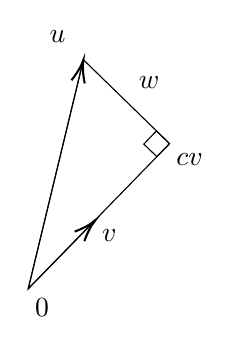
\begin{tikzpicture}[x=0.75pt,y=0.75pt,yscale=-1,xscale=1]
	\draw   (179.23,85.99) -- (152.64,196.33) -- (220.73,126.4) -- cycle ;
	\draw   (208.32,126.61) -- (214.42,120.3) -- (220.73,126.4) -- (214.63,132.71) -- cycle ;
	\draw    (152.64,196.33) -- (178.76,87.93) ;
	\draw [shift={(179.23,85.99)}, rotate = 103.55] [color={rgb, 255:red, 0; green, 0; blue, 0 }  ][line width=0.75]    (10.93,-3.29) .. controls (6.95,-1.4) and (3.31,-0.3) .. (0,0) .. controls (3.31,0.3) and (6.95,1.4) .. (10.93,3.29)   ;
	\draw    (152.64,196.33) -- (183.61,164.7) ;
	\draw [shift={(185,163.27)}, rotate = 134.39] [color={rgb, 255:red, 0; green, 0; blue, 0 }  ][line width=0.75]    (10.93,-3.29) .. controls (6.95,-1.4) and (3.31,-0.3) .. (0,0) .. controls (3.31,0.3) and (6.95,1.4) .. (10.93,3.29)   ;
	\draw (154.64,199.73) node [anchor=north west][inner sep=0.75pt]    {$0$};
	\draw (187,166.67) node [anchor=north west][inner sep=0.75pt]    {$v$};
	\draw (222.73,129.8) node [anchor=north west][inner sep=0.75pt]    {$cv$};
	\draw (161.73,70.8) node [anchor=north west][inner sep=0.75pt]    {$u$};
	\draw (204.73,92.8) node [anchor=north west][inner sep=0.75pt]    {$w$};
	\end{tikzpicture}
	\end{center}
	The idea is the find $c,w\st\langle v,w\rangle=0$ and $w=u-cv$. That is, $u=w+cv$. Since $\langle v,w\rangle=0$, then we have \[\langle v,u-cv\rangle=0=\langle u-cv,v\rangle=\langle u,v\rangle-c\|v\|^2.\] So, \[c=\dfrac{\langle u,v\rangle}{\|v\|^2}\] and \[w=u-cv=u-\dfrac{\langle u,v\rangle}{\|v\|^2}v.\]
\end{prf}
\begin{thm}{Cauchy-Schwarz Inequality}
	Suppose $u,v\in V$. Then, \[\qty|\langle u,v\rangle|\leq\|u\|\|v\|.\]	This inequality is an equality if and only if one of $u,v$ is a scalar multiples of the other. 
\end{thm}
\begin{prf}
	If $v=0$, then $\qty|\langle u,v\rangle|=0=\|u\|\|v\|$. So, we can assume $v\neq0$. Consider the orthogonal decomposition, \[u=\dfrac{\langle u,v\rangle}{\|v\|^2}\cdot v+w.\]	Then, by the Pythagorean Theorem, we have \[\begin{aligned}\|u\|^2=\left\|\dfrac{\langle u,v\rangle}{\|v\|^2}\cdot v\right\|^2+\|w\|^2&=\dfrac{\qty|\langle u,v\rangle|^2}{\|v\|^4}\|v\|^2+\|w\|^2\\&=\dfrac{\qty|\langle u,v\rangle|^2}{\|v\|^2}+\|w\|^2\geq\dfrac{\qty|\langle u,v\rangle|^2}{\|v\|^2}\end{aligned}\] As $\|v\|^2>0$, we have $\|u\|^2\|v\|^2\geq\qty|\langle u,v\rangle|^2$. Further since $\|u\|\geq0,\ \|v\|\geq0$, and $\qty|\langle u,v\rangle|\geq0$, then \[\qty|\langle u,v\rangle|\leq\|u\|\|v\|.\] The equality holds if and only if $\|w\|^2=0$. That is, $w=0$ from the orthogonal decomposition. In other words, $u$ and $v$ are linearly dependent. 
\end{prf}
\begin{thm}{Triangle Inequality}
		Suppose $u,v\in V$. Then \[\|u+v\|\leq\|u\|+\|v\|.\] This inequality is an equality if and only if one of $u,v$ is a non-negative multiple of the other. 
\end{thm}
\begin{prf}
	Note that \[\begin{aligned}\|u+v\|^2&=\langle u+v,u+v\rangle\\&=\langle u,u\rangle+\langle u,v\rangle+\langle v,u\rangle+\langle v,v\rangle\\&=\langle u,u\rangle+\langle v,v\rangle+\langle u,v\rangle+\overline{\langle u,v\rangle}\\&=\|u\|^2+\|v\|^2+2\Re\qty(\langle u,v\rangle)\\&\leq\|u\|^2+\|v\|^2+2\qty|\langle u,v\rangle|\\&\leq\|u\|^2+\|v\|^2+2\|u\|\|v\|&\text{Cauchy-Schwarz Inequality}\\&=\qty(\|u\|+\|v\|)^2.\end{aligned}\] Since $\|u+v\|\geq0,\ \|u\|\geq0,$ and $\|v\|\geq0$, we have \[\|u+v\|\leq\|u\|+\|v\|.\] The equality holds if and only if $\langle u,v\rangle=\|u\|\|v\|$. That is, when $u$ and $v$ are linearly dependent to each other. 
\end{prf}
\begin{rmk}
	After proving this triangle inequality, we finally, and officially, complete our proof to show the norm induced by an inner product as stated in Definition 5.1.10 is indeed a norm satisfying the formal definition of norms as stated in Definition 5.1.9.	
\end{rmk}
\begin{thm}{Parallelogram Equality}
	Suppose $u,v\in V$. Then \[\|u+v\|^2+\|u-v\|^2=2\qty(\|u\|^2+\|v\|^2).\]
\end{thm}
\begin{prf}
	Note that \[\begin{aligned}\|u+v\|^2+\|u-v\|^2&=\langle u+v,u+v\rangle+\langle u-v,u-v\rangle\\&=\langle u,u\rangle+\langle v,v\rangle+\langle u,v\rangle+\langle v,u\rangle+\langle u,u\rangle+\langle v,v\rangle-\langle u,v\rangle-\langle v,u\rangle\\&=\|u\|^2+\|u\|^2+\|v\|^2+\|v\|^2\\&=2\qty(\|u\|^2+\|v\|^2).\end{aligned}\]	
\end{prf}
\begin{thm}{}
	Suppose $V$ is a real inner product space. Then, \[\langle u,v\rangle=\dfrac{\|u+v\|^2-\|u-v\|^2}{4}.\]	
\end{thm}
\begin{prf}
	Note that \[\begin{aligned}\|u+v\|^2-\|u-v\|^2&=\langle u+v,u+v\rangle-\langle u-v,u-v\rangle\\&=\|u\|^2+\|v\|^2+2\langle u,v\rangle-\qty(\|u\|^2+\|v\|^2-2\langle u,v\rangle)\\&=4\langle u,v\rangle.\end{aligned}\] So, we have \[\langle u,v\rangle=\dfrac{\|u+v\|^2-\|u-v\|^2}{4}.\]
\end{prf}
\begin{thm}{}
	Suppose $V$ is a complex inner product space. Then, \[\langle u,v\rangle=\dfrac{\|u+v\|^2-\|u-v\|^2+\|u+\i v\|^2\i-\|u-\i v\|^2\i}{4}.\]	
\end{thm}
\begin{prf}
	Note that \[\begin{aligned}&\langle u+v,u+v\rangle-\langle u-v,u-v\rangle+\langle u+\i v,u+\i v\rangle\i-\langle u-\i v,u-\i v\rangle\i\\&=2\langle u,v\rangle+2\langle v,u\rangle+\qty(2\langle u,\i v\rangle+2\langle\i v,u\rangle)\i\\&=2\langle u,v\rangle+2\langle v,u\rangle+\qty(-2\i\langle u,v\rangle+2\i\langle v,u\rangle)\i\\&=2\langle u,v\rangle+2\langle v,u\rangle+2\langle u,v\rangle-2\langle v,u\rangle\\&=4\langle u,v\rangle.\end{aligned}\] so, we have \[\langle u,v\rangle=\dfrac{\|u+v\|^2-\|u-v\|^2+\|u+\i v\|^2\i-\|u-\i v\|^2\i}{4}.\]	
\end{prf}
\begin{thm}{}
	Let $U$ be a vector space. If $\|\ \|$ is a norm on $U$ satisfying the parallelogram equality, then there is an inner product $\langle\ \rangle$ on $U\st\|u\|=\sqrt{\langle u,u\rangle}\quad\forall u\in U.$
\end{thm}

\newpage
\subsection{Orthonormal Bases}
\begin{df}{Orthonormal}
	A list of vectors is called \textit{orthonormal} if each vector in the list has norm $1$ and is orthogonal to all the other vectors in the list. In other words, a list $e_1,\cdots,e_m$ of vectors in $V$ is orthonormal if \[\langle e_j,e_k\rangle=\begin{cases}1\quad\text{if }j=k\\0\quad\text{if }j\neq k\end{cases}.\]	
\end{df}
\begin{thm}{}
	If $e_1,\cdots,e_m$ is an orthonormal list of vectors in $V$, then \[\|a_1e_1+\cdots+a_me_m\|^2=\qty|a_1|^2+\cdots+\qty|a_m|^2\quad\forall a_1,\cdots,a_m\in\F.\]	
\end{thm}
\begin{prf}
	Note that \[\langle a_1e_1,a_2e_2+\cdots+a_me_m\rangle=\langle a_1e_1,a_2e_2\rangle+\cdots+\langle a_1e_1,a_me_m\rangle=0.\] So, by the Pythagorean Theorem, we have \[\begin{aligned}\|a_1e_1+\cdots+a_me_m\|^2&=\|a_1e_1\|^2+\|a_2e_2+\cdots+a_me_m\|^2\\&=\|a_1e_1\|^2+\|a_2e_2\|^2+\cdots+\|a_me_m\|^2\\&=|a_1|^2+|a_2|^2+\cdots+|a_m|^2.\end{aligned}\]
\end{prf}
\begin{thm}{}
	Every orthonormal list of vectors is $\LI$.
\end{thm}
\begin{prf}
	Suppose $e_1,\cdots,e_m$ is an orthonormal list of vectors in $V$. Then, $\|a_1e_1+\cdots+a_me_m\|^2=0$. By Theorem 5.2.2, it is equivalent to $|a_1|^2+\cdots+|a_m|^2=0$. Since each $|a_j|\geq0$, it must be $a_j=0$ for all $j=1,\cdots,m$. Therefore, the orthonormal list is $\LI$.
\end{prf}
\begin{df}{Orthonormal Basis}
	An \textit{orthonormal basis} of $V$c is an orthonormal list of vectors in $V$ that is also a basis of $V$.	
\end{df}
\begin{thm}{}
	Every orthonormal list of vectors in $V$ with length $\dim V$c is an orthonormal basis of $V$.
\end{thm}
\begin{prf}
	By Theorem 5.2.3, any orthonormal list of vectors must be $\LI$. Further since it has length $\dim V$, it is a basis of $V$. So, by definition, it is an orthonormal basis of $V$.	
\end{prf}
\begin{thm}{}
	Suppose $e_1,\cdots,e_n$ is an orthonormal basis of $V$ and $v\in V$. Then, $v=\langle v,e_1\rangle e_1+\cdots+\langle v,e_n\rangle e_n$, and $\|v\|^2=|\langle v,e_1\rangle|^2+\cdots+|\langle v,e_n\rangle|^2.$
\end{thm}
\begin{prf}
	Suppose $v\in V$ and $v=a_1e_1+\cdots+a_ne_n$. Then, \[\langle v,e_j\rangle=\langle a_1e_1+\cdots+a_ne_n,e_j\rangle=\langle a_je_j,e_j\rangle=a_j.\] So, we have \[v=\langle v,e_1\rangle e_1+\cdots+\langle v,e_n\rangle e_n.\] Further, by Theorem 5.2.2, we have \[\|v\|^2=|\langle v,e_1\rangle|^2+\cdots+|\langle v,e_n\rangle|^2.\]	
\end{prf}
\begin{thm}{Gram-Schmidt Procedure}
	Suppose $v_1,\cdots,v_m$ is $\LI$ list of vectors in $V$. Let $e_1=\dfrac{v_1}{\|v_1\|}$. For $j=2,\cdots,m$, define $e_j$ inductively by \begin{equation}\label{eq15}e_j=\dfrac{v_j-\langle v_j,e_1\rangle e_1-\cdots-\langle v_j,e_{j-1}\rangle e_{j-1}}{\|v_j-\langle v_j,e_1\rangle e_1-\cdots-\langle v_j,e_{j-1}\rangle e_{j-1}\|}.\end{equation} Then, $e_1,\cdots,e_m$ is an orthonormal list of vectors in $V\st\span(v_1,\cdots,v_j)=\span(e_1,\cdots,e_j)$ for $j=1,\cdots,m$.
\end{thm}
\begin{prf}
	To prove that Gram-Schmidt Procedure indeed produces an orthonormal list of vectors in $V$, we will use prove by mathematical induction. \par
	$\boxed{\text{Base Case}}$	Suppose $j=1$, then $\span(v_1)=\span(e_1)$ since $v_1$ is a positive multiple of $e_1$. So, the conclusion holds when $j=1$. \par 
	$\boxed{\text{Inductive Steps}}$ Suppose for some $1<j<m$, we have $\span(v_1,\cdots,v_{j-1})=\span(e_1,\cdots,e_{j-1})$. Since$v_1,\cdots,v_m$ is $\LI$, we know $v_j\notin\span(v_1,\cdots,v_{j-1})$. That is, $v_j\notin\span(e_1,\cdots,e_{j-1})$. (\textit{If $v_j\in\span(e_1,\cdots,e_{j-1}),$ then $v_j=\langle v_j,e_1\rangle e_1+\cdots+\langle v_j,e_{j-1}\rangle e_{j-1}$.) Then, we are dividing by $0$ in Equation (\ref{eq15}).} So, we are not dividing by $0$ in Equation (\ref{eq15}). Dividing a vector by its norm produces a new vector with norm $1$, so $\|e_j\|=1$. Now, we want to verify $e_j$ is orthogonal to $e_1,\cdots,e_{j-1}$. Pick some $k\st 1\leq k<j$. Then \[\begin{aligned}\langle e_j,e_k\rangle &=\left\langle\dfrac{v_j-\langle v_j,e_1\rangle e_1-\cdots-\langle v_j,e_{j-1}\rangle e_{j-1}}{\|v_j-\langle v_j,e_1\rangle e_1-\cdots-\langle v_j,e_{j-1}\rangle e_{j-1}\|}, e_k\right\rangle\\&=\dfrac{\langle v_j-\langle v_j,e_1\rangle e_1-\cdots-\langle v_j,e_{j-1}\rangle e_{j-1}, e_k\rangle}{\|\langle v_j-\langle v_j,e_1\rangle e_1-\cdots-\langle v_j,e_{j-1}\rangle e_{j-1}\|}\\&=\dfrac{\langle v_j,e_k\rangle - \langle v_j,e_k\rangle}{\|\langle v_j-\langle v_j,e_1\rangle e_1-\cdots-\langle v_j,e_{j-1}\rangle e_{j-1}\|}\\&=0\end{aligned}\] Then, $e_1,\cdots,e_j$ is an orthonormal basis, and $v_j\in\span(e_1,\cdots,e_j)$ since $v_j$ is a linear combination of $e_1,\cdots,e_j$ by Equation (\ref{eq15}). Further, we have \[\dim\span(v_1,\cdots,v_j)=\dim\span(e_1,\cdots,e_j)\] and \[\span(v_1,\cdots,v_j)\subseteq\span(e_1,\cdots,e_j).\] That is, exactly, $\span(v_1,\cdots,v_j)=\span(e_1,\cdots,e_j).$
\end{prf}
\begin{thm}{}
	Every $\FD$ inner product space has an orthonormal basis.	
\end{thm}
\begin{prf}
	Suppose $V$ is $\FD$, and select a basis of $V$. Apply Gram-Schmidt Procedure (Theorem 5.2.7) to this basis, we then have an orthonormal basis of $V$.	
\end{prf}
\begin{thm}{}
	Suppose $V$ is $\FD$. Then, every orthonormal list of vectors in $V$ can be extended to an orthonormal basis of $V$.	
\end{thm}
\begin{prf}
	Suppose $e_1,\cdots,e_m$ is an orthonormal list of vectors in $V$. Then, $e_1,\cdots,e_m$ is $\LI$ and can be extended to a basis $e_1,\cdots,e_m,v_1,\cdots,v_n$ of $V$. Apply Gram-Schmidt Procedure to this basis, we get an orthonormal list $e_1,\cdots,e_m,f_1,\cdots,f_n$. Here, $e_1,\cdots,e_m$ is unchanged since they are already orthonormal. Then, $e_1,\cdots,e_m,f_1,\cdots,f_n$ is an orthonormal basis of $V$.
\end{prf}
\begin{thm}{}
		Suppose $T\in\L(V)$. If $T$ has an upper-triangular matrix with respect to some basis of $V$, then $T$ has an upper-triangular matrix with respect to some orthonormal basis of $V$.
\end{thm}
\begin{prf}
	Suppose $\M(T)$ is upper-triangular with respect to a basis $v_1,\cdots,v_n$ of $V$. Then, we know $\span(v_1,\cdots,v_j)$ is invariant under $T$ for $j=1,\cdots,n$. Apply Gram-Schmidt Procedure to $v_1,\cdots,v_n$, we will get an orthonormal basis $e_1,\cdots,e_n$ of $V$. Further, since $\span(e_1,\cdots,e_j)=\span(v_1,\cdots,v_j)$ for $j=1,\cdots,n$, we know $\span(e_1,\cdots,e_j)$ is invariant under $T$. Therefore, $T$ has an upper-triangular matrix with respect to the orthonormal basis $e_1,\cdots,e_n$.	
\end{prf}
\begin{thm}{Schur's Theorem}
	Suppose $V$ is a $\FD$ complex vector space and $T\in\L(V)$. Then, $T$ has an upper-triangular matrix with respect to some orthonormal basis of $V$.	
\end{thm}
\begin{prf}
	Since $V$ is a $\FD$ complex vector space, $T$ must have an upper-triangular matrix with respect to some basis of $V$. Further, by Theorem 5.2.10, $T$ must have an upper-triangular matrix with respect to an orthonormal basis of $V$.	
\end{prf}
\begin{eg}{}
	The function $\phi:\F^3\to\F$ defined by \[\phi(z_1,z_2,z_3)=2z_1-5z_2+z_3\] is a linear functional on $\F^3$. We could write this linear functional in the form $\phi(z)=\langle z,u\rangle$ for every $z\in\F^3$, where $u=\langle2,-5,1\rangle$.	
\end{eg}
\begin{thm}{Riesz Representation Theorem}
	Suppose $V$ is $\FD$ and $\phi$ is a linear functional on $V$. Then, there is a unique vector $u\in V\st \phi(v)=\langle v,u\rangle$ for every $v\in V$.	
\end{thm}
\begin{prf}
	Let $e_1,\cdots,e_n$ be an orthonormal basis of $V$. Then, for all $v\in V$, we have \[v=\langle v,e_1\rangle e_1+\cdots+\langle v,e_n\rangle e_n.\] So, \[\begin{aligned}\phi(v)&=\phi(\langle v,e_1\rangle e_1+\cdots+\langle v,e_n\rangle e_n)\\&=\langle v,e_1\rangle\phi(e_1)+\cdots+\langle v,e_n\rangle\phi(e_n)\\&=\langle v,\overline{\phi(e_1)}e_1\rangle+\cdots+\langle v,\overline{\phi(e_n)}e_n\rangle\\&=\langle v,\overline{\phi(e_1)}e_1+\cdots+\overline{\phi(e_n)}e_n\rangle.\end{aligned}\] Suppose $\exists u_1,u_2\in V\st\phi(v)=\langle v,u_1\rangle=\langle v,u_2\rangle$. Then, $\langle v,u_1\rangle-\langle v,u_2\rangle=\langle v,u_1-u_2\rangle=0$. Let $v=u_1-u_2$, then we have $\langle u_1-u_2,u_1-u_2\rangle=0$. So, it must be $u_1=u_2$. Therefore, $\exists$ a unique $u\in V$ and \[u=\overline{\phi(e_1)}e_1+\cdots+\overline{\phi(e_n)}e_n\st\phi(v)=\langle v,u\rangle\quad\forall v\in V.\]
\end{prf}
\begin{eg}{}
	Find $u\in\P_2(\R)\st\dsst\int_{-1}^1p(t)(\cos(\pi t))\ \d t=\int_{-1}^1p(t)u(t)\ \d t$ for every $p\in\P_2(\R)$.
	\begin{rmk} Define an inner product on $\P_2(\R)$ as $\langle p,q\rangle=\dsst\int_{-1}^1p(x)q(x)\ \d x$ to solve this problem.\end{rmk}
	\begin{sol}
		Let $\phi\in\L(\P_2(\R),\R)$ be defined as $\phi(t)=\dsst\int_{-1}^1p(t)(\cos(\pi t))\ \d t$. Note that $1,x,x^2$ is a basis of $\P_2(\R)$. To find an orthonormal basis of $\P_2(\R)$, apply Gram-Schmidt Procedure, we have \[e_1=\dfrac{1}{\|1\|}=\dfrac{1}{\sqrt{\dsst\int_{-1}^11\cdot1\ \d t}}=\sqrt{\dfrac{1}{2}}.\] Since $x-\langle x,e_1\rangle e_1=x-\dsst\int_{-1}^1x\sqrt{\dfrac{1}{2}}\ \d x\cdot\sqrt{\dfrac{1}{2}}=x$, and $\|x\|=\sqrt{\dsst\int_{-1}^1x^2\ \d x}=\sqrt{\dfrac{2}{3}}$, we have \[e_2=\dfrac{x}{\sqrt{\dfrac{2}{3}}}=\sqrt{\dfrac{3}{2}}x.\] Further, consider \[\begin{aligned}x^2-\langle x^2,e_1\rangle e_1-\langle x^2,e_2\rangle e_2&=x^2-\dsst\int_{-1}^1x^2\sqrt{\dfrac{1}{2}}\ \d x\cdot\sqrt{\dfrac{1}{2}}-\int_{-1}^1x^2\sqrt{\dfrac{3}{2}}x\ \d x\cdot\sqrt{\dfrac{3}{2}}x\\&=x^2-\dfrac{1}{3},\end{aligned}\] and note that \[\left\|x^2-\dfrac{1}{3}\right\|=\sqrt{\int_{-1}^1\qty(x^2-\dfrac{1}{3})^2\ \d x}=\sqrt{\int_{-1}^1x^4-\dfrac{2}{3}x^2+\dfrac{1}{9}\ \d x}=\sqrt{\dfrac{8}{45}}.\] So, we have \[e_3=\dfrac{\ \ \ x^2-\dfrac{1}{3}\ \ \ }{\sqrt{\dfrac{8}{45}}}=\sqrt{\dfrac{45}{8}}\qty(x^2-\dfrac{1}{3}).\] That is, $e_1=\sqrt{\dfrac{1}{2}},\ e_2=\sqrt{\dfrac{3}{2}}x,\ e_3=\sqrt{\dfrac{45}{8}}\qty(x^2-\dfrac{1}{3})$ is an orthonormal basis of $\P_2(\R)$. Then, we have \[\phi(e_1)=\int_{-1}^1\sqrt{\dfrac{1}{2}}\cos(\pi t)\ \d t=\sqrt{\dfrac{1}{2}}\int_{-1}^1\cos(\pi t)\ \d t=0\] \[\phi(e_2)=\int_{-1}^1\sqrt{\dfrac{3}{2}}t\cos(\pi t)\ \d t=\sqrt{\dfrac{3}{2}}\int_{-1}^1t\cos(\pi t)\ \d t=0\] \[\begin{aligned}\phi(e_3)&=\int_{-1}^1\sqrt{\dfrac{45}{8}}\qty(t^2-\dfrac{1}{3})\cos(\pi t)\ \d t\\&=\sqrt{\dfrac{45}{8}}\int_{-1}^1t^2\cos(\pi t)\ \d t-\sqrt{\dfrac{45}{8}}\cdot\dfrac{1}{3}\underbrace{\int_{-1}^1\cos(\pi t)\ \d t}_0\\&=\sqrt{\dfrac{45}{8}}\int_{-1}^1t^2\cos(\pi t)\ \d t\\&=\sqrt{\dfrac{45}{8}}\qty(-\dfrac{4}{\pi^2}).\end{aligned}\] So, by Theorem 5.2.15 and its proof, we know \[\begin{aligned} u=\phi(e_1)e_1+\phi(e_2)e_2+\phi(e_3)e_3&=0+0+\sqrt{\dfrac{45}{8}}\qty(-\dfrac{4}{\pi^2})\sqrt{\dfrac{45}{8}}\qty(x^2-\dfrac{1}{3})\\&=\dfrac{45}{8}\qty(-\dfrac{4}{\pi^2})\qty(x^2-\dfrac{1}{3})\\&=-\dfrac{45}{2\pi^2}\qty(x^2-\dfrac{1}{3}).\end{aligned}\]
	\end{sol}
\end{eg}

\newpage
\subsection{Orthogonal Complements and Minimization Problems}
\begin{df}{Orthogonal Complement, $U^\perp$}
	If $U$ is a subset of $V$, then the \textit{orthogonal complement} of $U$, denoted $U^\perp$, is the set of all vectors in $V$ that are orthogonal to every vector in $U$: \[U^\perp=\qty{v\in v\mid\langle v,u\rangle=0\quad\forall u\in U}.\]	
\end{df}
\begin{thm}{Basic Properties of Orthogonal Complements}
	\begin{enumerate}
		\item If $U$ is a subset of $V$, then $U^\perp$ is a subspace of $V$.
		\item $\qty{0}^\perp=V$.
		\item $V^\perp=\qty{0}$.
		\item If $U$ is a subset of $V$, then $U\cap U^\perp\subseteq\qty{0}$.
		\item If $U$ and $W$ are subsets of $V$ and $U\subseteq W$, then $W^\perp\subseteq U^\perp$.
	\end{enumerate}	
\end{thm}
\begin{prf}
	\begin{enumerate}
		\item Let $v,w\in U^\perp$. Then $\langle v+w,u\rangle=\langle v,w\rangle+\langle w,u\rangle=0+0=0$. So, $v+w\in U^\perp$. Further, suppose $\lambda\in\F$. Then $\langle\lambda v,u\rangle=\lambda\langle v,u\rangle=\lambda\cdot0=0$. So, $\lambda v\in U^\perp$. Finally since $\langle0,u\rangle=0$, we know $0\in U^\perp$. Then, $U^\perp$ is a subspace of $V$.$\pqde$
		\item Since $\langle v,0\rangle=0\quad\forall v\in V$, we know $\qty{0}^\perp=V$. $\pqde$
		\item Suppose $v\in V^\perp$. Then, $\langle v,v\rangle=0$. By property of an inner product, it must be that $v=0$. So, $V^\perp=\qty{0}$. $\pqde$
		\item Suppose $U$ is a subset of $V$. Let $v\in U\cap U^\perp$. Then, $v\in U$ and $v\in U^\perp$. So, $\langle v,v\rangle=0$. Then, it must be that $v=0$. So, $U\cap U^\perp\subseteq\qty{0}$. $\pqde$
		\item Suppose $U$ and $W$ are subsets of $V$ with $U\subseteq W$. Suppose $v\in W^\perp$. Then, $\langle v,u\rangle=0\quad\forall u\in W$. Since $U\subseteq W$, we have $\langle v,w\rangle=0\quad\forall u\in U$. That is, $v\in U^\perp$. Then, we have $W^\perp\subseteq U^\perp$.
	\end{enumerate}	
\end{prf}
\begin{thm}{}
	Suppose $U$ is a $\FD$ subspace of $V$. Then, $V=U\oplus U^\perp$.	
\end{thm}
\begin{prf}
	Suppose $u\in U$ and $w\in U^\perp$. Then, $\forall v\in V$, we have $v=cu+w$ for some $c\in\F$ and $\langle u,w\rangle=0$. Then, we have $V=U+U^\perp$. Further, by Theorem 5.3.2(4), $U\cap U^\perp=\qty{0}$ since $U$ and $U^\perp$ are all subspaces of $V$. Hence, $V=U\oplus U^\perp$.
\end{prf}
\begin{cor}{}
	Suppose $V$ is $\FD$ and $U$ is a subspace of $V$. Then, $\dim U^\perp=\dim V-\dim U.$	
\end{cor}
\begin{thm}{}
	Suppose $U$ is a $\FD$ subspace of $V$. Then, $U=(U^\perp)^\perp$.	
\end{thm}
\begin{prf}
	\par ($\subseteq$). Suppose $u\in U$. Then, $\langle u,v\rangle=0\quad\forall v\in U^\perp$. Then, $u\in(U^\perp)^\perp$. That is, $U\subseteq(U^\perp)^\perp.\pqde$	
	\par ($\supseteq$). Suppose $v\in(U^\perp)^\perp$. Then, $v=u+w$ for some $u\in U$ and $w\in U^\perp$. Then, $w=v-u\in(U^\perp)^\perp$. Since $U\subseteq(U^\perp)^\perp$, we know $u\in U^\perp$. Then, $v-u\in(U^\perp)^\perp$. Hence, $v-u\in U^\perp\cap(U^\perp)^\perp$. That is, $v-u$ is orthogonal to itself. So, it must be that $v-u=0$ or $v=u$. Since $u\in U$ and $v\in U$, we have shown that $(U^\perp)^\perp\subseteq U$.
\end{prf}
\begin{df}{Orthogonal Projection, $P_U$}
	Suppose $U$ is a $\FD$ subspace of $V$. Then orthogonal projection of $V$ onto $U$ is the operator $P_U\in\L(V)$ defined as follows: For $v\in V$, write $v=u+w$, where $u\in U$ and $w\in U^\perp$. Then, $P_Uv=u$.	
\end{df}
\begin{rmk} By Theorem 5.3.3, $V=U\oplus U^\perp$, which ensures each $v\in V$ can be uniquely represented in the form of $u+w$ with $u\in U$ and $w\in U^\perp$, and thus $P_U$ is well-defined.\end{rmk}
\begin{eg}{}
	Suppose $x\in V$ with $x\neq0$ and $U=\span(x)$. Show that \[P_Uv=\dfrac{\langle v,x\rangle}{\|x^2\|}x\qquad\forall v\in V.\]
	\begin{prf}
		Suppose $v\in V$. Then, \[v=\dfrac{\langle v,x\rangle}{\|x^2\|}x+\qty(v-\dfrac{\langle v,x\rangle}{\|x^2\|}x),\] where $\dfrac{\langle v,x\rangle}{\|x^2\|}x\in\span(x)$ and $v-\dfrac{\langle v,x\rangle}{\|x^2\|}x\in U^\perp$. Thus, $P_Uv=\dfrac{\langle v,x\rangle}{\|x^2\|}x$.
	\end{prf}	
\end{eg}
\begin{thm}{Properties of Orthogonal Projections}
	Suppose $U$ is a $\FD$ subspace of $V$ and $v\in V$. Then, 
	\begin{enumerate}
		\item $P_U\in\L(V)$.
		\item $P_Uu=u\quad\forall u\in U$.
		\item $P_Uw=0\quad\forall w\in U^\perp$.
		\item $\range P_U=U$.
		\item $\Null P_U=U^\perp$.
		\item $v-P_Uv\in U^\perp$.
		\item $P_U^2=P_U$.
		\item $\|P_Uv\|\leq\|v\|$.
		\item for every orthonormal basis $e_1,\cdots,e_m$ of $U$, \[P_Uv=\langle v,e_1\rangle e_1+\cdots+\langle v,e_m\rangle e_m.\]
	\end{enumerate}	
\end{thm}
\begin{prf}
	\begin{enumerate}
		\item Suppose $v_1=u_1+w_1$ and $v_2=u_2+w_2$, where $v_1,v_2\in V$, $u_1,u_2\in U$, and $w_1,w_2\in U^\perp$. Then, $v_1+v_2=(u_1+u_2)+(w_1+w_2)$, where $u_1+u_2\in U$ and $w_1+w_2\in U^\perp$. So, \[P_U(v_1+v_2)=u_1+u_2=P_Uv_1+P_Uv_2.\] Additionally, suppose $\lambda\in\F$. Then, $\lambda v_1=\lambda u_1+\lambda w_1$, where $\lambda u_1\in U$ and $\lambda w_1\in U^\perp$. Then, \[P_U(\lambda v_1)=\lambda u_1=\lambda P_U(v_1).\pqde\]
		\item Suppose $u\in U$. Then, $u=u+0$, where $u\in U$ and $0\in U^\perp$. So, $P_Uu=u.\pqde$
		\item Suppose $w\in U^\perp$. Then, $w=0+w$, where $0\in U$ and $w\in U^\perp$. So, $P_Uw=0.\pqde$
		\item By definition of $P_U$, we have $\range P_U\subseteq U$. By Theorem 5.3.8(2), we know $U\subseteq\range P_U$. So, $\range P_U=U.\pqde$
		\item By Theorem 5.3.8(3), we have $U^\perp\subseteq\Null P_U$. Further note if $v\in\Null P_U$, then $v=0+v$ with $0+u$ and $v\in U^\perp$. So, $\Null P_U\subseteq U^\perp$. That is, $\Null P_U=U.\pqde$
		\item If $v=u+w$ with $u\in U$ and $w\in U^\perp$, then \[v-P_Uv=v-u=w\in U^\perp.\pqde\]
		\item If $v=u+w$ with $u\in U$ and $w\in U^\perp$, then \[(P_U^2)v=P_U(P_Uv)=P_Uu=u=P_Uv.\] So, $P_U^2=P_U.\pqde$
		\item If $v=u+w$ with $u\in U$ and $w\in U^\perp$, then we have \[\|P_Uv\|^2=\|u\|^2\leq\|u\|^2+\|w\|^2=\|v\|^2\] by the Pythagorean Theorem. $\pqde$
		\item If $v=u+w$ with $u\in U$ and $w\in U^\perp$, then \[v=u+w=\langle v,e_1\rangle e_1+\cdots+\langle v,e_m\rangle e_m+\qty(v-\langle v,e_1\rangle e_1-\dots-\langle v,e_m\rangle e_m).\] Since $e_1,\cdots,e_m$ is an orthonormal basis of $U$, we have $\langle ve_1\rangle e_1+\cdots+\langle v,e_m\rangle e_m\in U$. Now, consider \[\begin{aligned}\big\langle\langle v,e_1\rangle e_1+\cdots+\langle v,e_m\rangle e_m,v-\langle v,e_1\rangle e_1-\cdots-\langle v,e_m\rangle e_m\big\rangle&=\big\langle\langle v,e_1\rangle e_1+\cdots+\langle v,e_m\rangle e_m,v\big\rangle-\|u\|^2\\&=\langle v,e_1\rangle\langle e_1,v\rangle+\cdots+\langle v,e_m\rangle\langle e_m,v\rangle-\|u\|^2\\&=\langle v,e_1\rangle\overline{\langle v,e_1\rangle}+\cdots+\langle v,e_m\rangle\overline{\langle v,e_m\rangle}-\|u\|^2\\&=\qty|\langle v,e_1\rangle|^2+\cdots+\qty|\langle v,e_m\rangle|^2-\|u\|^2\\&=\|u\|^2-\|u\|^2=0\quad (By\ Theorem\ 5.2.2)\end{aligned}\] Then, $v-\langle v,e_1\rangle e_1-\cdots-\langle v,e_m\rangle e_m\in U^\perp$. So, we have $P_Uv=\langle v,e_1\rangle e_1+\cdots+\langle v,e_m\rangle e_m.$
	\end{enumerate}	
\end{prf}
\begin{thm}{Minimizing the Distance to a Subspace}
	Suppose $U$ is a $\FD$ subspace of $V$, $v\in V$, and $u\in U$. Then, $\|v-P_Uv\|\leq\|v-u\|$. The inequality is an equality if and only if $u=P_Uv$.
\end{thm}
\begin{prf}
	Note that $\|v-P_Uv\|^2\leq\|v-P_Uv\|^2+\|P_Uv-u\|^2$ since $\|P_Uv-u\|^2\geq0$. Further, since $v-P_Uv\in U^\perp$ by Theorem 5.3.8(6) and $P_Uv-u\in U$ by the Pythagorean Theorem, we have \[\|v-P_Uv\|^2+\|P_Uv-u\|^2=\|v=P_Uv+P_Uv-u\|^2=\|v-u\|^2.\] Then, $\|u-P_Uv\|^2\leq\|v=P_Uv\|^2+\|P_Uv-u\|^2=\|v-u\|^2$. Since $\|v-P_Uv\|^2\geq0$ and $\|v-u\|^2\geq0$, we have $\|v-P_Uv\|\leq\|v-u\|$. The equality holds if and only  if $\|P_Uv-u\|^2=0$. That is, $\|P_Uv-u\|=0$, $P_Uv-u=0$, or $P_Uv=u$.
\end{prf}
\begin{eg}{}
	In $\R^4$, set $U=\span((1,1,0,0),(1,1,1,2))$. Find $u\in U\st\|u-(1,2,3,4)\|$ is as small as possible.
	\begin{sol}
		By Theorem 5.3.9, we need to find $P_Uv=\langle v,e_1\rangle e_1+\langle v,e_2\rangle e_2$. Thus, we need to use Gram-Schmidt Procedure to find $e_1$ and $e_2$: \[e_1=\dfrac{1}{\sqrt{2}}(1,1,0,0)\qquad\text{and}\qquad e_2=\dfrac{1}{\sqrt{5}}(0,0,1,2).\] Set $v=(1,2,3,4)$, we have \[\begin{aligned}P_Uv&=\langle(1,2,3,4),\dfrac{1}{\sqrt{2}}(1,1,0,0)\rangle\dfrac{1}{\sqrt{2}}(1,1,0,0)+\langle(1,2,3,4),\dfrac{1}{\sqrt{5}}(0,0,1,2)\rangle\dfrac{1}{\sqrt{5}}(0,0,1,2)\\&=\qty(\dfrac{3}{2},\dfrac{3}{2},\dfrac{11}{5},\dfrac{22}{5}).\end{aligned}\]	
	\end{sol}
	
\end{eg}


\newpage
\section{Operators on Inner Product Spaces}
\subsection{Self-Adjoint and Normal Operators}
\begin{df}{Adjoint, $T^*$}
	Suppose $T\in\L(V,W)$. The \textit{adjoint} of $T$ is the function $T^*:W\to V\st$ \[\langle Tv,w\rangle=\langle v,T^*w\rangle\] for every $v\in V$ and every $w\in W$.
\end{df}
\begin{thm}{}
	If $T\in\L(V,W),$ then $T^*\in\L(W,V).$
\end{thm}
\begin{prf}
	\begin{enumerate}
		\item The definition of adjoint makes sense.\par Suppose $T\in\L(V,W)$. Fix $w\in W$. Let $f:V\to\F$ be defined as $v\mapsto\langle Tv,w\rangle$. Then, $f$ is a linear functional on $V$. Note that \[\begin{aligned}f(au+bv)=\langle T(au+bv),w\rangle&=\langle aTu+bTv,w\rangle\\&=a\langle Tu,w\rangle+b\langle Tv,w\rangle\\&=af(u)+b(fv).\end{aligned}\] By Riesz Representation Theorem, we know $f(v)=\langle v,\Delta\rangle$ for some $\Delta\in V$. We call this unique $\Delta$ as $T^*w$. That is, for each $w\in W$, $\exists$ unique $T^*w\in V$. So, $T^*$ is well-defined as a function from $W$ to $V$. $\pqde$
		\item Adjoint is a linear map.\par Suppose $w_1,w_2\in W$. If $v\in V$, then \[\begin{aligned}\langle v,T^*(w_1+w_2)\rangle=\langle Tv,w_1+w_2\rangle&=\langle Tv,w_1\rangle+\langle Tv,w_2\rangle\\&=\langle v,T^*w_1\rangle+\langle v,T^*w_2\rangle\\&=\langle v,T^*w_1+T^*w_2\rangle.\end{aligned}\] So, $T^*(w_1+w_2)=T^*w_1+T^*w_2.\pqde$\par Now fix $w\in W$ and $\lambda\in\F$. If $v\in V$, then \[\begin{aligned}\langle v,T^*(\lambda w)\rangle=\langle Tv,\lambda w\rangle&=\overline{\lambda}\langle Tv,w\rangle\\&=\overline{\lambda}\langle v,T^*w\rangle\\&=\langle v,\lambda T^*w\rangle.\end{aligned}\] So, we know $T^*(\lambda w)=\lambda T^*w.\pqde$\par Thus, we've shown $T^*$ is a linear map as desired. 
	\end{enumerate}	
\end{prf}
\begin{eg}
	Define $T:\R^3\to\R^2$ by $T(x_1,x_2,x_3)=(x_2+3x_3,2x_1)$. Find a formula for $T^*$.
	\begin{sol}
		Define $T^*:\R^2\to\R^3$. Let $y=(y_1,y_2)\in\R^2$. Then, \[\begin{aligned}\langle x,T^*y\rangle=\langle Tx,y\rangle&=y_1x_2+3y_1x_3+2x_1y_2\\&=\langle(x_1,x_2,x_3),(2y_2,y_1,3y_1)\rangle.\end{aligned}\] Thus, $T^*:\R^2\to\R^3$ is defined as $T^*(y_1,y_2)=(2y_2,y_1,3y_1).$
	\end{sol}
\end{eg}
\begin{eg}
	Fix $u\in V$ and $x\in W$. Define $T\in\L(V,W)$ by $Tv=\langle v,u\rangle x$ for every $v\in V$. Find a formula for $T^*$.
	\begin{sol}
		Define $T^*\in\L(W,V)$. Consider \[\begin{aligned}\langle v,T^*w\rangle=\langle Tv,w\rangle&=\big\langle\langle v,u\rangle x,w\big\rangle\\&=\langle v,u\rangle\langle x,w\rangle\\&=\big\langle v,\langle w,x\rangle u\big\rangle.\end{aligned}\] So, we have $T^*w=\langle w,x\rangle u$.
	\end{sol}
\end{eg}
\begin{thm}{Properties of the Adjoint}
	\begin{enumerate}
		\item $(S+T)^*=S^*+T^*\quad\forall S,T\in\L(V,W)$.
		\item $(\lambda T)^*=\overline{\lambda}T^*\quad\forall\lambda\in\F$ and $T\in\L(V,W)$.
		\item $(T^*)^*=T\quad\forall T\in\L(V,W)$.
		\item $I^*=I$, where $I$ is the identity operator on $V$.
		\item $(ST)^*=T^*S^*\quad\forall T\in\L(V,W)$ and $S\in\L(W,U)$.
	\end{enumerate}	
\end{thm}
\begin{prf}
	\begin{enumerate}
		\item Consider \[\begin{aligned}\langle v,(S+T)^*w\rangle=\langle(S+T)v,w\rangle&=\langle Sv,w\rangle+\langle Tv,w\rangle\\&=\langle v,S^*w\rangle+\langle v,T^*w\rangle\\&=\langle v,S^*w+T^*w\rangle\\&=\langle v,(S^*+T^*)w\rangle.\end{aligned}\] So, we have $(S+T)^*w=(S^*+T^*)w\quad\forall w\in W.\pqde$
		\item Note that \[\begin{aligned}\langle v,(\lambda T)^*w\rangle=\langle(\lambda T)v,w\rangle&=\lambda\langle Tv,w\rangle\\&=\lambda\langle v,T^*w\rangle\\&=\langle v,\overline{\lambda}T^*w\rangle.\end{aligned}\] So, we get $(\lambda T)^*w=\overline{\lambda}T^*w\quad\forall w\in W.\pqde$
		\item Consider \[\begin{aligned}\langle v,(T^*)^*w\rangle=\langle T^*v,w\rangle&=\overline{\langle w,T^*v\rangle}\\&=\overline{\langle Tw,v\rangle}\\&=\langle v,Tw\rangle.\end{aligned}\] So, it is $(T^*)^*w=Tw\quad\forall w\in W.\pqde$
		\item Note we have \[\langle v,I^*w\rangle=\langle Iv,w\rangle=\langle v,w\rangle.\] So, $I^*w=w\quad\forall w\in W$. That is, $I^*=I.\pqde$
		\item We have \[\begin{aligned}\langle v,(ST)^*w\rangle=\langle(ST)v,w\rangle&=\langle S(Tv),w\rangle\\&=\langle Tv,S^*w\rangle\\&=\langle v,T^*(S^*w)\rangle.\end{aligned}\]So, $(ST)^*w=T^*(S^*w)=(T^*S^*)w\quad\forall w\in W.$
	\end{enumerate}	
\end{prf}
\begin{thm}{Null Space and Range of $T^*$}
	Suppose $T\in\L(V,W)$. Then, 
	\begin{enumerate}
		\item $\Null T^*=(\range T)^\perp$.
		\item $\range T=(\null T^*)^\perp$.
		\item $\Null T=(\range T^*)^\perp$.
		\item $\range T^*=(\Null T)^\perp$.
	\end{enumerate}
\end{thm}
\begin{prf}
	\begin{enumerate}
		\item Suppose $w\in\Null T^*$. Then, $T^*w=0$. So, $\langle v,T^*w\rangle=0$. That is, $\langle Tv,w\rangle=0\quad\forall v\in0$. Then, $w$ is orthogonal to any $Tv$. That is, $w\in(\range T)^\perp$. Conversely, if $w\in(\range T)^\perp$, we have $\langle Tv,w\rangle=0$, and thus $\langle v,T^*w\rangle=0,$ or $T^*w=0$. That is, $w\in\Null T^*$. Hence, $\Null T^*=(\range T)^\perp.\pqde$
		\item Note that $(\Null T^*)^\perp=\qty(\qty(\range T)^\perp)^\perp=\range T.\pqde$
		\item Suppose $v\in\Null T$. Then, $Tv=0,$ and $\langle Tv,w\rangle=0$. So, $\langle v,T^*w\rangle=0\quad\forall w\in W$. Then, $v$ is orthogonal to every vectors in $T^*w$. So, $v\in\qty(\range T^*)^\perp$. In the other way around, if we assume $v\in\qty(\range T^*)^\perp$, then $\langle v,T^*w\rangle=\langle Tv,w\rangle=0$. So, $Tv=0$, and thus $v\in\Null T$. Hence, we have $\Null T=\qty(\range T^*)^\perp.\pqde$
		\item Consider $(\Null T)^\perp=\qty((\range T^*)^\perp)^\perp=\range T^*$.
	\end{enumerate}	
\end{prf}
\begin{df}{Conjugate Transpose}
	The \textit{conjugate transpose} of an $m\times n$ matrix is the $n\times m$ matrix obtained by interchanging the rows and columns and then taking the conjugate of each entry. 	
\end{df}
\begin{thm}{}
	Let $T\in\L(V,W)$. Suppose $e_1,\cdots,e_n$ is an orthonormal basis of $V$ and $f_1,\cdots,f_m$ is an orthonormal basis of $W$. Then, $\M\qty(T^*,(f_1,\cdots,f_m),(e_1,\cdots,e_m))$ is the conjugate transpose of $\M\qty(T,(e_1,\cdots,e_n),(f_1,\cdots,f_m))$.
\end{thm}
\begin{prf}
	Suppose $\M(T)$ denote the matrix $\M\qty(T,(e_1,\cdots,e_n),(f_1,\cdots,f_m))$ and let $\M(T^*)$ denote the matrix $\M\qty(T^*,(f_1,\cdots,f_m),(e_1,\cdots,e_m))$. Then, note that $Te_k=\langle Te_k,f_1\rangle f_1+\cdots+\langle Te_k,f_m\rangle f_m$. So, \[\qty(\M(T))_{j,k}=\langle Te_k,f_j\rangle.\] Further, consider $T^*f_k=\langle T^*f_k,e_1\rangle e_1+\cdots+\langle T^*f_k,e_n\rangle e_n$. That is, \[\begin{aligned}\qty(\M(T^*))_{j,k}=\langle T^*f_k,e_j\rangle&=\overline{\langle e_j,T^*f_k\rangle}\\&=\overline{\langle Te_j,f_k\rangle}\\&=\overline{\qty(\M(T))_{k,j}}\end{aligned}\] So, we've shown that $\M(T^*)$ is the conjugate transpose of $\M(T)$.
\end{prf}
\begin{df}{Self-Adjoint}
	An operator $T\in\L(V)$ is called \textit{self-adjoint} if $T=T^*$. In other words, $T\in\L(V)$ is self-adjoint if and only if $\langle Tv,w\rangle=\langle v,Tw\rangle\quad\forall v,w\in V$.	
\end{df}
\begin{thm}{}
	The sum of two self-adjoint operators is self-adjoint, and the product of a real scalar and a self-adjoint operator is self-adjoint. 	
\end{thm}
\begin{prf}
	\begin{enumerate}
		\item Suppose $T,S\in\L(V)$ are self-adjoint. Then, \[(S+T)^*=S^*+T^*=S+T.\] So, $S+T$ is self-adjoint. $\pqde$
		\item Let $\lambda\in\R$. Then, \[(\lambda T)^*=\lambda T^*=\lambda T.\] So, $\lambda T$ is self-adjoint. 
	\end{enumerate}	
\end{prf}
\begin{thm}{}
	Every eigenvalue of a self-adjoint operator is real.	
\end{thm}
\begin{prf}
	Suppose $T$ is a self-adjoint operator on $V$. Let $\lambda$ be an eigenvalue of $T$, and let $v$ be a non-zero vector in $V\st Tv=\lambda v$. Then, \[\lambda\|v\|^2=\langle\lambda v,v\rangle=\langle Tv,v\rangle=\langle v,Tv\rangle=\langle v,\lambda v\rangle=\overline{\lambda}\|v\|^2.\] So, it must be $\lambda=\overline{\lambda}$, which means $\lambda$ is real.
\end{prf}
\begin{thm}{}
	Suppose $V$ is a complex inner product space and $T\in\L(V)$. Suppose $\langle Tv,v\rangle=0\quad\forall v\in V$. Then, $T=0$.	
\end{thm}
\begin{prf}
	Note that \[\begin{aligned}\langle Tu,w\rangle&=\dfrac{1}{4}\qty\Big[\big\langle T(u+w),u+w\big\rangle-\big\langle T(u-w),u-w\big\rangle]\\&\qquad+\dfrac{\i}{4}\qty\Big[\big\langle T(u+\i w),u+\i w\big\rangle-\big\langle T(u-\i w),(u-\i w)\big\rangle]\\&=0\quad\forall u,w\in V.\end{aligned}\] Let $w=Tu\in V$. Then, $\langle Tu,Tu\rangle=0$. That is, $Tu=0\quad\forall u\in V$. So, $T=0$.
\end{prf}
\begin{thm}{}
	Suppose $V$ is a complex inner product space and $T\in\L(V)$. Then, $T$ is self-adjoint if and only if $\langle Tv,v\rangle\in\R\quad\forall v\in V$.	
\end{thm}
\begin{prf}
	\par ($\Rightarrow$) Let $v\in V$. Then, \begin{equation}\label{eq16}\begin{aligned}\langle Tv,v\rangle-\overline{\langle Tv,v\rangle}&=\langle Tv,v\rangle-\langle v,Tv\rangle\\&=\langle Tv,v\rangle-\langle T^*v,v\rangle\\&=\langle (T-T^*)v,v\rangle\end{aligned}\end{equation} If $\langle Tv,v\rangle\in\R\quad\forall v\in V$, then Equation (\ref{eq16})$=0$. That is, $\langle (T-T^*)v,v\rangle=0\quad\forall v\in V$. So, $T-T^*=0,$ or $T=T^*$. That is, $T$ is self-adjoint. $\pqde$
	\par ($\Leftarrow$)	Conversely, if $T$ is self-adjoint, then Equation (\ref{eq16})$=0$. That is, $\langle Tv,v\rangle=\overline{\langle Tv,v\rangle}=0$, or we have $\langle Tv,v\rangle=\overline{\langle Tv,v\rangle}$. This is equivalent to the conclusion $\langle Tv,v\rangle\in\R$.
\end{prf}
\begin{thm}{}
	Suppose $T$ is a self-adjoint operator on $V\st\langle Tv,v\rangle=0\quad\forall v=V$. Then, $T=0$.	
\end{thm}
\begin{prf}
	We've already shown this to be true under a complex inner product space. Thus, we can assume $V$ is a real inner product space. If $u,w\in V$, then \[\begin{aligned}\langle Tu,w\rangle&=\dfrac{1}{4}\langle T(u+w),u+w\rangle-\langle T(u-w),u-w\rangle\\&=0\quad\forall u,w\in V.\end{aligned}\]	Let $w=Tu$. Then, $\langle Tu,Tu\rangle=0$, or $Tu=0\quad\forall u\in V$. So, $T=0$.
\end{prf}
\begin{df}{Normal Operator}
	An operator on an inner product space is called \textit{normal} if it commutes with its adjoint. In other words, $T\in\L(V)$ is normal if $TT^*=T^*T$.	
\end{df}
\begin{eg}
	Let $T$ be the operator on $\F^2$ whose matrix with respect to the standard basis is \[\mqty(2&-3\\3&2).\] Show that $T$ is not self-adjoint but is still normal.
	\begin{prf}
		Since $\M(T)=\mqty(2&-3\\3&2)$ and $\M(T^*)=\mqty(2&3\\-3&2),$ then $\M(T)\neq\M(T^*),$ and thus it is not self-adjoint. However, note that \[\mqty(2&-3\\3&2)\mqty(2&3\\-3&2)=\mqty(13&0\\0&13)\] and \[\mqty(2&3\\-3&2)\mqty(2&-3\\3&2)=\mqty(13&0\\0&13).\] So, by definition, $T$ is normal. 
	\end{prf}
\end{eg}
\begin{thm}{}
	An operator $T\in\L(V)$ is normal if and only if $\|Tv\|=\|T^*v\|\quad\forall v\in V$.	
\end{thm}
\begin{prf}
	Note that \[\begin{aligned}T\text{ is normal}&\iff T^*T-TT^*=0\\&\iff\big\langle(T^*T-TT^*)v,v\big\rangle=0\quad\forall v\in V\\&\iff\langle T^*Tv,v\rangle=\langle TT^*v,v\rangle\quad\forall v\in V\\&\iff\langle Tv,Tv\rangle=\langle T^*v,T^*v\rangle\quad\forall v\in V\\&\iff\|Tv\|^2=\|T^*v\|^2\quad\forall v\in V.\end{aligned}\] Since $\|Tv\|\geq0$ and $\|T^*v\|\geq0$, it is equivalent to \[\|Tv\|=\|T^*v\|\quad\forall v\in V.\]	
\end{prf}
\begin{thm}{}
	Suppose $T\in\L(V)$ is normal and $v\in V$ is an eigenvector of $T$ with eigenvalue $\lambda$. Then, $v$ is also an eigenvector of $T^*$ with eigenvalue $\overline{\lambda}$.	
\end{thm}
\begin{prf}
	Note that $(T-\lambda I)^*=T^*-\overline{\lambda}I$. Consider $(T-\lambda I)(T-\lambda I)^*=TT^*-\overline{\lambda}T-\lambda T^*+\lambda\overline{\lambda}$ and $(T-\lambda I)^*(T-\lambda I)=T^*T-\overline{\lambda}T-\lambda T^*+\lambda\overline{\lambda}$. Since, $T$ is normal, $TT^*=T^*T$. So. \[(T-\lambda I)(T-\lambda I)^*=(T-\lambda I)^*(T-\lambda I).\] That is, $T-\lambda I$ is also normal. So, by Theorem 6.1.17, we have \[\|(T-\lambda I)v\|=\|(T^*-\overline{\lambda}I)v\|=0.\] That is, $T^*v=\overline{\lambda}v$, or $v$ is an eigenvector of $T^*$ with eigenvalue $\overline{\lambda}$.
\end{prf}
\begin{thm}{}
	Suppose $T\in\L(V)$ is normal. Then, eigenvectors of $T$ corresponding to distinct eigenvalues are orthogonal.	
\end{thm}
\begin{prf}
	Suppose $\alpha,\beta$ are distinct eigenvalues of $T$, with corresponding eigenvectors $u,v$. Then, $Tu=\alpha u$ and $Tv=\beta v$. By Theorem 6.1.18, we have $T^*v=\overline{\beta}v$. So, we have \[\begin{aligned}(\alpha-\beta)\langle u,v\rangle&=\langle\alpha u,v\rangle-\langle u,\overline{\beta}v\rangle\\&=\langle Tu,v\rangle-\langle U,T^*v\rangle\\&=\langle Tu,v\rangle-\langle Tu,v\rangle\\&=0.\end{aligned}\] Since $\alpha\neq\beta$, it must be $\langle u,v\rangle=0$. So, $u$ and $v$ are orthogonal. 
\end{prf}

\newpage
\subsection{The Spectral Theorem}
\begin{thm}{Complex Spectral Theorem}
	Suppose $\F=\C$ and $T\in\L(V)$. Then, the following are equivalent: 
	\begin{enumerate}
		\item $T$ is normal.
		\item $V$ has an orthonormal basis consisting of eigenvectors of $T$.
		\item $T$ has a diagonal matrix with respect to some orthonormal basis of $V$.
	\end{enumerate}
\end{thm}
\begin{prf}
	Note that ($2$)$\iff$($3$) is obvious by Theorem 4.3.5. No we need to show ($3$)$\iff$($1$) to complete the proof. $\pqde$\par 
	Suppose ($3$). Then, $\M(T)$ is diagonal. That is, $\M(T^*)$ is also diagonal. Then, $\M(T)\M(T^*)=\M(T^*)\M(T)$. That is $\M(TT^*)=\M(T^*T)$, or $TT^*=T^*T$. So, $T$ is normal. $\pqde$\par 
	Suppose ($1$). That is, $T$ is normal. Then, by Schur's Theorem, $\exists$ an orthonormal basis $e_1,\cdots,e_n$ of $V\st\M(T,(e_1,e_n))$ is an upper triangular matrix. Suppose \[\M(T,(e_1,\cdots,e_n))=\mqty(a_{1,1}&\cdots&a_{1,n}\\&\ddots&\vdots\\0&&a_{n,n}).\] Then, \[\M(T^*,(e_1,\cdots,e_n))=\mqty(\overline{a_{1,1}}&&0\\\vdots&\ddots&\\\overline{a_{1,n}}&\cdots&\overline{a_{n,n}}).\] Then, $Te_1=a_{1,1}e_1$ and $T^*e_1=\overline{a_{1,1}}e_1+\cdots+\overline{a_{1,n}}e_n$. Further, note that $\|Te_1\|^2=\qty|a_{1,1}|^2$ and $\|T^*e_1\|^2=\qty|a_{1,1}|^2+\cdots+\qty|a_{1,n}|^2$. Since $\|Te_1\|^2=\|T^*e_1\|^2$, we have $\qty|a_{1,1}|^2=\qty|a_{1,1}|^2+\cdots+\qty|a_{1,n}|^2$. Then, it must be that $\qty|a_{1,2}|^2+\cdots+\qty|a_{1,n}|^2=0$. Applying this procedure to $\|Te_2\|^2=\|T^*e_2\|^2,\cdots,\|Te_n\|^2=\|T^*e_n\|^2$, we have $|a_{j,k}|=0$ when $j\neq k$. So, $\M(T)$ is a diagonal matrix. 
\end{prf}
\begin{lem}{Invertible Quadratic Expressions}
	Suppose $T\in\L(V)$ is self-adjoint and $b,c\in\R$ are $\st b^2<4c$. Then, $T^2+bT+cI$ is invertible.	
\end{lem}
\begin{prf}
	Let $v\in V\st v\neq0$. Note that \[\begin{aligned}\langle(T^2+bT+cI)v,v\rangle&=\langle T^2v,v\rangle+b\langle Tv,v\rangle+c\langle v,v\rangle\\&=\langle Tv,Tv\rangle+b\langle Tv,v\rangle+c\|v\|^2&T\ is\ self-adjoint\\&\geq\|Tv\|^2-\qty|b|\|Tv\|\|v\|+c\|v\|^2&Cauchy-Schwarz\\&=\qty(\|Tv\|-\dfrac{\qty|b|\|v\|}{2})^2+\qty(c-\dfrac{b^2}{4})\|v\|^2\\&>0&b^2<4c\end{aligned}\] Then, $\forall v\neq0,\ \langle(T^2+bT+cI)v,v\rangle>0$. So, it must be that $(T^2+bT+cI)v=0$ if and only if $v=0$. Then, $\Null(T^2+bT+cI)=\qty{0}$. Thus, $T^2+bT+cI$ is injective, and thus it is invertible.
\end{prf}
\begin{lem}{}
	Suppose $V\neq\qty{0}$ and $T\in\L(V)$ is a self-adjoint operator. Then, $T$ has an eigenvalue. 	
\end{lem}
\begin{prf}
	Let $m=\dim V$ and choose $v\in V$. Then, $v,Tv,\cdots,T^nv$ cannot be $\LI$ because we have $n+1>\dim V$ vectors in the list. So, $\exists a_0,\cdots,a_n\in\R\st a_0v+a_1Tv+\cdots+a_nT^nv=0$. Make the $a$'s the coefficient of a polynomial then \[a_0+a_1x+\cdots+a_nx^n=c(x^2+b_1x+c_1)\cdots(x^2+b_Mx+c_M)(x-\lambda_1)\cdots(x-\lambda_m),\] where $c$ is a non-zero real number, each $b_j,c_j,\lambda_j\in\R$, each $b_j<4c_j$, and $m+M\geq1$. Then, we have \[\begin{aligned}0&=a_0v+a_1Tv+\cdots+a_nT^nv\\&=(a_0I+a_1T+\cdots+a_nT^n)v\\&=c(T^2+b_1T+c_1I)\cdots(T^2+b_MT+c_MI)(T-\lambda_1I)\cdots(T-\lambda_mI).\end{aligned}\] By Lemma 6.2.2,  $T^2+b_jT+c_jI$ is invertible. Since $c\neq0$, it must be that $0=(T-\lambda_1I)\cdots(T-\lambda_mI)$. Hence, $T-\lambda_jI$ is not injective for at least one $j$. So, $T$ has at least one eigenvalue. 
\end{prf}
\begin{df}{Restriction Operator, $T|_U$}
	Suppose $T\in\L(V)$ and $U$ is an invariant subspace of $V$ under $T$. Then, the \textit{restriction operator}, $T|_U\in\L(V)$, is defined as $T|_U(u)=Tu$ for $u\in U$.
\end{df}
\begin{thm}{}
	Suppose $T\in\L(V)$ is self-adjoint and $U$ is a subspace of $V$ that is invariant under $T$. Then, 
	\begin{enumerate}
		\item $U^\perp$ is invariant under $T$;
		\item $T|_U\in\L(U)$ is self-adjoint;
		\item $T|_{U^\perp}\in\L(U^\perp)$ is self-adjoint. 
	\end{enumerate}	
\end{thm}
\begin{prf}
	\begin{enumerate}
		\item Suppose $v\in U^\perp$ and $u\in U$. Then, $\langle v,Tu\rangle=\langle Tv,u\rangle=0$ since $U$ is invariant under $T$ (and hence $Tu\in U$) and $v\in U^\perp$. Then, we have $Tv\in U^\perp\quad\forall v\in U^\perp$, proving $U^\perp$ is an invariant subspace under $T.\pqde$
		\item Note that if $u,v\in U$, then \[\langle(T|_U)u,v\rangle=\langle Tu,v\rangle=\langle u,Tv\rangle=\langle u,(T|_U)v\rangle.\] Therefore, $T|_U$ is self-adjoint. $\pqde$
		\item Replace $U$ with $U^\perp$ in ($2$) and apply the conclusion from ($1$), and we complete the proof.
	\end{enumerate}
\end{prf}
\begin{thm}{Real Spectral Theorem}
	Suppose $\F=\R$ and $T\in\L(V)$. Then, the following are equivalent: 
	\begin{enumerate}
		\item $T$ is self-adjoint;
		\item $V$ has an orthonormal basis consisting of eigenvectors of $T$.
		\item $T$ has a diagonal matrix with respect to some orthonormal basis of $V$.
	\end{enumerate}
\end{thm}
\begin{prf}
	Similar to the complex case, ($2$)$\iff$($3$) is obvious. So, we will show ($3$)$\implies$($1$) and ($1$)$\implies$($2$) to complete the proof. $\pqde$\par 
	Suppose ($3$) holds. Then, $\M(T)$ is diagonal. So, we have $\M(T)^t=\M(T)$. That is, $T=T^*$, and thus $T$ is self-adjoint. $\pqde$\par 
	Suppose ($1$) holds. We will use mathematical induction on $\dim V$. $\boxed{\text{Base Case}}$ When $\dim V=1$. Clearly, ($1$)$\implies$($2$). $\boxed{\text{Inductive Steps}}$ Assume $\dim V>1$ and ($1$)$\implies$($2$) holds for all cases with dimension $\dim V-1$. Let $u$ be an eigenvector of $T$ with $\|u\|=1$. Let $U=\span(u)$. Then, $\dim U=1$. Since $V=U\oplus U^\perp$, we know $\dim U^\perp=\dim V-\dim U=\dim V-1$. So, ($1$)$\implies$($2$) holds on $U^\perp$. That is, $\exists$ an orthonormal basis of $U^\perp$ consisting of eigenvectors of $T|_{U^\perp}$. Now, add $u$ to this orthonormal basis, we get a basis of $V$. Further since $u\in U$, this basis is an orthonormal basis of $V$ consisting of eigenvectors of $T$. 
\end{prf}

\newpage
\subsection{Positive Operators and Isometries}
\begin{df}{Positive Operator}
	An operator $T\in\L(V)$ is called \textit{positive} if $T$ is self-adjoint and $\langle Tv,v\rangle\geq0\quad\forall v\in V$.	
\end{df}
\begin{df}{Square Root}
	An operator $R$ is called a \textit{square root} of an operator $T$ if $R^2=T$.	
\end{df}
\begin{eg}
	Suppose $T\in\L(\R^3)$ and $R\in\L(\R^3)$ be defined as $T(z_1,z_2,z_3)=(z_3,0,0)$ and $R(z_1,z_2,z_3)=(z_2,z_3,0)$. Then, $R$ is a square root of $T$.
	\begin{prf}
		Since $R^2(z_1,z_2,z_3)=R(z_2,z_3,0)=(z_3,0,0)=T(z_1,z_2,z_3)$, $R$ is a square root of $T$.
	\end{prf}	
\end{eg}
\begin{thm}{Characterization of Positive Operators}
	Let $T\in\L(V)$. Then, the following are equivalent: 
	\begin{enumerate}
		\item $T$ is positive;
		\item $T$ is self-adjoint and all the eigenvalues of $T$ are non-negative;
		\item $T$ has a positive square root;
		\item $T$ has a self-adjoint square root;
		\item $\exists$ an operator $R\in\L(V)\st T=R^*R$.
	\end{enumerate}	
\end{thm}
\begin{prf}
	\par ($1$)$\implies$($2$): Since $T$ is positive, then $T$ is self-adjoint. Let $\lambda$ be an eigenvalue of $T$. Then, $Tv=\lambda v$ for some $v\in V$. Then, $\langle Tv,v\rangle=\langle\lambda v,v\rangle=\lambda\langle v,v\rangle=\lambda\|v\|^2$. Since $T$ is positive, $\langle Tv,v\rangle\geq0$. Further since $\|v\|^2\geq0$, it must also be $\lambda\geq0$. So, we complete the proof. $\pqde$\par 
	($2$)$\implies$($3$): Suppose $T$ is self-adjoint and all the eigenvalues of $T$ are non-negative. By the Spectrum Theorem, $\exists$ an orthonormal basis $e_1,\cdots,e_n$, where $e_1,\cdots,e_n$ are eigenvectors of $T$. Let $\lambda_1,\cdots,\lambda_n$ be the corresponding eigenvalues, where $\lambda_j\geq0$. Let $R\in\L(V)\st Re_j=\sqrt{\lambda_j}e_j$. Then \[\begin{aligned}\langle Rv,v\rangle&=\Big\langle a_1\sqrt{\lambda_1}e_1+\cdots+a_n\sqrt{\lambda_n}e_n,a_1e_1+\cdots+a_ne_n\Big\rangle\\&=\qty|a_1|^2\sqrt{\lambda_1}+\cdots+\qty|a_n|^2\sqrt{\lambda_n}\geq0.\end{aligned}\] Further, we can verity $R$ is self-adjoint (proof omitted). So, $R$ is positive by definition. Note that \[R^2e_j=R\qty(\sqrt{\lambda_j}e_j)=\sqrt{\lambda_j}\sqrt{\lambda_j}e_j=\lambda_je_j=Te_j.\] So, $R$ is a square root of $T$. $\pqde$\par 
	($3$)$\implies$($4$): Suppose $T$ has a positive square root. By definition, positive operators are self-adjoint. $\pqde$\par 
	($4$)$\implies$($5$): Suppose $T$ has a self-adjoint square root. Then, we have $R\in\L(V)\st R^*=R$ and $R^2=T$. That is, $T=R^2=RR=R^*R.\pqde$\par 
	($5$)$\implies$($1$): Suppose $\exists$ an operator $R\in\L(V)\st T=T^*T$. Then, \[T^*=\qty(R^*R)^*=R^*\qty(R^*)^*=R^*R=T.\] So, $T$ is self-adjoint. Now, since \[\langle Tv,v\rangle=\langle R^*Rv,v\rangle=\langle Rv,Rv\rangle=\|Rv\|^2\geq0,\] we have $T$ is a positive operator. 
\end{prf}
\begin{thm}{}
	Each positive operator on $V$ has a unique positive square root.	
\end{thm}
\begin{prf}
	Let $T$ be a positive operator on $V$. Select $v$ to be an eigenvector of $T$ with corresponding eigenvalue of $\lambda$. Then, we have $Tv=\lambda v$. Let $R$ be a positive square root of $T$. Apply Spectrum Theorem to $R$, then $\exists$ an orthonormal basis $e_1,\cdots,e_n$, where $e_1,\cdots,e_n$ are eigenvectors of $R$. Then, $\exists\lambda_1,\cdots,\lambda_n\geq0\st Re_j=\sqrt{\lambda_j}e_j$. Suppose $v\in V$ and $v=a_1e_1+\cdots+a_ne_n$. Then, \[Rv=a_1\sqrt{\lambda_1}e_1+\cdots+a_n\sqrt{\lambda_n}e_n\quad\text{and}\quad R^2v=a_1\lambda_1e_1+\cdots+a_n\lambda_ne_n.\] Further, $Tv=\lambda v=\lambda a_1e_1+\cdots+\lambda a_ne_n$. Since $R^2v=Tv$, we know \[a_1\qty(\lambda_1-\lambda)e_1+\cdots+a_n\qty(\lambda_n-\lambda)e_n=0.\] Since $e_1,\cdots,e_n$ is an orthonormal basis, for each $j=1,\cdots,n$, we have $a_j(\lambda_j-\lambda)=0$. So, it must be $a_j=0$ or $\lambda_j=\lambda$. If $a_j=0$, then we can delet it from the representation of $v$. So, \[v=\sum_{\qty{j\mid\lambda_j=\lambda}}a_je_j\] Hence, \[Rv=\sum_{\qty{j\mid\lambda_j=\lambda}}a_j\sqrt{\lambda}e_j=\sqrt{\lambda}v.\]
\end{prf}
\begin{df}{Isometry}
	An operator $S\in\L(V)$ is called an \textit{isometry} if $\|Sv\|=\|v\|\quad\forall v\in V$. In other words, an operator is an isometry if ti preserves norms. 	
\end{df}
\begin{eg}
	Let $\lambda_1,\cdots,\lambda_n\in\F$ with $\qty|\lambda_j|$ and $S\in\L(V)\st Se_j=\lambda_je_j$ for some orthonormal bases $e_1,\cdots,e_n$ of $V$. Then, $S$ is an isometry. 
	\begin{prf}
		Let $v\in V$. Then, $v=\langle v,e_1\rangle e_1+\cdots+\langle v,e_n\rangle e_n$. So, $\|v\|^2=\qty|\langle v,e_1\rangle|^2+\cdots+\qty|\langle v,e_n\rangle|^2$. Further, $Sv=\lambda_1\langle v,e_1\rangle e_1+\cdots+\lambda_n\langle v,e_n\rangle e_n,$ and thus $\|Sv\|^2=\qty|\lambda_1|^2\qty|\langle v,e_1\rangle|^2+\cdots+\qty|\lambda_n|^2\qty|\langle v,e_n\rangle|^2$. Since $\qty|\lambda_j|=1$, we know \[\|Sv\|^2=\qty|\langle v,e_1\rangle|^2+\cdots+\qty|\langle v,e_n\rangle|^2=\|v\|^2.\] So, $\|Sv\|=\|v\|$ since $\|Sv\|\geq0$ and $\|v\|\geq0$. That is, by definition, $S$ is an isometry. 
	\end{prf}
\end{eg}
\begin{thm}{Characterization of Isometries}
	Suppose $S\in\L(V)$. Then, the following are equivalent: 
	\begin{enumerate}
		\item $S$ is an isometry.
		\item $\langle Su,Sv\rangle=\langle u,v\rangle\quad\forall u,v\in V$;
		\item $Se_1,\cdots,Se_n$ is orthonormal for every orthonormal list of vectors $e_1,\cdots,e_n$ in $V$;
		\item $\exists$ an orthonormal basis $e_1,\cdots,e_n$ of $V\st Se_1,\cdots,Se_n$ is orthonormal;
		\item $S^*S=I$;
		\item $SS^*=I$;
		\item $S^*$ is an isometry;
		\item $S$ is invertible and $S^{-1}=S^*$.
	\end{enumerate}	
\end{thm}
\begin{prf}
	\par ($1$)$\implies$($2$): Note that \[\begin{aligned}\langle Su,Sv\rangle=\dfrac{\|Su+Sv\|^2-\|Su-Sv\|^2}{4}&=\dfrac{\|S(u+v)\|^2-\|S(u-v)\|^2}{4}\\&=\dfrac{\|u+v\|^2-\|u-v\|^2}{4}\\&=\langle u,v\rangle\pqde\end{aligned}\]	
	\par ($2$)$\implies$($3$): We have \[\langle Se_i,Se_j\rangle=\langle e_i,e_j\rangle=\begin{cases}1\quad\text{if }i=j\\0\quad\text{if }i\neq j\end{cases}\] So, $Se_1,\cdots,Se_n$ are orthonormal. $\pqde$
	\par ($3$)$\implies$($4$): Suppose $e_1,\cdots,e_m$ is orthonormal. We can extend it to a basis of $V$: $e_1,\cdots,e_m,v_{m+1},\cdots,v_n$. Then, apply the Gram-Schmidt Procedure, we get an orthonormal basis, $e_1,\cdots,e_m,e_{m+1},\cdots,e_n$ of $V$. $\pqde$
	\par ($4$)$\implies$($5$): Suppose $e_1,\cdots,e_n$ is an orthonormal basis of $V$. Then, \[\langle S^*Se_j,e_k\rangle=\langle Se_j,Se_k\rangle=\langle e_j,e_j\rangle.\] Suppose $u,v\in V\st u=a_1e_1+\cdots+a_ne_n$ and $v=b_1e_1+\cdots+b_ne_n$. Then, \[\begin{aligned}\langle S^*Su,v\rangle=\langle Su,Sv\rangle&=\langle S(a_1e_1+\cdots+a_ne_n),S(b_1e_1+\cdots+b_ne_n)\rangle\\&=\langle a_1Se_1+\cdots+a_nSe_n,b_1Se_1+\cdots+b_nSe_n\rangle\\&=\langle a_1Se_1,b_1Se_1\rangle+\cdots+\langle a_nSe_n,b_nSe_n\rangle\\&=a_1\overline{b_1}\|Se_1\|^2+\cdots+a_n\overline{b_n}\|Se_n\|^2\\&=a_1\overline{b_1}+\cdots+a_n\overline{b_n}\\&=\langle u,v\rangle.\end{aligned}\] So, $S^*Su=u$, or $S^*S=I.\pqde$
	\par ($5$)$\implies$($6$): Suppose $S^*S=I$. Then, $S=S^*$. So, $SS^*=I.\pqde$
	\par ($6$)$\implies$($7$): Suppose $S^*S=I$. Then, \[\|S^*v\|^2=\langle S^*v,S^*v\rangle=\langle SS^*v,v\rangle=\langle v,v\rangle=\|v\|^2.\pqde\]
	\par ($7$)$\implies$($8$): Suppose $S^*$ is an isometry. Then, we know $S^*S=I$ and $SS^*=I$ by the proofs done above. So, $S$ is invertible, and $S^{-1}=S^*.\pqde$
	\par ($8$)$\implies$($1$): Finally, suppose $S$ is invertible and $S^{-1}=S^*$. Then, $S^*S=I$. Note that \[\|Sv\|^2=\langle Sv,Sv\rangle=\langle S^*Sv,v\rangle=\langle v,v\rangle=\|v\|^2.\]
\end{prf}
\begin{thm}{}
	Suppose $V$ is a complex inner product space and $S\in\L(V)$. Then, $S$ is an isometry if and only if $\exists$ an orthonormal basis of $V$ consisting of eigenvectors of $S$ whose corresponding eigenvalues all have absolute value of $1$.	
\end{thm}
\begin{prf}
	\par ($\Rightarrow$): By the Spectrum Theorem, $\exists$ an orthonormal basis $e_1,\cdots,e_n$, where $e_1,\cdots,e_n$ are eigenvectors of $S$. Suppose $\lambda_1,\cdots,\lambda_n$ are the corresponding eigenvalues. Then, we have \[\|Se_j\|=\|\lambda_je_j\|=\qty|\lambda_j|.\] Since $S$ is an isometry, $\|Se_j\|=\|e_j\|=1$. So, $\qty|\lambda_j|=\|Se_j\|=1.\pqde$
	\par ($\Leftarrow$): This direction is proven in Example 6.3.7. 
\end{prf}

\newpage
\subsection{Polar Decomposition and SVD}
\begin{nota}
	If $T$ is a positive operator, then $\sqrt{T}$ denotes the unique positive square root of $T$. 
\end{nota}
\begin{rmk}We want to verify that the definition of $\sqrt{T^*T}$ is reasonable: $\langle T^*Tv,v\rangle=\langle Tv,Tv\rangle\geq0$. Also, $\qty(T^*T)^*=T^*T$. So, $T^*T$ is a positive operator, and thus $\sqrt{T^*T}$ is well-defined. \end{rmk}
\begin{thm}{Polar Decomposition}
	Suppose $T\in\L(V)$. Then, $\exists$ an isometry $S\in\L(V)\st T=S\sqrt{T^*T}$.	
\end{thm}
\begin{prf}
	\par $\boxed{\text{Step }1}$ Characteristics of $\range\sqrt{T^*T}$: Note that \[\begin{aligned}\|Tv\|^2=\langle Tv,Tv\rangle&=\langle T^*Tv,v\rangle\\&=\langle\sqrt{T^*T}\sqrt{T^*T}v,v\rangle\\&=\langle\sqrt{T^*T}v,\sqrt{T^*T}v\rangle\\&=\|\sqrt{T^*T}v\|^2.\end{aligned}\] So, $\forall v\in V$, we have $\|Tv\|=\|\sqrt{T^*T}v\|$. Define $S_1:\range\sqrt{T^*T}\to\range T$ as $S_1\qty(\sqrt{T^*T}v)=Tv$. Then, we have $\|S_1\sqrt{T^*T}v\|=\|Tv\|$.
	\begin{enumerate}
		\item Now, we want to verify that $S_1$ is well-defined. Suppose $v_1,v_2\in V\st\sqrt{T^*T}v_1=\sqrt{T^*T}v_2$. Then, \[\begin{aligned}\|Tv_1-Tv_2\|=\|T\qty(v_1-v_2)\|&=\|\sqrt{T^*T}\qty(v_1-v_2)\|\\&=\|\sqrt{T^*T}v_1-\sqrt{T^*T}v_2\|\\&=0.\end{aligned}\] So, $S_1$ is well-defined. 
		\item Further, we want to show $S_1$ is linear. By using the linearity of $T$, we can easily prove that $S_1$ is also linear.
		\item Additionally, $S_1$ is surjective by definition of $S_1$.
		\item Also, $S_1$ is isometry. Note that $\forall u\in\range\sqrt{T^*T}$, we have $\|S_1u\|=\|u\|$ since $\|\sqrt{T^*T}v\|=\|Tv\|$.
		\item Hence, $S_1$ is injective: Note that $\|S_1v\|=0$ if and only if $\|v\|=0$, which is equivalent to $v=0$. So, $\Null S_1=\qty{0}.\pqde$
	\end{enumerate}
	\par $\boxed{\text{Step }2}$ Extend $S_1$ to an isometry on $V$. Note that we have $\dim\range\sqrt{T^*T}=\dim\range T$. So, we know $\dim\qty(\range\sqrt{T^*T})^\perp=\dim\qty(\range T)^\perp$. Select an orthonormal basis $e_1,\cdots,e_m$ of $\qty(\range\sqrt{T^*T})^\perp$ and an orthonormal basis $f_1,\cdots,f_m$ of $\qty(\range T)^\perp$. Now, let's define $S_2:\qty(\range\sqrt{T^*T})^\perp\to\qty(\range T)^\perp$ as $S_1\qty(a_1e_1+\cdots+a_me_m)=a_1f_1+\cdots+a_mf_m$. We can then not only show $S_2$ is well-defined but also $S_2$ is linear. Moreover, $\forall w\in\qty(\range\sqrt{T^*T})^\perp$, if $w=a_1e_1+\cdots+a_me_m$, we have \[\begin{aligned}\|S_2w\|^2=\|S_2\qty(a_1e_1+\cdots+a_me_m)\|^2&=\|a_1f_1+\cdots+a_mf_m\|^2\\&=\qty|a_1|^2+\cdots+\qty|a_m|^2\\&=\|a_1e_1+\cdots+a_me_m\|^2\\&=\|w\|^2.\end{aligned}\] So, $\|S_2w\|=\|w\|$. Now, we define \[Sv=\begin{cases}S_1v,\quad v\in\range\sqrt{T^*T}\\S_2v,\quad v\in\qty(\range\sqrt{T^*T})^\perp\end{cases}\] Note that since $V=\range\sqrt{T^*T}\oplus\qty(\range\sqrt{T^*T})^\perp$, we can uniquely represent $v\in V$ as $v=u+w$ for some $u\in\range\sqrt{T^*T}$ and $w\in\qty(\range\sqrt{T^*T})^\perp$. Hence, we can also write the definition of $S$ as $Sv=S_1u+S_2w$. If we select $\sqrt{T^*T}v\in\range\sqrt{T^*T}$, then we have $S\qty(\sqrt{T^*T}v)=S_1\qty(\sqrt{T^*T}v)=Tv$. Therefore, $T=S\sqrt{T^*T}\quad\forall v\in V.\pqde$
	\par Finally, we will show $S$ is an isometry. Note that $v=u+w$. So, by Pythagorean Theorem, \[\begin{aligned}\|Sv\|^2=\|S_1u+S_2w\|^2&\|S_1u\|^2+\|S_2w\|^2\\&=\|u\|^2+\|w\|^2\\&=\|v\|^2.\end{aligned}\]
\end{prf}
\begin{df}{Singular Values}
	Suppose $T\in\L(V)$. The \textit{singular values} of $T$ are the eigenvalues of $\sqrt{T^*T}$, with each eigenvalue $\lambda$ repeated $\dim E\qty(\lambda,\sqrt{T^*T})$ times. 	
\end{df}
\begin{eg}
	Define $T\in\L(\F^4)$ by \[T(z_1,z_2,z_3,z_4)=(0,3z_1,2z_2,-3z_4).\] Find the singular values of $T$. 
	\begin{sol}
		Suppose $v=\qty(z_1,z_2,z_3,z_4)\in\F^4$ and $w=\qty(y_1,y_2,y_3,y_4)\in\F^4$. Consider \[\begin{aligned}\langle v,T^*w\rangle&=\langle Tv,w\rangle\\&=\langle\qty(0,3z_1,2z_2,-3z_4),\qty(y_1,y_2,y_3,y_4)\rangle\\&=3z_1\overline{y_2}+2z_2\overline{y_3}-3z_4\overline{y_4}\\&=\langle\qty(z_1,z_2,z_3,z_3),\qty(3y_2,2y_3,0,-3y_4)\rangle.\end{aligned}\] So, $T^*w=T^*\qty(y_1,y_2,y_3,y_4)=\qty(3y_2,2y_3,0,-3y_4)$. Then, $T^*T\qty(z_1,z_2,z_3,z_4)=\qty(9z_1,4z_2,0,9z_4)$. Then, $\sqrt{T^*T}\qty(z_2,z_2,z_3,z_4)=\qty(3_z1,2z_2,0,3z_4)$. So, the eigenvalues of $\sqrt{T^*T}$ are $3$, $2$, and $0$. Also, \[\dim E\qty(3,\sqrt{T^*T})=2,\quad\dim E\qty(2,\sqrt{T^*T})=\dim E\qty(0,\sqrt{T^*T})=1.\] So, the singular values are $3,3,2,0$.
	\end{sol}
\end{eg}
\begin{thm}{Singular Value Decomposition (SVD)}
	Suppose $T\in\L(V)$ has singular values $s_1,\cdots,s_n$. Then, $\exists$ orthonormal bases $e_1,\cdots,e_n$ and $f_1,\cdots,f_n$ of $V\st$ \[Tv=s_1\langle v,e_1\rangle f_1+\cdots+s_n\langle v,e_n\rangle f_n\] for every $v\in V$.
\end{thm}
\begin{rmk}Relevant Theorem used in proving SVD: Spectrum Theorem, Characterization and Properties of Isometry, and Polar Decomposition. \end{rmk}
\begin{prf}
	Apply the Spectrum Theorem to $\sqrt{T^*T}$, we know $\exists$ an orthonormal basis $e_1,\cdots,e_n$ of $V\st$\[\sqrt{T^*T}e_j=s_je_j\quad\forall j=1,\cdots,n.\] Note that $\forall v\in V$, we have \begin{equation}\label{eq17} v=\langle v,e_1\rangle e_1+\cdots+\langle v,e_n\rangle e_n\end{equation} Apply $\sqrt{T^*T}$ to Equation (\ref{eq17}) we have \begin{equation}\label{eq18} \sqrt{T^*T}v=s_1\langle v,e_1\rangle e_1+\cdots+s_n\langle v,e_n\rangle e_n.\end{equation} By Polar Decomposition, $\exists$ an isometry $S\in\L(V)\st T=S\sqrt{T^*T}$. Apply $S$ to Equation (\ref{eq18}), we get \[S\qty(\sqrt{T^*T}v)=s_1\langle v,e_1\rangle Se_1+\cdots+s_n\langle v,e_n\rangle Se_n.\] By the characteristics of isometry, since $e_1,\cdots,e_n$ is an orthonormal basis, $Se_1,\cdots,Se_n$ is also an orthonormal basis. Let $f_j=Se_j$. Then, \[Tv=S\sqrt{T^*T}v=s_1\langle v,e_e\rangle f_1+\cdots+s_n\langle v,e_n\rangle f_n.\]
\end{prf}
\begin{thm}{}
	Suppose $T\in\L(V)$. Then, the singular values of $T$ are the non-negative square roots of the eigenvalues of $T^*T$, with each eigenvalue $\lambda$ repeated $\dim E\qty(\lambda,T^*T)$ times. 	
\end{thm}
\begin{prf}
	By the Spectrum Theorem, $\exists$ an orthonormal basis $e_1,\cdots,e_n$ and non-negative number $\lambda_1,\cdots,\lambda_n\st T^*Te_j=\lambda_je_j\quad\forall j=1,\cdots,n$. Then, we have $\sqrt{T^*T}e_j=\sqrt{\lambda_j}e_j\quad\forall j=1,\cdots,n$, which completes the proof. 
\end{prf}

\newpage
\section{Operators on Complex Vector Spaces}
\subsection{Generalized Eigenvectors, Nilpotent Operators}
\begin{thm}{}
	Suppose $T\in\L(V)$. Then, \[\qty{0}\subseteq\Null T^0\subseteq\Null T^1\subseteq\cdots\subseteq\Null T^k\subseteq\Null T^{k+1}\subseteq\cdots\]	
\end{thm}
\begin{prf}
	Let $k\in\Np$. Let $v\in\Null T^k$. Then, $T^kv=0$. Then, we know $T(T^kv)=T^{k+1}v=0$. So, $v\in\Null T^{k+1}$. That is, $\Null T^k\subseteq\Null T^{k+1}$ as desired. 	
\end{prf}
\begin{thm}{}
	Suppose $T\in\L(V)$. Suppose $m$ is a non-negative integer $\st$ $\Null T^m=\Null T^{m+1}$. Then, \[\Null T^m=\Null T^{m+1}=\Null T^{m+2}=\Null T^{m+3}=\cdots\]	
\end{thm}
\begin{prf}
	Let $k\in\N$. We've already shown $\Null T^{m+k}\subseteq\Null T^{m+k+1}$ in Theorem 7.1.1. Now, let $v\in\Null T^{m+k+1}$. So, $T^{m+k+1}(v)=0$. That is, $T^{m+1}\qty(T^kv)=0$. So, $T^kv\in\Null T^{m+1}=\Null T^m$. In other words, $T^m\qty(T^kv)=T^{m+k}(v)=0$. So, $v\in\Null T^{m+k}$. Then, $\Null T^{m+k+1}\subseteq\Null T^{m+k}$. Hence, \[\Null T^{m+k}=\Null T^{m+k+1}.\]
\end{prf}
\begin{thm}{}
	Suppose $T\in\L(V)$. Let $n=\dim V$. Then, \[\Null T^n=\Null T^{n+1}=\Null T^{n+2}=\cdots\]	
\end{thm}
\begin{prf}
	Suppose for the sake of contradiction that $\Null T^n\neq\Null T^{n+1}$. Then, \[\Null T^0\nsubseteq\Null T\nsubseteq T^2\nsubseteq\cdots\nsubseteq\Null T^n\nsubseteq T^{n+1}.\] As the symbol $\nsubseteq$ means ``contained in but not equal to,'' at each of the strict inclusions in the chain above, the dimension increases by at least $1$. That is, $\dim\Null T^{n+1}\geq n+1$. $\divideontimes$ This is a contradiction because a subspace of $V$ ($\Null T^{n+1}$)	 cannot be a dimension larger than $\dim V=n$. So, it must be that our assumption is wrong, and $\Null T^n=\Null T^{n+1}$.
\end{prf}
\begin{thm}{}
	Suppose $T\in\L(V)$. Let $n=\dim V$. Then, \[V=\Null T^n\oplus\range T^n.\]	
\end{thm}
\begin{prf}
	Note that $\dim V=\dim\Null T^n+\dim\range T^n$ by the Fundamental Theorem of Linear Maps. So, we only need to prove $\qty(\Null T^n)\cap\qty(\range T^n)=\qty{0}$. Let $v\in\qty(\Null T^n)\cap\qty(\range T^n)$. Then, $\exists u\in V\st v=T^nu$. Since $v\in\Null T^n$, $T^Nv=T^n\qty(T^nu)=0$. That is, $T^{2n}u=T^nv=0$. Therefore, $u\in\Null T^{2n}=\Null T^n$. So, we now have $T^nu=0$. Hence, $v=T^nu=0$. Then, i $\qty(\Null T^n)\cap\qty(\range T^n)=\qty{0}$, and thus $V=\Null T^n\oplus\range T^n$.
\end{prf}
\begin{df}{Generalized Eigenvector}
	Suppose $T\in\L(V)$ and $\lambda$ is an eigenvalue of $T$. A vector $v\in V$ is called a \textit{generalized eigenvector} of $T$ corresponding to $\lambda$ if $v\neq0$ and $\qty(T-\lambda I)^jv=0$ for some positive integer $j$.	
\end{df}
\begin{df}{Generalized Eigenspace, $G\qty(\lambda, T)$}
	Suppose $T\in\L(V)$ and $\lambda\in\F$. The \textit{generalized eigenspace} of $T$ corresponding to $\lambda$, denoted $G\qty(\lambda, T)$, is defined to be the set of all generalized eigenvectors of $T$ corresponding to $\lambda$, along with the $0$ vector. 	
\end{df}
\begin{thm}{}
	Suppose $T\in\L(V)$ and $\lambda\in\F$. Then, \[G\qty(\lambda, T)=\Null\qty(T-\lambda I)^{\dim V}.\]	
\end{thm}
\begin{prf}
		
\end{prf}


\newpage
\subsection{Decomposition of an Operator}


\newpage
\subsection{Characteristic and Minimal Polynomials}

\newpage
\subsection{Jordan Form}

\newpage
\section{Operators on Real Vectors Spaces}
\subsection{Complexification}

\newpage
\subsection{Operators on Real Inner Product Spaces}

\newpage
\section{Trace and Determinant}
\subsection{Trace}

\newpage
\subsection{Determinant}

\newpage
\section{Exercises}
\subsection{Span and Linear Independence}
\begin{enumerate}
	\item Suppose $v_1,v_2,v_3,v_4$ spans $V$. Prove that the list $v_1-v_2,v_2-v_3,v_3-v_4,v_4$ also spans $V$.
	\item Prove that if $\C$ is a vector space on $\R$, then the list $1+\i,1-\i$ is $\LI$. 
	\item Prove that if $\C$ is a vector space on $\C$, then the list $1+\i,1-\i$ is linearly dependent.
	\item Prove or give a counterexample: Suppose $v_1,v_2,\cdots,v_m$ is $\LI$ in $V$ and $\lambda\in\F$ with $\lambda\neq0.$ Then $\lambda v_1,\lambda v_2,\cdots,\lambda v_m$ is $\LI$.
	\item Suppose $v_1,\cdots,v_m$ is $\LI$ in $V$ and $w\in V$. Prove that if $v_1+w,\cdots,v_m+w$ is linearly dependent, then $w\in\span(v_1,\cdots,v_m).$
\end{enumerate}
\subsection{Bases}
\begin{enumerate}
	\item Find all the vectors spaces that consist of only one basis. \begin{hint}$\qty{0}.$\end{hint}
	\item Suppose $U$ is a subspace of $\R^5\st U=\qty{(x_1,x_2,x_3,x_4,x_5)\in\R^5\mid x_1=3x_2,x_3=7x_4}.$ Find a basis of $U$. Extend this basis into a basis of $\R^5.$ Then, find a subspace $W$ of $\R^5\st\R^5=U\oplus W.$
	\item Suppose $v_1,v_2,v_3,v_4$ is a basis of $V$. Prove that $v_1+v_2,v_2+v_3,v_3+v_4,v_4$ is also a basis of $V$.
	\item \textbf{Prove} or disprove: $\P_3(\F)$ has a basis $p_0,p_1,p_2,p_3\st$ no one from $p_0,p_1,p_2,p_3$ has a degree of $2$. \begin{hint}Use the conclusion from \#3.\end{hint}
	\item Prove or \textbf{give a counterexample}: If $v_1,v_2,v_3,v_4$ is a basis of $V$ and $U$ is a subspace of $V\st v_1,v_2\in U,v_3\notin U,v_4\notin U,$ then $v_1,v_2$ is basis of $U$.
\end{enumerate}
\subsection{Dimension}
\begin{enumerate}
	\item Suppose $V$ is $\FD$ and $U$ is a subspace of $V\st\dim U=\dim V$. Prove that $U=V$.
	\item Prove that the subspaces of $\R^2$ are exactly the following: $\qty{0},$ $\R^2$, and all the lines passing through the origin in $\R^2$.
	\item Suppose $v_1,\cdots,v_m$ is $\LI$ in $V$ and $w\in V.$ Prove $\dim\span(v_1+w,\cdots,v_m+w)\geq m-1.$
	\item Suppose $p_0,p_1,\cdots,p_m\in\P(\F)\st \deg p_j=j$. Prove $p_0,p_1,\cdots,p_m$ is a basis of $\P_m(\F).$
	\item Suppose $U$ and $W$ are subspaces of $\R^8\st\dim U=3,\dim W=5,$ and $U+W=\R^8.$ Prove that $\R^8=U\oplus W.$
	\item Suppose $U$ and $W$ are $5$-dimensional subspaces of $\R^9.$ Prove $U\cap W\neq\qty{0}.$
	\item Suppose $U$ and $W$ are $4$-dimensional subspaces of $\C^6$. Prove that $\exists$ two vectors in $U\cap W\st$ any one of which is not a scalar multiple of another one.
	\item Suppose $U_1,\cdots,U_m$ are $\FD$ vector spaces of $V$. Prove that $U_1+\cdots+U_m$ is $\FD$ and \[\dim(U_1+\cdots+U_m)\leq\dim U_1+\cdots+\dim U_m.\]
	\item Suppose $V$ is $\FD$ and $\dim V=n\geq1.$ Prove that $\exists$ $1$-dimensional subspaces of $V$, $U_1,\cdots,U_n\st$\[V=U_1\oplus\cdots\oplus U_n.\]
	\item Suppose $U_1,\cdots,U_m$ are $\FD$ vector subspaces of $V\st U_1+\cdots+U_m$ is a direct sum. Prove that $U_1\oplus\cdots\oplus U_m$ is $\FD$ and \[\dim U_1\oplus\cdots\oplus U_m=\dim U_1+\cdots+\dim U_m.\]\begin{hint}Use mathematical induction.\end{hint}\begin{rmk}This problem deepens the analogy between direct sums of subspaces and disjoint unions of subsets. Specifically, compare this problem to the following obvious statement: if a set is written as a disjoint union of finite subsets, then the number of elements in the set equals the sum of the numbers of elements in the disjoint subsets. \end{rmk}
	\item Prove or give a counter example: \[\begin{aligned}\dim(U_1+U_2+U_3)=&\dim U_1+\dim U_2+\dim U_3\\&-\dim(U_1\cap U_2)-\dim(U_1\cap U_3)-\dim(U_2\cap U_3)\\&+\dim(U_1\cap U_2\cap U_3).\end{aligned}\] \begin{hint}Consider $U_1=\qty{(x,0)\mid x\in\R},\ U_2=\qty{(0,y)\mid y\in\R},\ U_3=\qty{(x,x)\mid x\in\R}.$\end{hint}
\end{enumerate}
\subsection{The Vector Space of Linear Maps}
\begin{enumerate}
	\item Suppose $T\in\L(V,W)$ and $v_1,\cdots,v_m$ is a vector list in $V\st Tv_1,\cdots,Tv_m$ is $\LI$ in $W$. Prove that $v_1,\cdots,v_m$ is $\LI$.
	\item Prove that $\L(V,W)$ is a vector space.
	\item Prove the algebraic properties of products of linear maps. 
	\item Show that every linear map from a $1$-dimensional vector space to itself is multiplication by some scalar. More precisely, prove that if $\dim V=1$ and $T\in\L(V,V)$, then $\exists\lambda\in\F\st Tv=\lambda v\quad\forall v\in V$.
\end{enumerate}
\subsection{Null Spaces and Range}
\begin{enumerate}
	\item Suppose $V$ is a vector space and $S,T\in\L(V,V)\st\range S\subset\Null T.$ Prove that $(ST)^2=0.$
	\item Prove that $\nexists$ a linear map $T:\R^5\to\R^5\st\range T=\Null T.$
	\item Suppose $T\in\L(V,W)$ is injective and $v_1,\cdots,v_n$ is $\LI$ in $V$. Prove that $Tv_1,\cdots,Tv_n$ is $\LI$ in $W$.
	\item Suppose $v_1,\cdots,v_n$ spans $V$ and $T\in\L(V,W).$ Prove that $Tv_1,\cdots,Tv_n$ spans $\range T.$
	\item Suppose $U$ is a $3$-dimensional subspace of $\R^8$ and $T$ is a linear map from $\R^8$ to $\R^5\st \Null T=U.$ Prove that $T$ is surjective. 
	\item Suppose $V$ and $W$ are $\FD$. Prove that $\exists$ an injective linear map from $V$ to $W\iff\dim V\leq\dim W$.
	\item Suppose $U$ and $V$ are $\FD$ vector spaces, $S\in\L(V,W),$ and $T\in\L(U,V).$ Prove \[\dim\Null ST\leq\dim\Null S+\dim\Null T.\]
	\item Suppose $U$ and $V$ are $\FD$ vector spaces, $S\in\L(V,W),$ and $T\in\L(U,V).$ Prove \[\dim\range ST\leq\min\qty{\dim\range S,\dim\range T}.\]
	\item Suppose $D\in\L(\P(\R),\P(\R))\st \deg Dp=(\deg p)-1\ \forall$ non-constant polynomial $p\in\P(\R).$ \begin{rmk}The notation $D$ is used above to remind you of the differentiation map that sends a polynomial $p$ to $p'$. Without knowing the formula for the derivative of a polynomial (except that it reduces the degree by $1$), you can use the exercise above to show that for every polynomial $q\in\P(\R)$, $\exists$ a polynomial $p\in\P(\R)\st p'=q$.\end{rmk}
	\item Suppose $p\in\P(\R).$ Prove that $\exists q\in\P(\R)\st 5q''+3q'=p.$\begin{rmk}This problem can be solved without using knowledge in Linear Algebra, but it is more interesting to solve with Linear Algebra.\end{rmk}
	\item Suppose $T\in\L(V,W)$ and let $w_1,\cdots,w_m$ be a basis of $\range T.$ Prove that $\exists\ \phi_1,\cdots,\phi_m\in\L(V,\F)\st Tv=\phi_1(v)w_1+\cdots+\phi_m(v)w_m\quad\forall v\in V.$
\end{enumerate}
\subsection{Matrices}
\begin{enumerate}
	\item Suppose $V$ and $W$ are $\FD$ and $T\in\L(V,W)$. Prove that for any basis in $V$ and $W$, the matrix for $T$ has at least $\dim\range T$ non-zero entries. 
	\item If $S,T\in\L(V,W),$ then $\M(S+T)=\M(S)+\M(T).$
	\item Suppose $\lambda\in\F$ and $T\in\L(V,W).$ Then, $\M(\lambda T)=\lambda\M(T).$
\end{enumerate}
\subsection{Invertibility and Isomorphism}
\begin{enumerate}
	\item Suppose $T\in\L(U,V)$ and $S\in\L(V,W)$ are invertible linear maps. Prove that $ST\in\L(U,W)$ is invertible and $(ST)^{-1}=T^{-1}S^{-1}.$
	\item Suppose $V$ is $\FD$ and $\dim V>1.$ Prove that the set of non-invertible operators on $V$ is not a subspace of $\L(V).$
	\item Suppose $V$ is $\FD$ and $U$ is a subspace of $V$. Let $S\in\L(U,V).$ Prove that $\exists$ invertible operator $T\in\L(V)\st Tu=Su\quad\forall u\in U\iff S$ is injective. 
	\item Suppose $W$ is $\FD$ and $T_1,T_2\in\L(V,W).$ Prove that $\Null T_1=\Null T_2\iff\exists$ invertible operator $S\in\L(W)\st T_1=ST_2.$
	\item Suppose $V$ is $\FD$ and $T_1,T_2\in\L(V,W).$ Prove that $\range T_1=\range T_2\iff\exists$ invertible operator $S\in\L(V)\st T_1=T_2S.$
	\item Suppose $V$ is $\FD$ and $S,T\in\L(V).$ Prove that $ST$ is invertible $\iff$ both $S$ and $T$ are invertible.
	\item Suppose $V$ is $\FD$ and $S,T\in\L(V).$ Prove $ST=I\iff TS=I.$
	\item Suppose $V$ is $\FD$ and $S,T,U\in\L(V)\st STU=I.$ Prove $T$ is invertible and $T^{-1}=US.$
	\item Suppose $V$ is $\FD$ and $R,S,T\in\L(V)\st RST$ is a surjection. Prove that $S$ is an injection. 
	\item Suppose $v_1,\cdots,v_n$ is a basis of $V$. Define a linear map $T:V\to\F^{n,1}$ as $Tv=\M(v),$ where $\M(v)$ is the matrix of $v\in V$ with respect to the basis $v_1,\cdots,v_n$. Prove that $T$ is an isomorphism from $V$ to $\F^{n,1}.$
	\item Prove that $V\cong\L(\F,V).$
\end{enumerate}
\subsection{Duality}
\begin{enumerate}
	\item Let $V$ be $\FD$ and $U$ is a subspace of $V\st U\neq V$. Prove that $\exists\ \phi\in V'\st\forall u\in U,\ \phi(u)=0$ but $\phi\neq0$.
	\item Suppose $V$ is $\FD$, $v_1,\cdots,v_m\in V$. Define a linear map $\Gamma:V'\to\F^m$ as follows: \[\Gamma(\phi)=(\phi(v_1),\cdots,\phi(v_m).\]\begin{enumerate}\item Prove that $v_1,\cdots,v_m$ spans $V$ if and only if $\Gamma$ is injective. \item Prove that $v_1,\cdots,v_m$ is $\LI$ if and only if $\Gamma$ is surjective. \end{enumerate}
	\item Suppose $v_1,\cdots,v_n$ is a basis of $V$ and $\phi_1,\cdots,\phi_n$ is the corresponding dual basis of $v'$. Suppose $\psi\in V'$. Prove that \[\psi=\psi(v_1)\phi_1+\cdots+\psi(v_n)\phi_n.\]
	\item Suppose $W$ is $\FD$ and $T\in\L(V,W)$. Prove that $T'=0$ if and only if $T=0$.
	\item Suppose $V$ and $W$ are $\FD$. Prove that the linear map from $T\in\L(V,W)$ to $T'\in\L(W',V')$ is an isomorphism between $L(V,W)$ and $L(W',V')$.
	\item Suppose $V$ is $\FD$ and $U\subset V$. Prove that $U=\qty{0}$ if and only if $U^0=V'$.
	\item Suppose $V$ is $\FD$ and $U$ is a subspace of $V$. Prove that $U=V$ if and only if $U^0=\qty{0}$.
	\item Suppose $U$ and $V$ are subsets of $V$ with $U\subset W$. Prove that $W^0\subset U^0$.
	\item Suppose $V$ is $\FD$ and $U$ and $W$ are subspaces of $V$ with $W^0\subset U^0$. Prove that $U\subseteq W$.
	\item Suppose $U$ and $W$ are subspaces of $V$. Prove that $(U+W)^0=U^0\cap W^0$.
	\item Suppose $V$ is $\FD$ and $U$ and $W$ are subspaces of $V$. Prove that $(U\cap W)^0=U^0+W^0$.
\end{enumerate}
\subsection{Quotient Space}
\begin{enumerate}
	\item Suppose $v,x\in V$ and $U$ and $W$ are subspaces of $V\st v+U=x+W$. Prove that $U=W$. 
\end{enumerate}
\subsection{Invariant Spaces}
\begin{enumerate}
	\item Suppose $T\in\L(V)$ and $U$ is the subspace of $V$. \begin{enumerate}\item Prove that if $U\subset\Null T$, then $U$ is invariant under $T$. \item Prove that if $\range T\subset U$ then $U$ is invariant under $T$. \end{enumerate}
	\item Suppose $S,T\in\L(V)\st ST=TS$. Prove that $\Null S$ is invariant under $T$. 
	\item Suppose $S,T\in\L(V)\st ST=TS$. Prove that $\range S$ is invariant under $T$. 
	\item Suppose $T\in\L(V)$ and $U_1,\cdots,U_m$ are invariant subspaces of $V$ under $T$. Prove that $U_1+\cdots+U_m$ are invariant under $T$. 
	\item Suppose $T\in\L(V)$. Prove that the intersection of any collection of invariant subspaces of $V$ under $T$ is also invariant under $T$. 
	\item Prove or give a counterexample: If $V$ is $\FD$ and $U$ is a subspace of $V\st U$ is invariant under every operators of $V$, then $U=\qty{0}$ or $U=V$.
	\item Define $T\in\L(\R^2)$ as $T(x,y)=(-3y,x)$. Find the eigenvalues of $T$.
	\item Define $T\in\L(\F^2)$ as $T(w,z)=(z,w)$. Find all the eigenvalues and eigenvectors of $T$.
	\item Define $T\in\L(\F^3)$ as $T(z_1,z_2,z_3)=(2z_2,0,5z_3)$, Find all the eigenvalues and eigenvectors of $T$. 
	\item Suppose $T\in\L(V)$. Let $S\in\L(V)$ is invertible. \begin{enumerate}\item Prove that $T$ and $S^{-1}TS$ have identical eigenvalues. \item What is the relationship between the eigenvectors of $T$ and the eigenvectors of $S^{-1}TS$? \end{enumerate}
	\item Define $T\in\L(\C^\infty)$ as $T(z_1,z_2,\cdots)=(0,z_1,z_2,\cdots).$ Prove that $T$ has no eigenvalues.
	\item Suppose $T\in\L(V)$ is invertible. \begin{enumerate}\item Suppose $\lambda\in\F$ and $\lambda\neq0$. Prove that $\lambda$ is an eigenvalue of $T$ if and only if $\dfrac{1}{\lambda}$ is an eigenvalue of $\T$. \item Prove that $T$ and $\T$ have identical eigenvectors. \end{enumerate}
	\item Suppose $T\in\L(V)$ and $\exists$ nonzero $v,w\in V\st Tv=3w$ and $Tw=3v$. Prove that $3$ or $-3$ is an eigenvalue of $T$.
	\item Suppose $V$ is $\FD$ and $S,T\in\L(V)$. Prove that $ST$ and $TS$ have identical eigenvalues. 
\end{enumerate}
\subsection{Eigenvalues and Upper-Triangular Matrices}
\begin{enumerate}
	\item Suppose $T\in\L(V)$ and $\exists n\in\Zp\st T^n=0$. \begin{enumerate}\item Prove that $(I-T)$ is invertible and $(I-T)^{-1}=I+T+\cdots+T^{n-1}$.\item Give a rationale of coming up with the formula above. \end{enumerate}
	\item Suppose $T\in\L(V)$ and $(T-2I)(T-3I)(T-4I)=0$. Suppose $\lambda$ is an eigenvalue of $T$. Prove that $\lambda=2$, $\lambda=3$, or $\lambda=4$.
	\item Suppose $T\in\L(V)$, $T^2=I$, and $-1$ is not an eigenvalue of $T$. Prove that $T=I$.
	\item Suppose $P\in\L(V)$ and $P^2=P$. Prove that $V=\Null P\oplus\range P.$
	\item Suppose $T\in\L(V)$. Prove that $9$ is an eigenvalue of $T^2$ if and only if $3$ or $-3$ is an eigenvalue of $T$.
	\item Find a $T\in\L(\R^2)\st T^4=-I$.
	\item Suppose $T\in\L(V)$ and $v$ is the eigenvector of $T$ corresponding to the eigenvalue $\lambda$. Let $p\in\P(\F).$ Prove that $p(T)v=p(\lambda)v$. 
\end{enumerate}
\subsection{Eigenspace and Diagonal Matrices}
\begin{enumerate}
	\item Suppose $T\in\L(V)$ is diagonalizable. Prove that $V=\Null T\oplus\range T$.
	\item Suppose $V$ is $\FD$ and $T\in\L(V)$. Prove that the following conditions are equivalent: \begin{enumerate}\item $V=\Null T\oplus\range T$; \item $V=\Null T+\range T$; \item $\Null T\cap\range T=\qty{0}$. \end{enumerate}
	\item Suppose $V$ is $\FD$, $T\in\L(V)$ has $\dim V$ distinct eigenvalues, and $S\in\L(V)$ has identical eigenvectors with $T$ (but not necessarily corresponding to the same eigenvalues). Prove that $ST=TS$.
	\item Suppose $T\in\L(V)$ has a diagonal matrix corresponding to some basis of $V$, denoted as $A$. Let $\lambda\in\F$. Prove that $\lambda$ will appear on the diagonal of $A$ exactly $\dim E(\lambda,T)$ times. 
	\item Suppose $T\in\L(\F^5)$ and $\dim E(8,T)=4$. Prove that $(T-2I)$ or $(T-6I)$ is invertible.
	\item Suppose $T\in\L(V)$ is invertible. Prove that for every nonzero $\lambda\in\F$, we have $E(\lambda,T)=\qty(\dfrac{1}{\lambda},\T)$.
	\item Suppose $V$ is $\FD$ and $T\in\L(V)$. Let $\lambda_1,\cdots,\lambda_m$ be distinct nonzero eigenvalues. Prove that \[\dim E(\lambda_1,T)+\cdots+\dim E(\lambda_m,T)\leq\dim\range T.\]
\end{enumerate}
\end{document}